\documentclass{article}
\usepackage{parskip}
\usepackage{pdfpages}
\usepackage[margin=.6in]{geometry}
\begin{document}
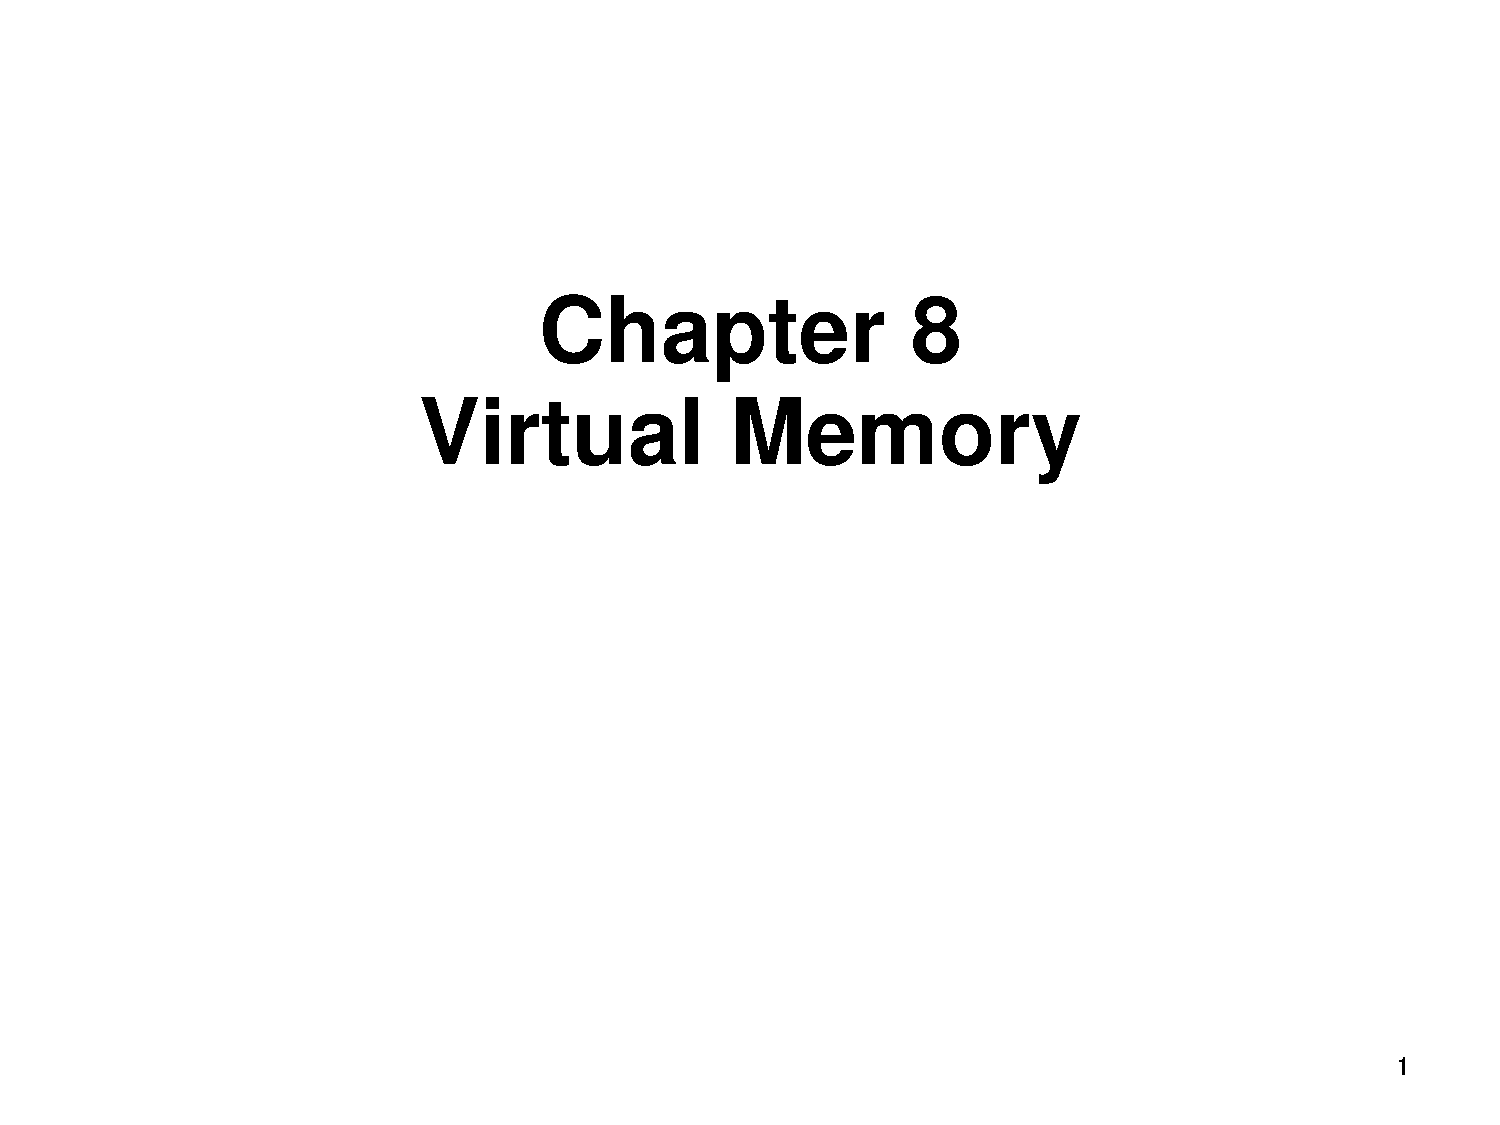
\includepdf[page=1]{08.pdf}
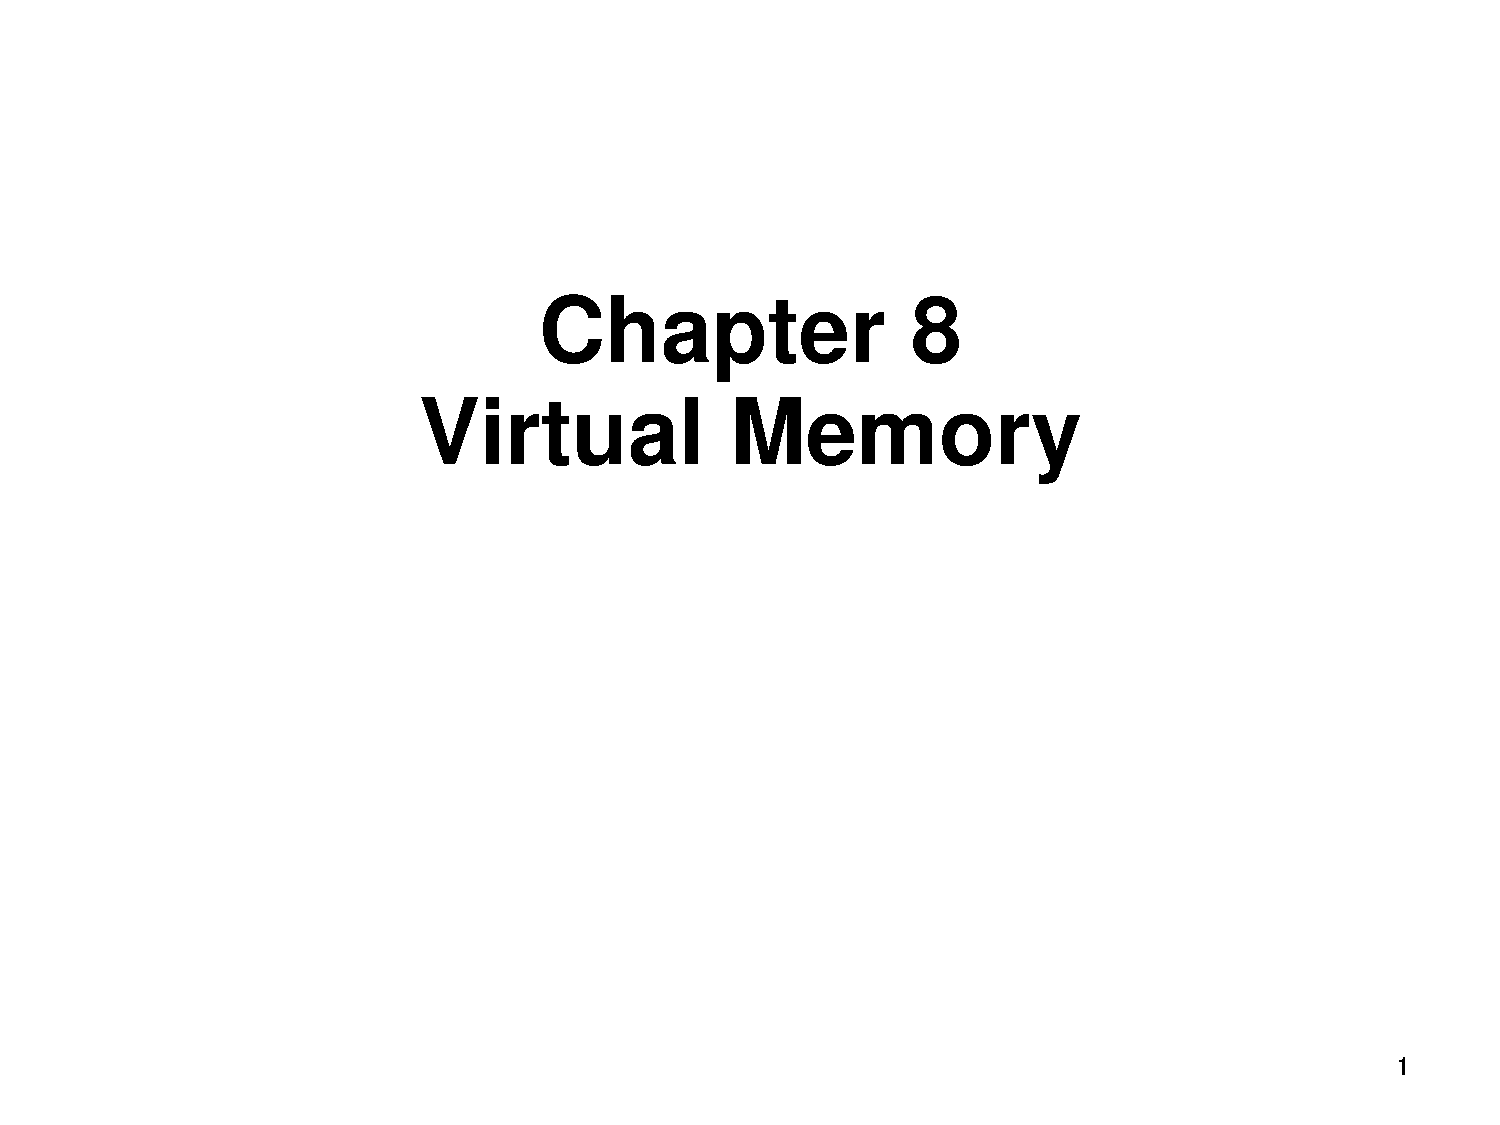
\includepdf[page=2]{08.pdf}
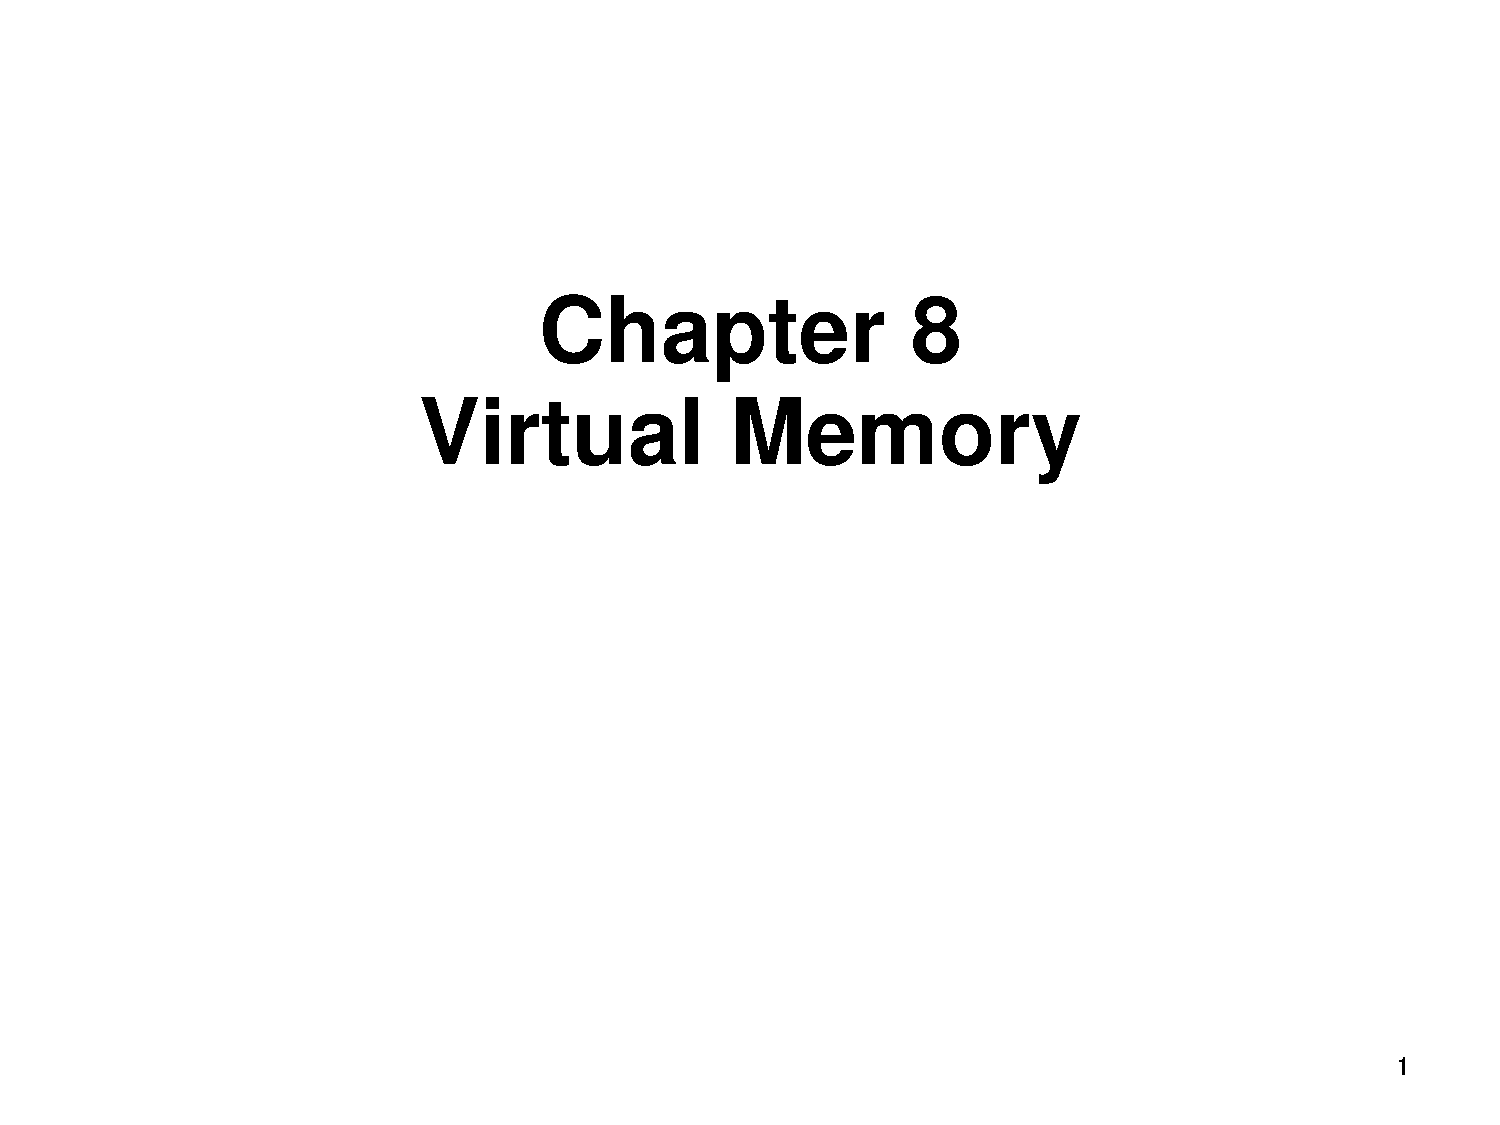
\includepdf[page=3]{08.pdf}
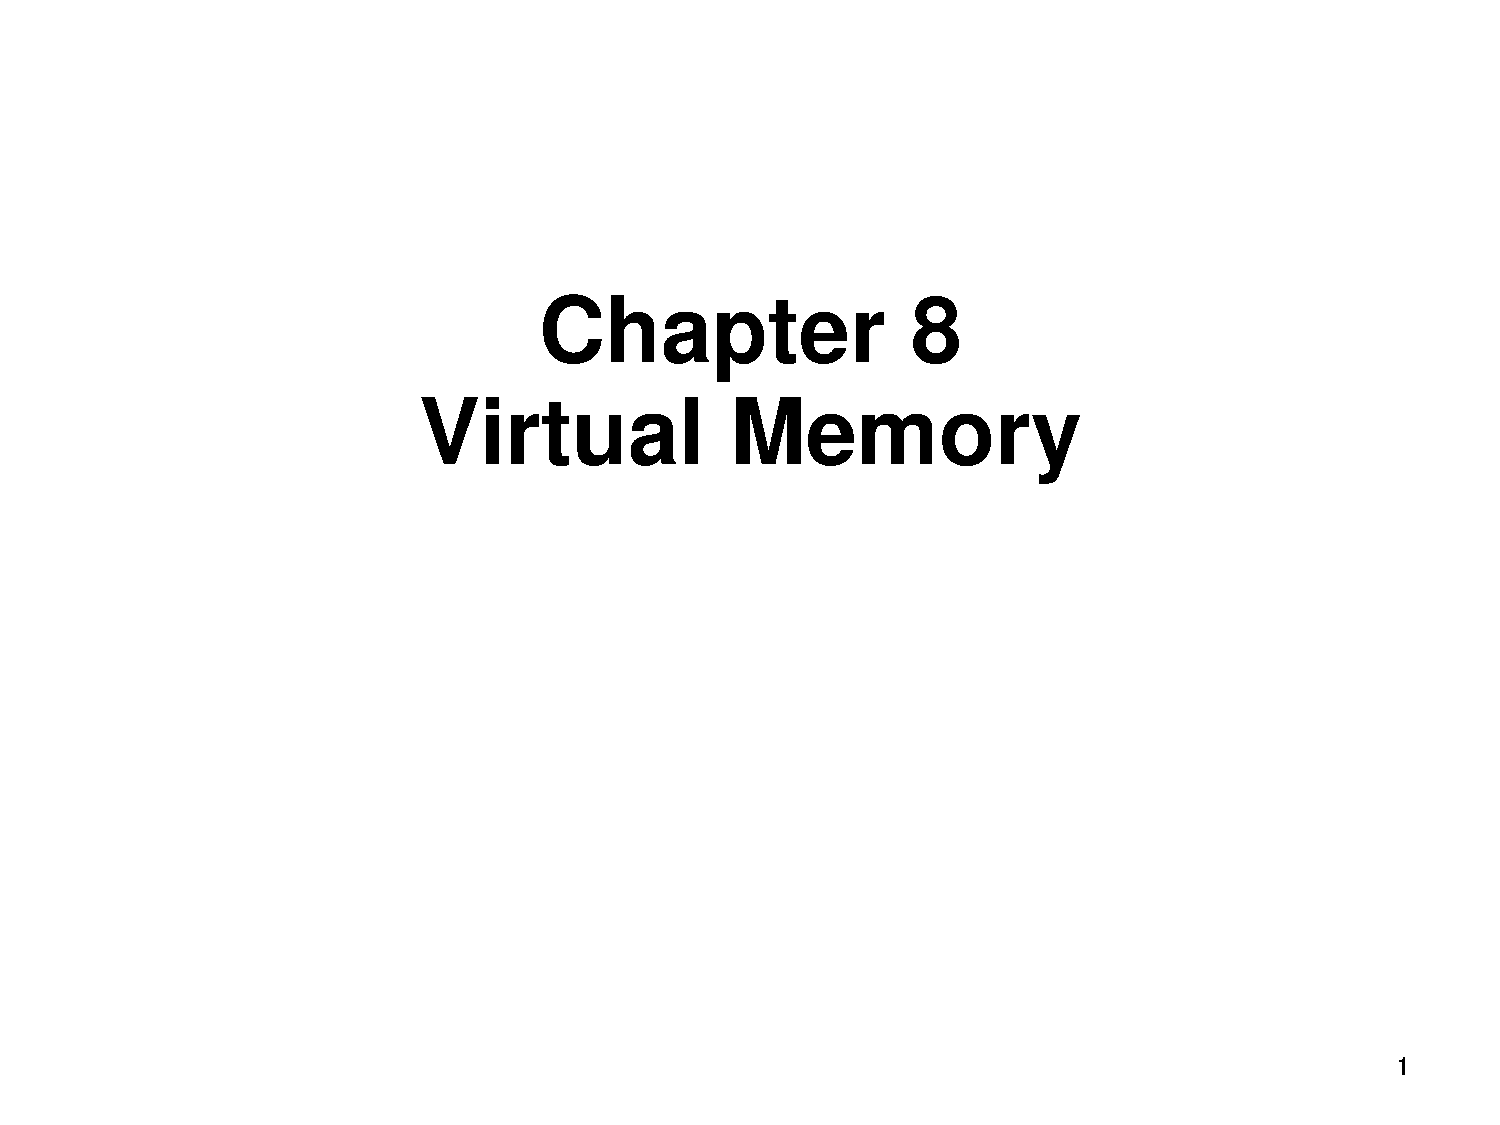
\includepdf[page=4]{08.pdf}
Now we allow the process to execute if the individual sections of the process are in memory but not necessarily consecutive. We relax the requirement that the entire process image must be in memory, only the pc and memory pointers need to be in memory for the program to run. This tricks us into thinking that there is more memory than there is.
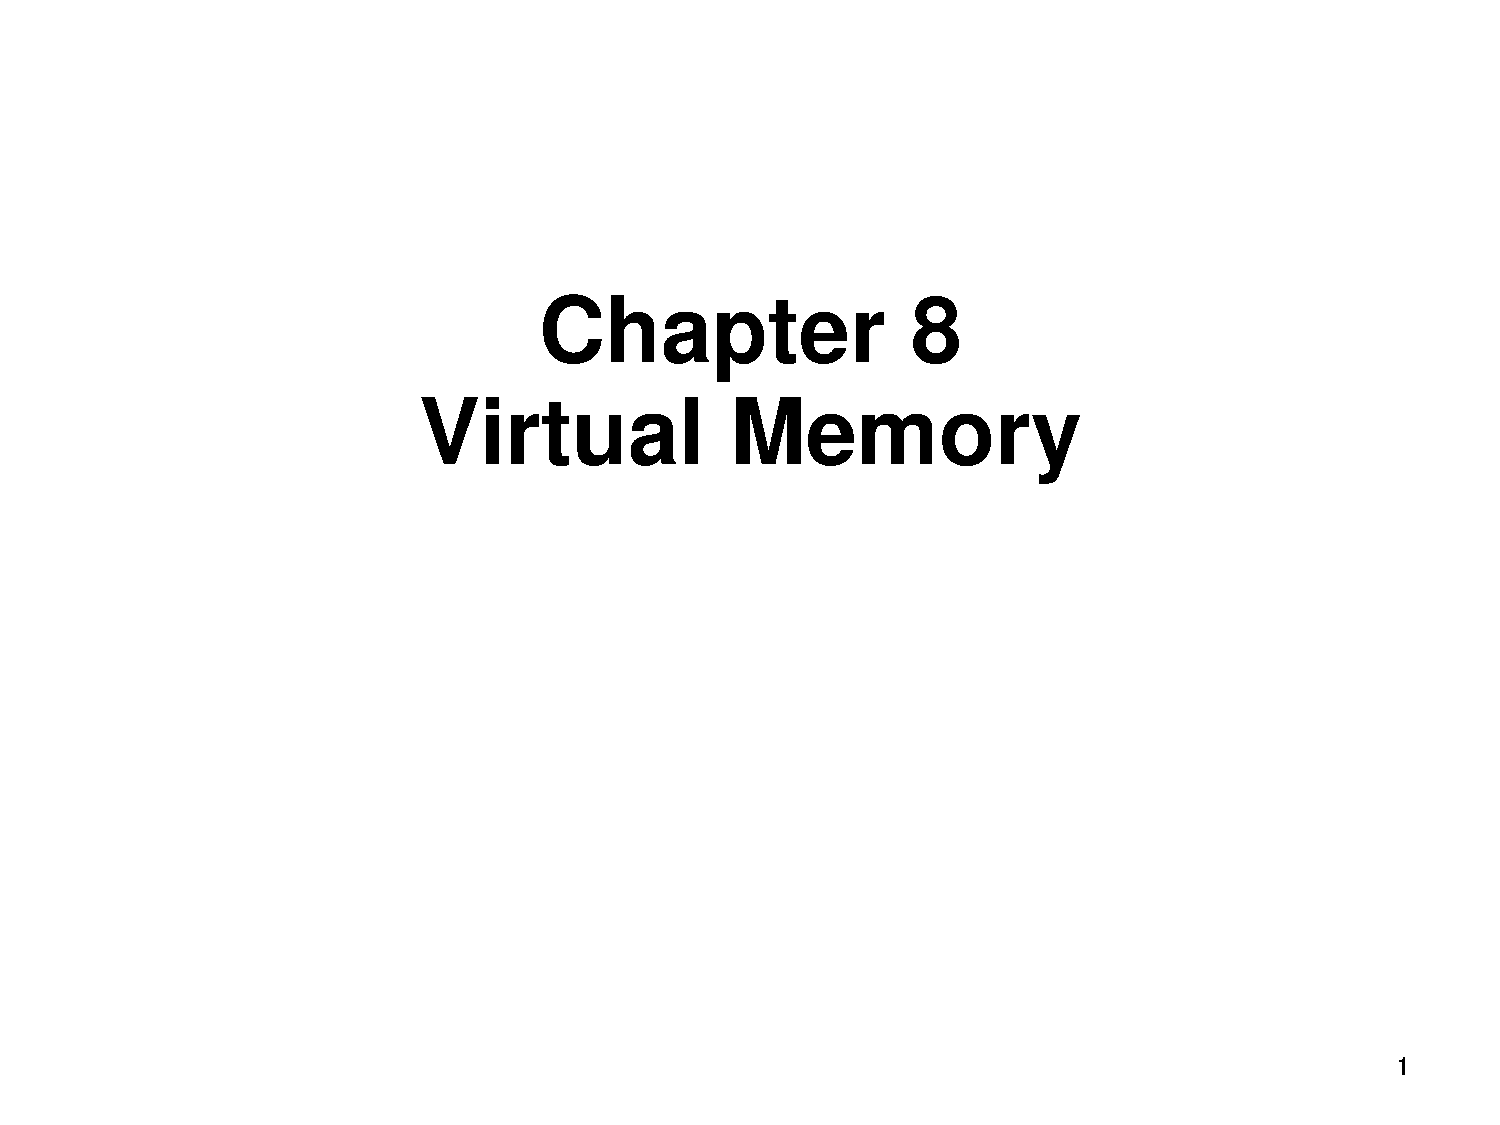
\includepdf[page=5]{08.pdf}
We need two difference addressing schemes logical addresses and real addresses. We do this with paging and segmentation (need hardware support).
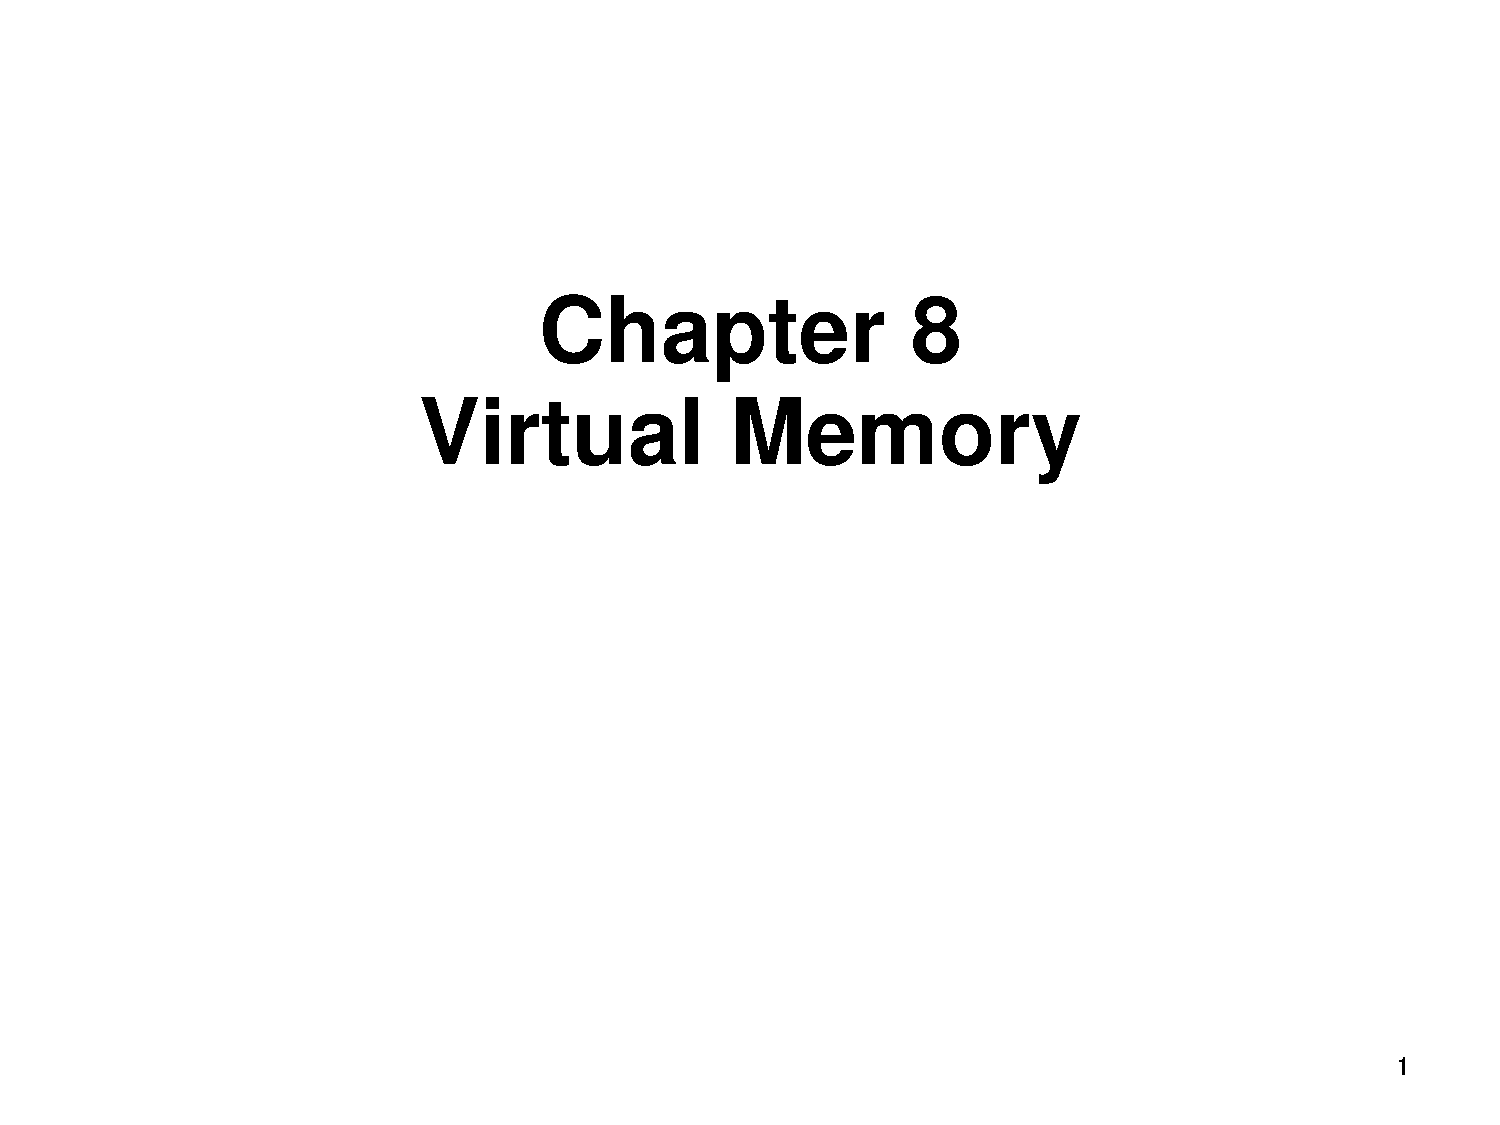
\includepdf[page=6]{08.pdf}
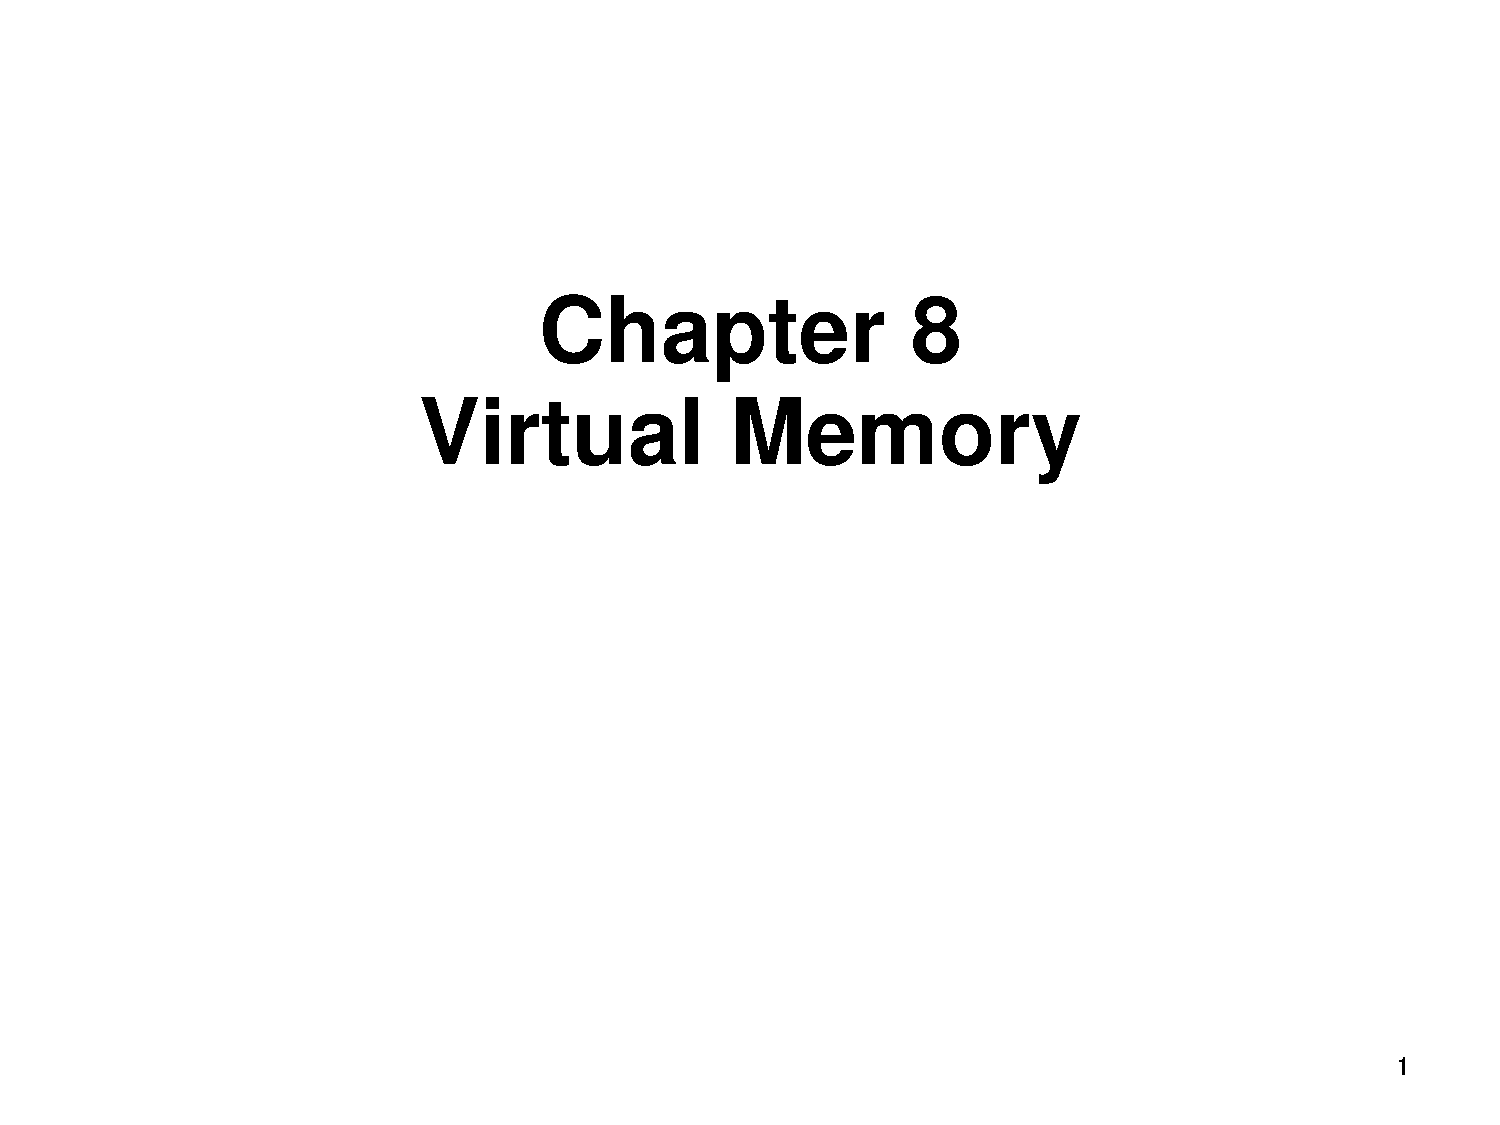
\includepdf[page=7]{08.pdf}
A process can be run withouth being a full resident in memory. We just need the next instruction to execute and the data that it needs.
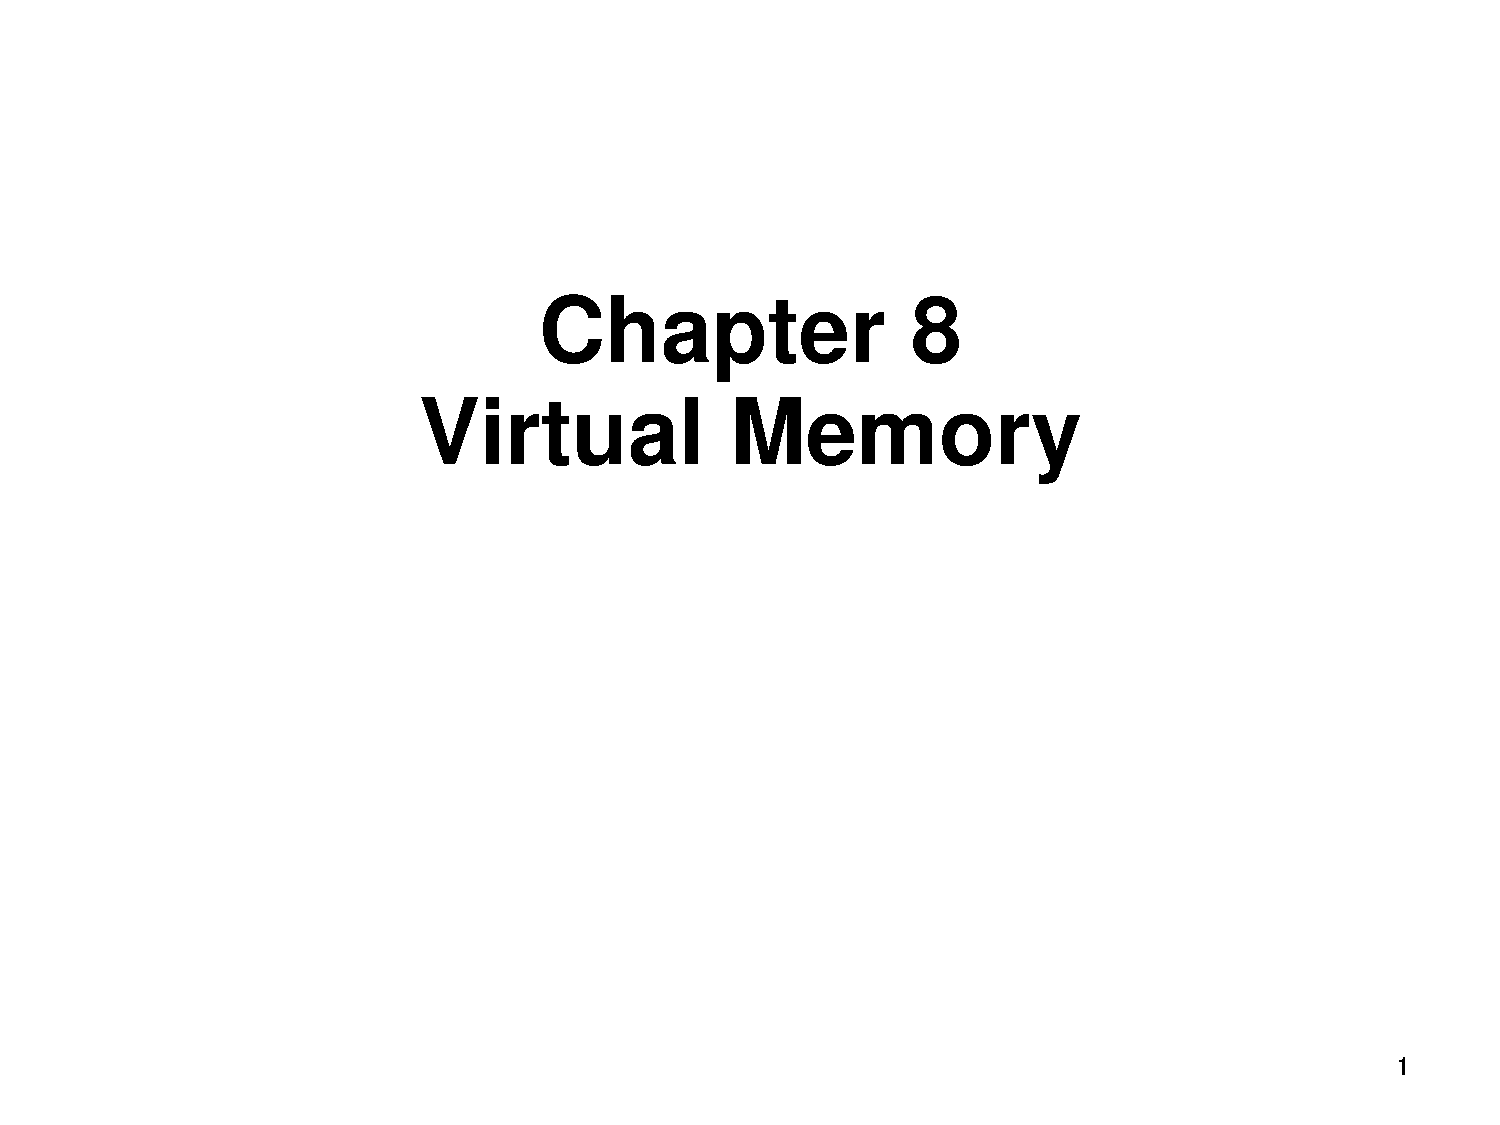
\includepdf[page=8]{08.pdf}
We keep executing until we need something that is not in main memory, where we trigger a interrupt (page fault) that blocks the process and retrieve what we need. We have to check the memory address table to see if the necessary data is in memory (has a table).
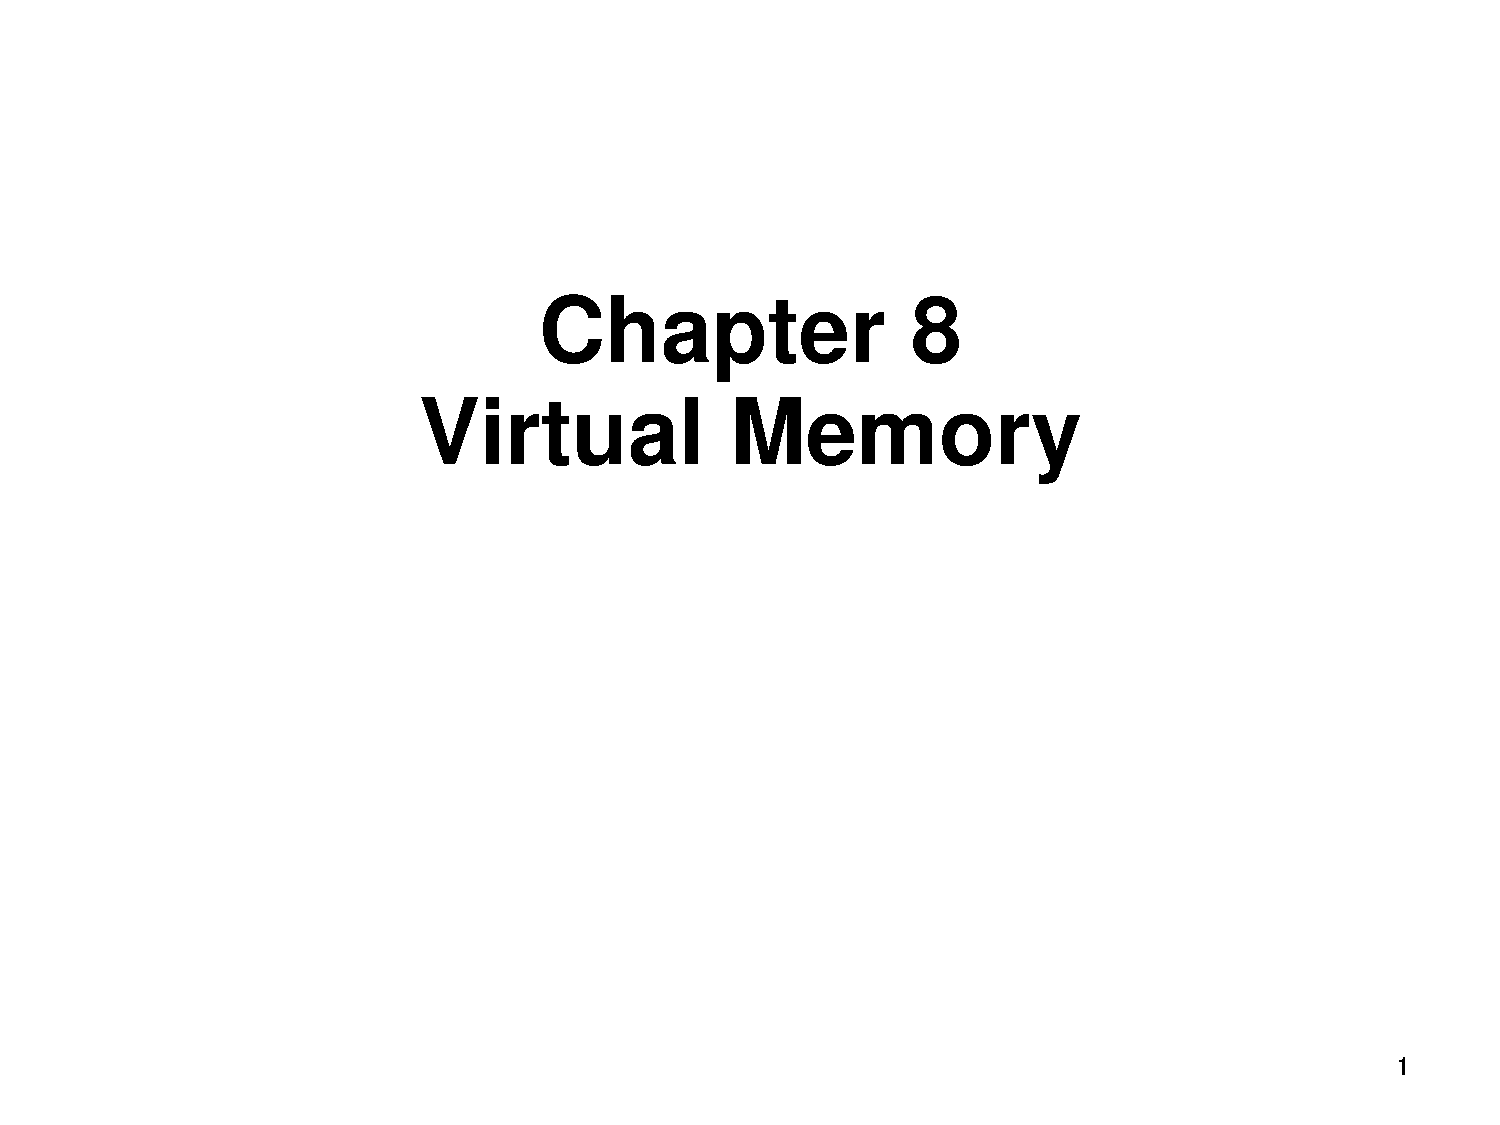
\includepdf[page=9]{08.pdf}
We decide what portion of process is in main memory, it becomes important when we do paging.
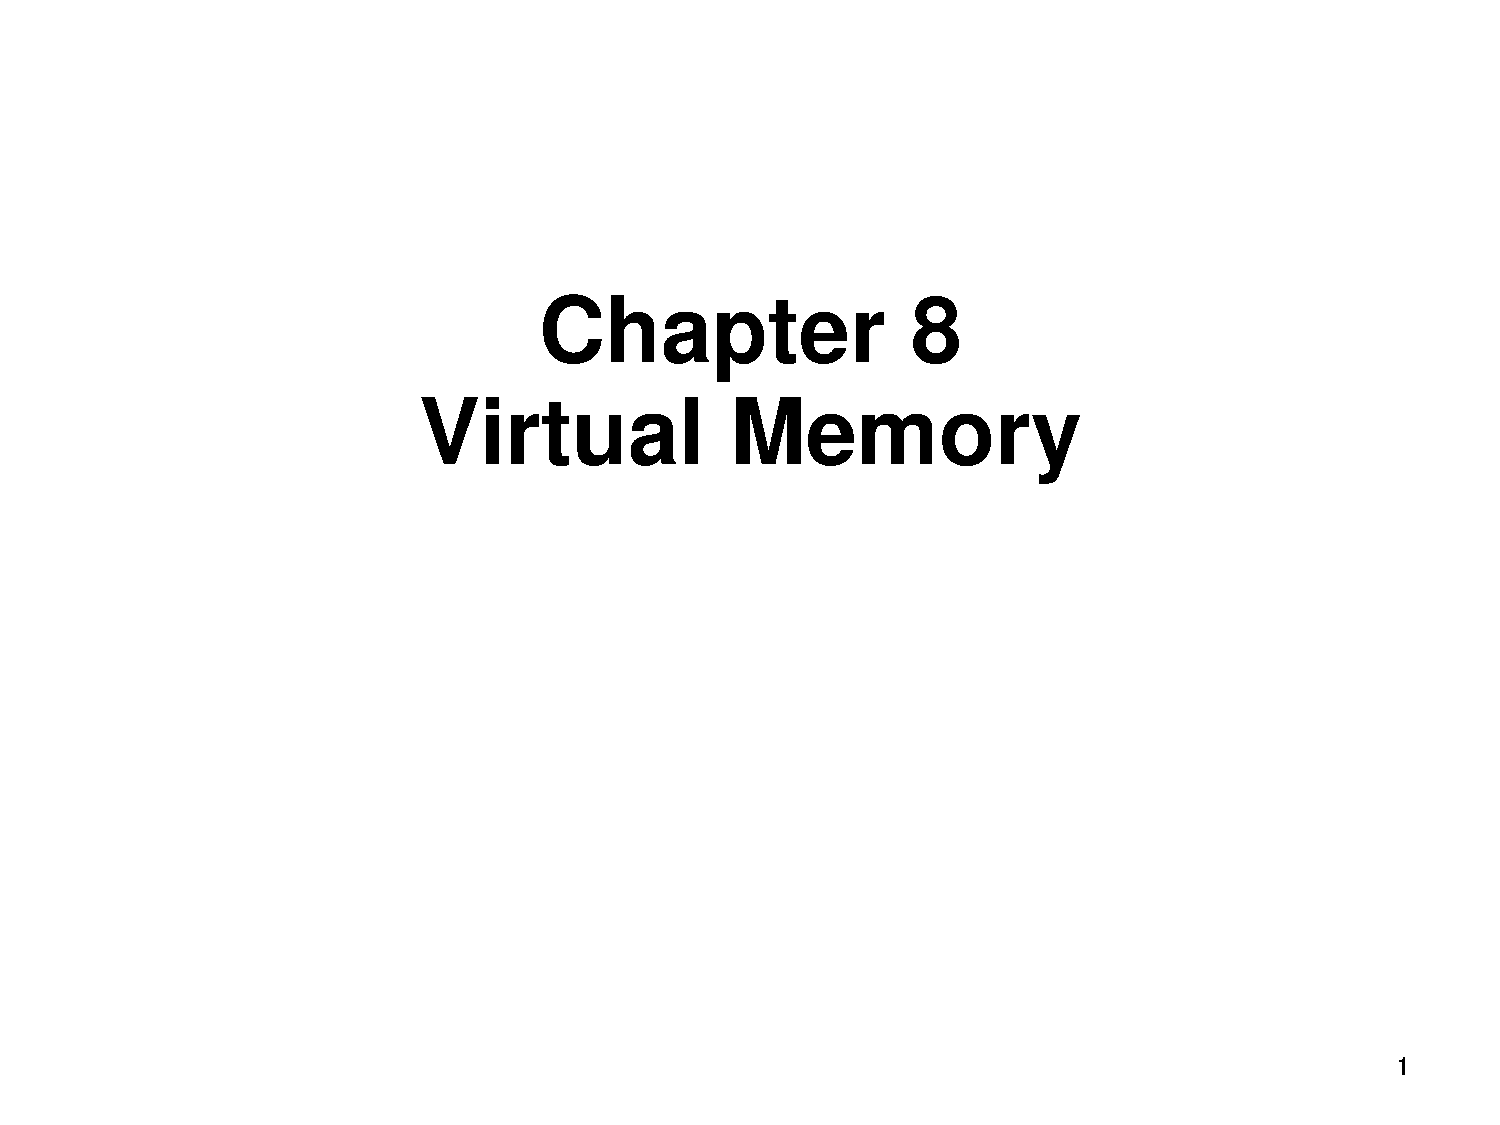
\includepdf[page=10]{08.pdf}
The operating system knows to load data if it cannot find it in the page table (page fault). The service routine for a page fault finds what data is needed and laods it into memory.
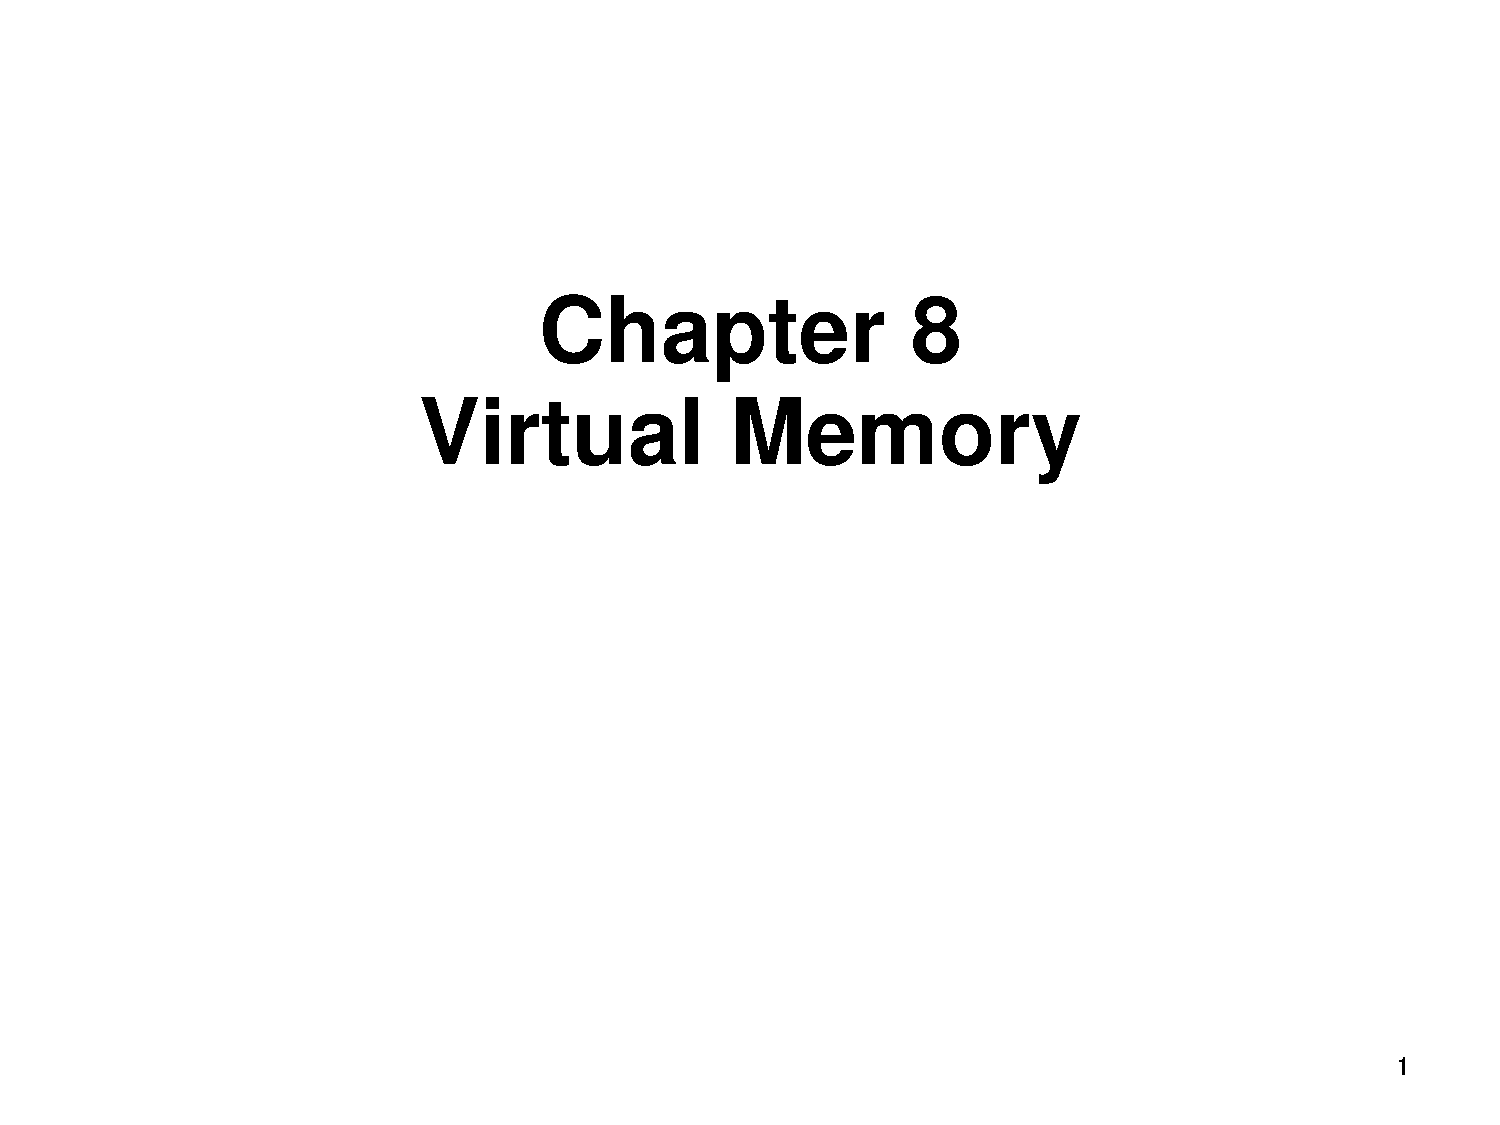
\includepdf[page=11]{08.pdf}
This lazy loading scheme tends to actually be more efficient. We want to load multiple frames into memory because we tend to need code that is in the same area of secondary storage and reading is costly.
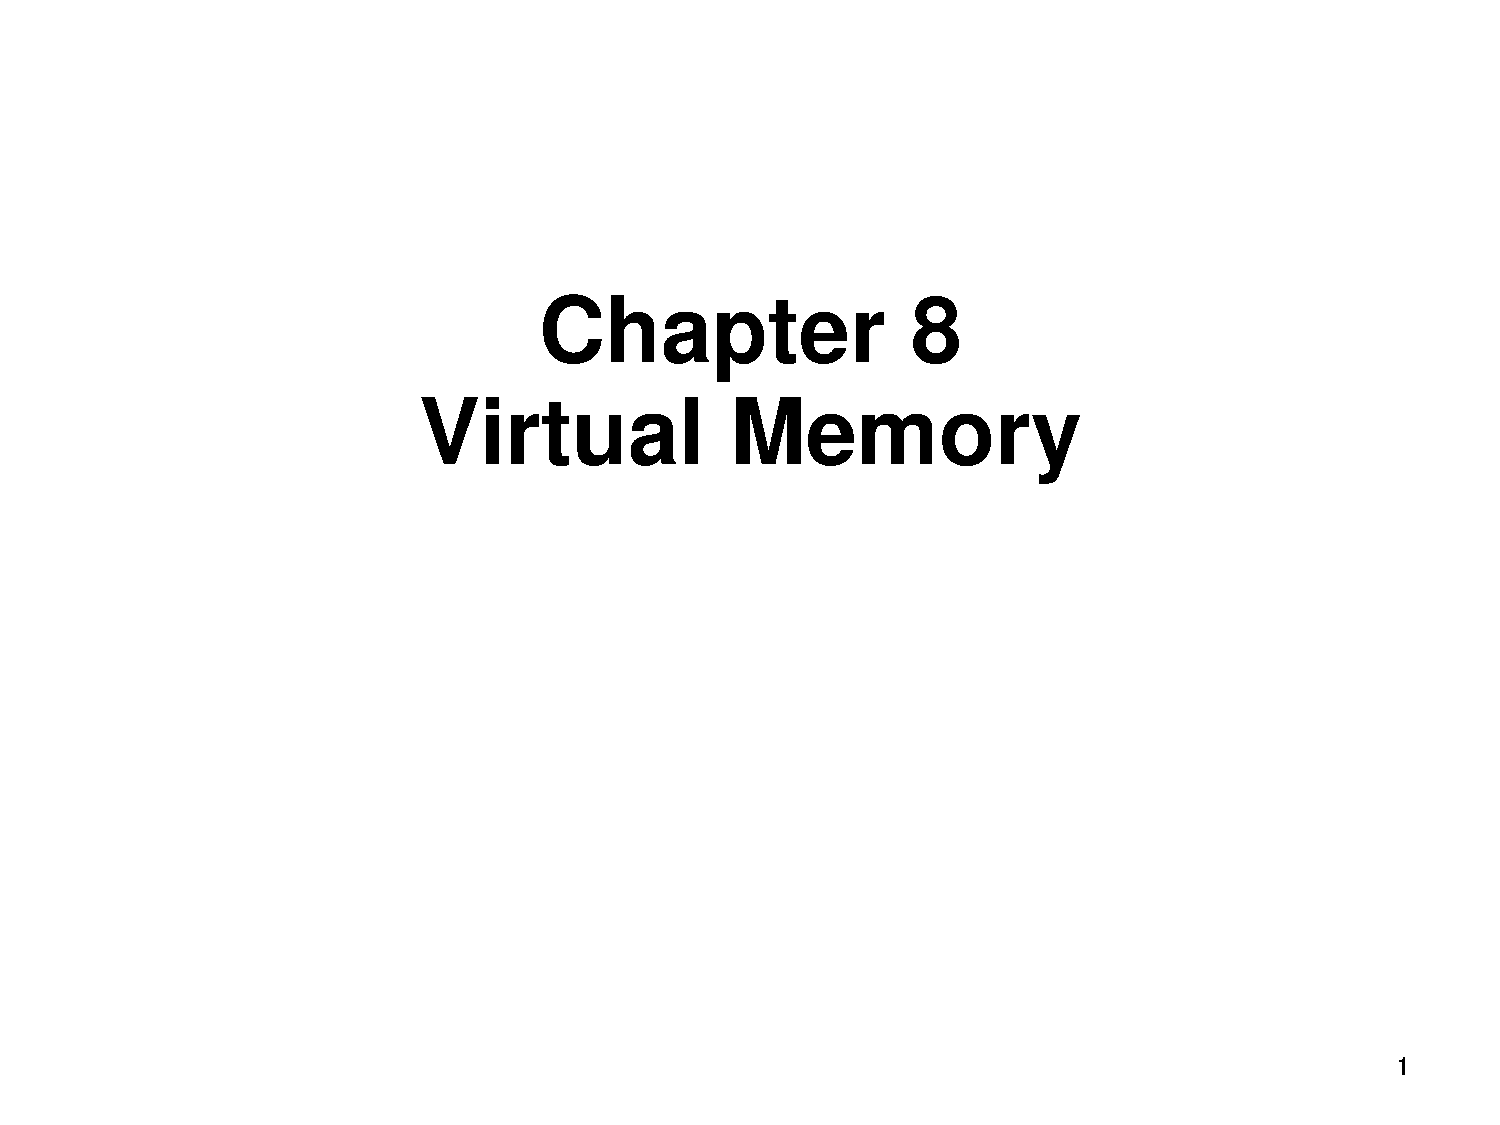
\includepdf[page=12]{08.pdf}
We can exceed the physical memory size.
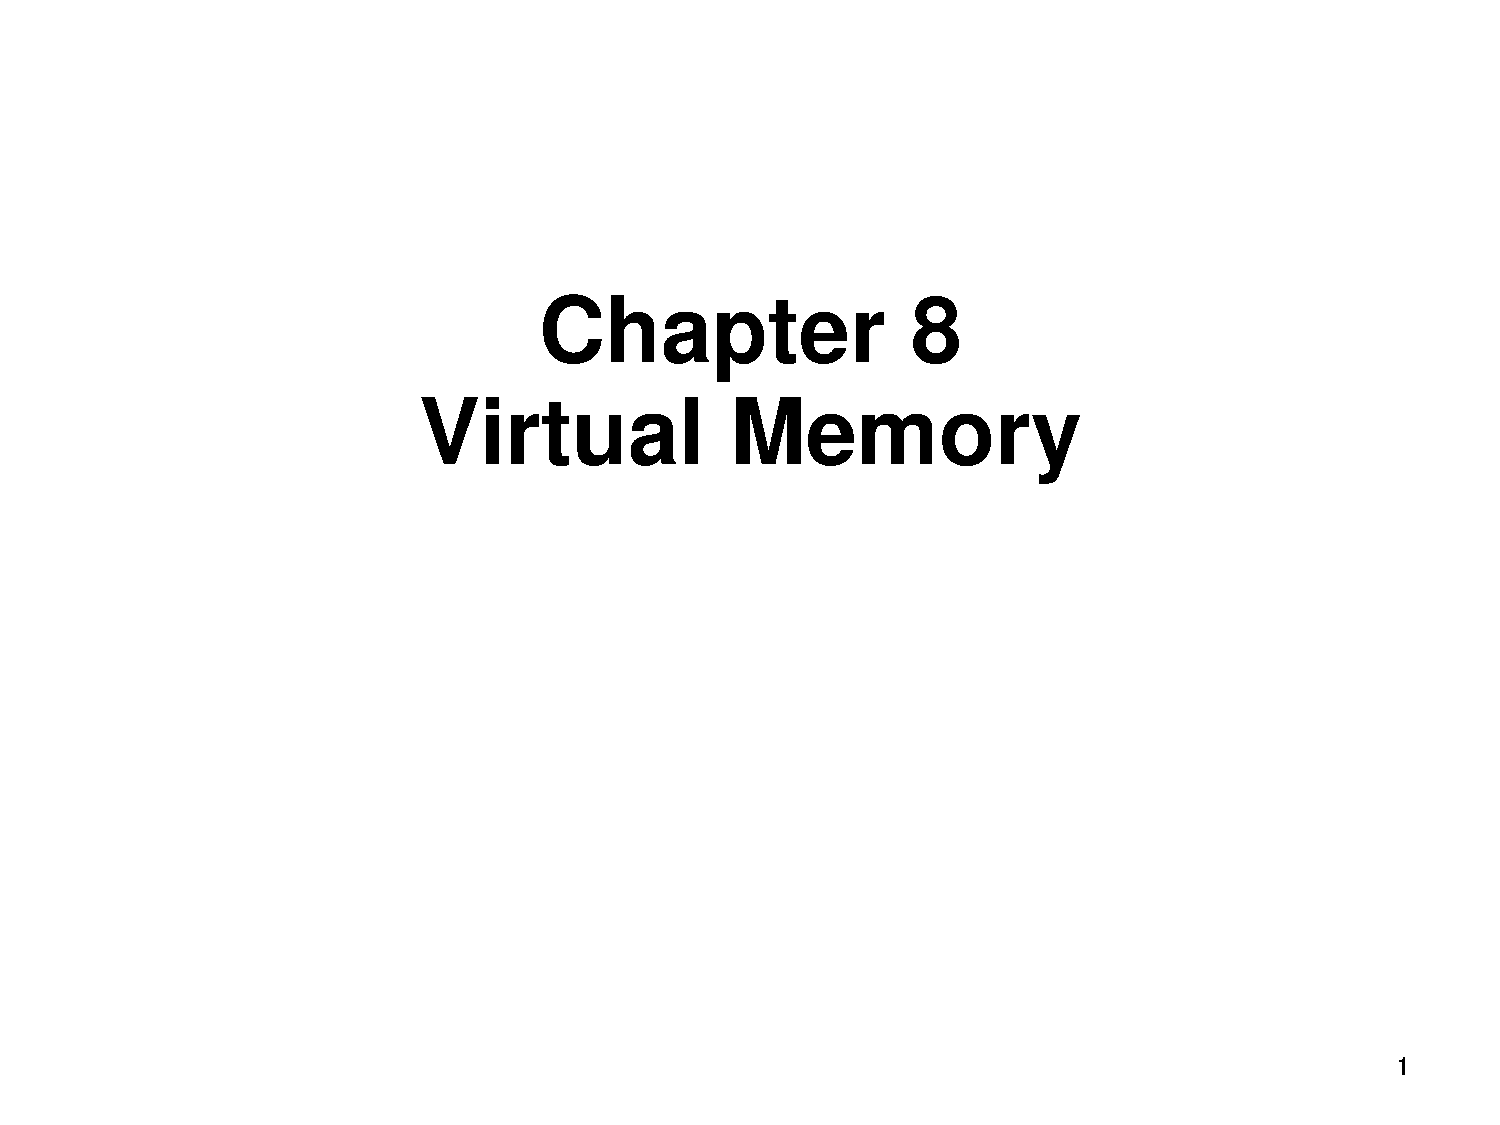
\includepdf[page=13]{08.pdf}
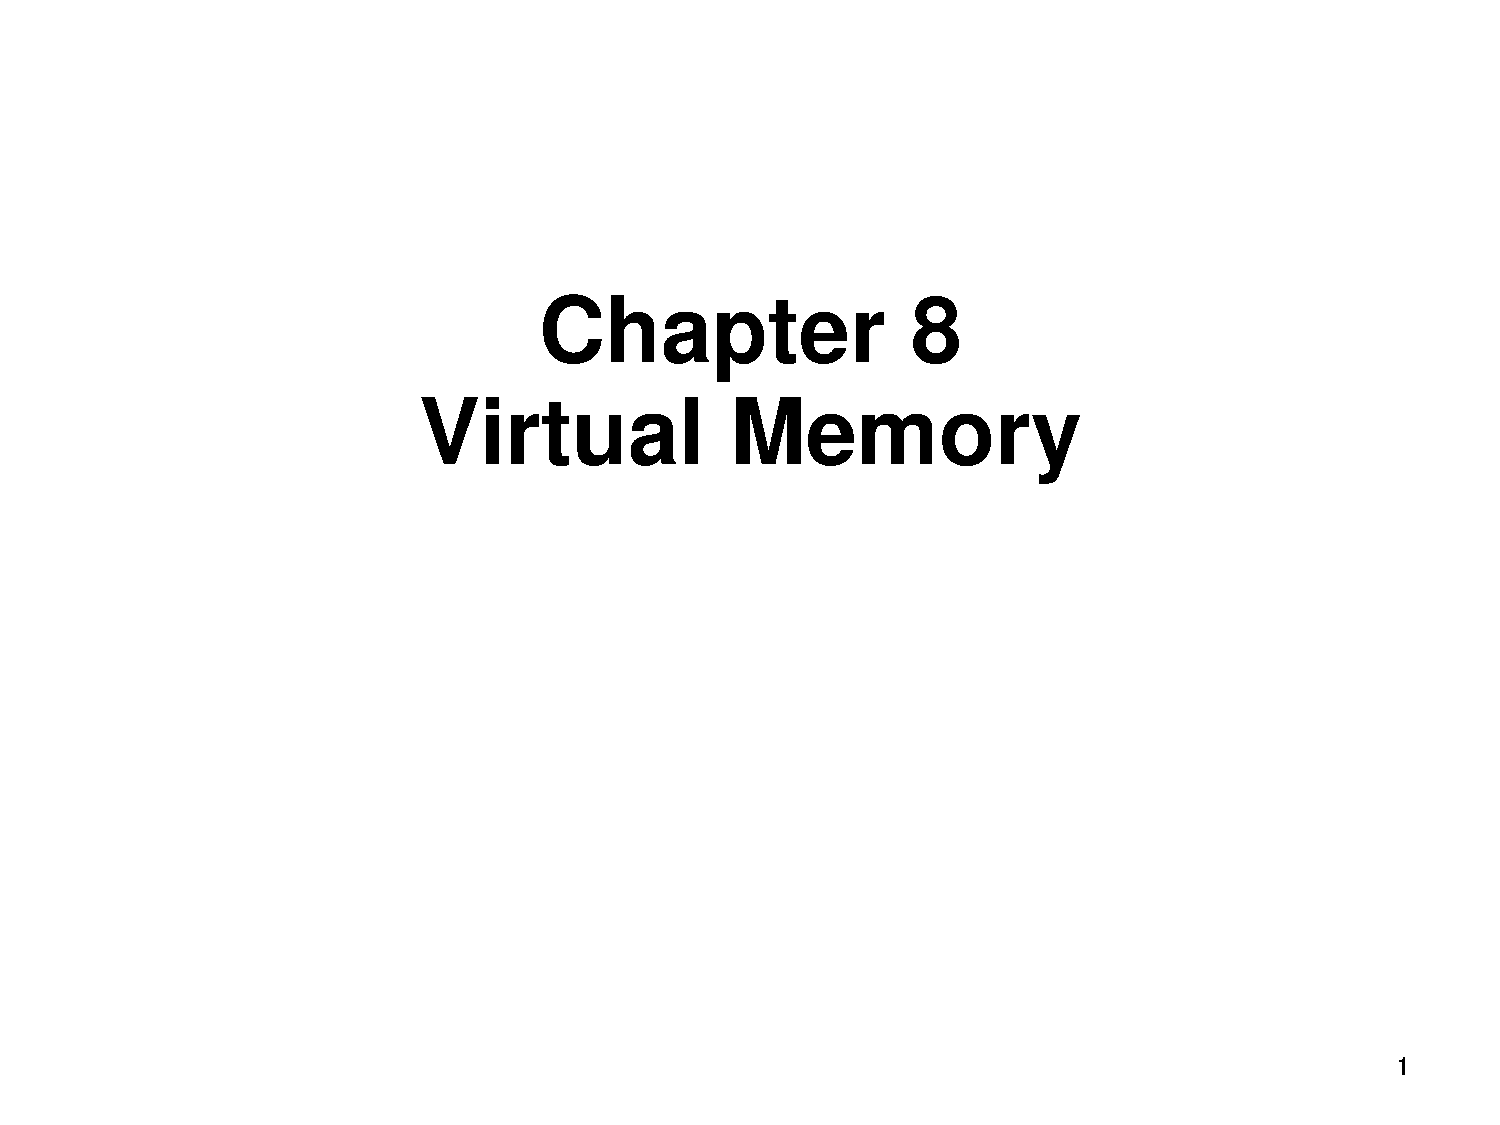
\includepdf[page=14]{08.pdf}
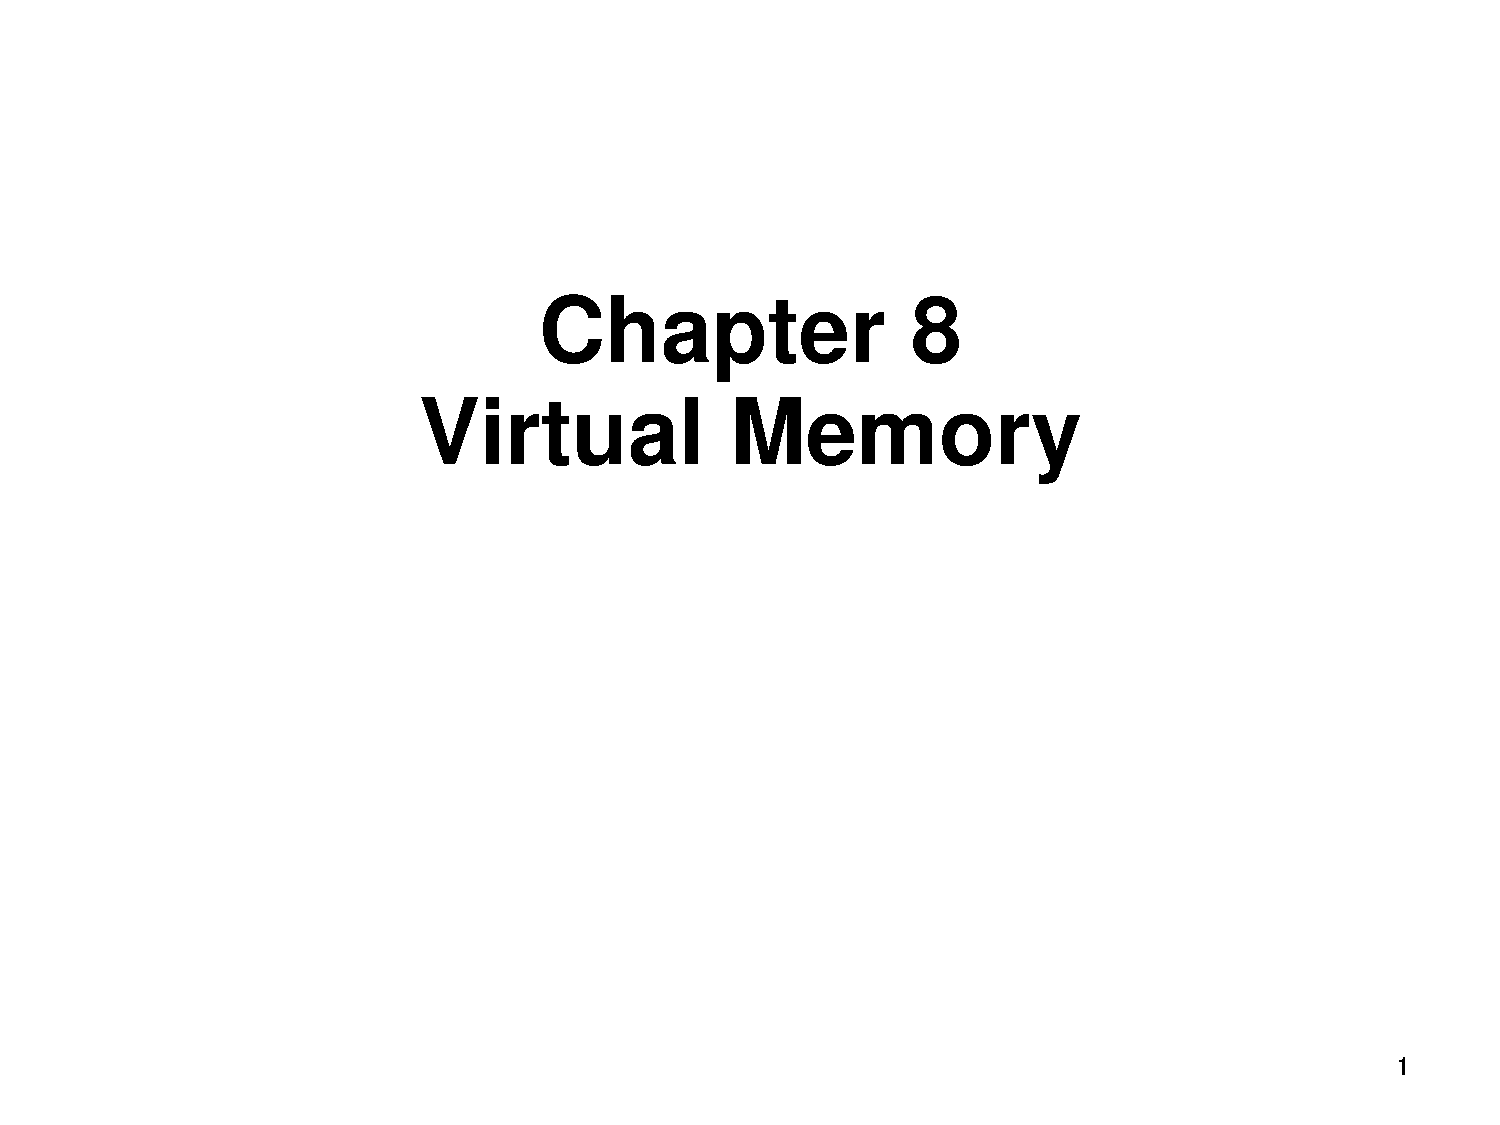
\includepdf[page=15]{08.pdf}
What happens when we run out of memory? Thrashing is when we reach max copacity having to swap something out to put something in so we hit waaaaay more page faults and slows everything down. There are some very clever algorithms that decide what we should take out in order to load the memory that we need at the moment.
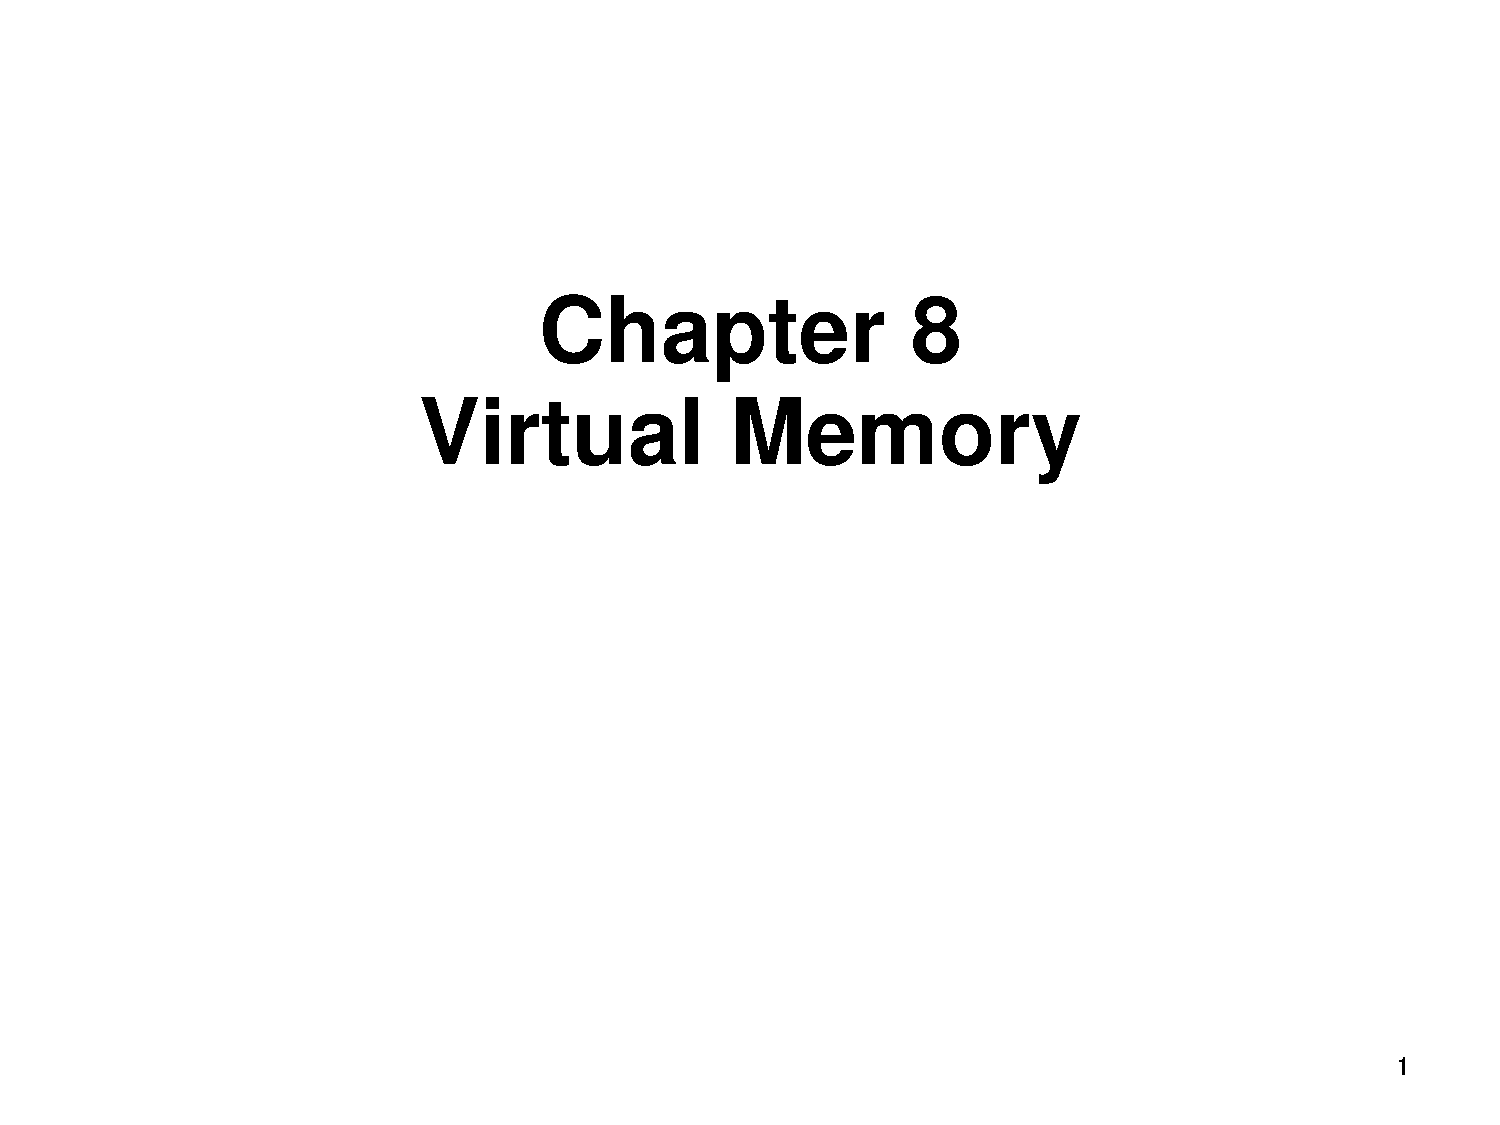
\includepdf[page=16]{08.pdf}
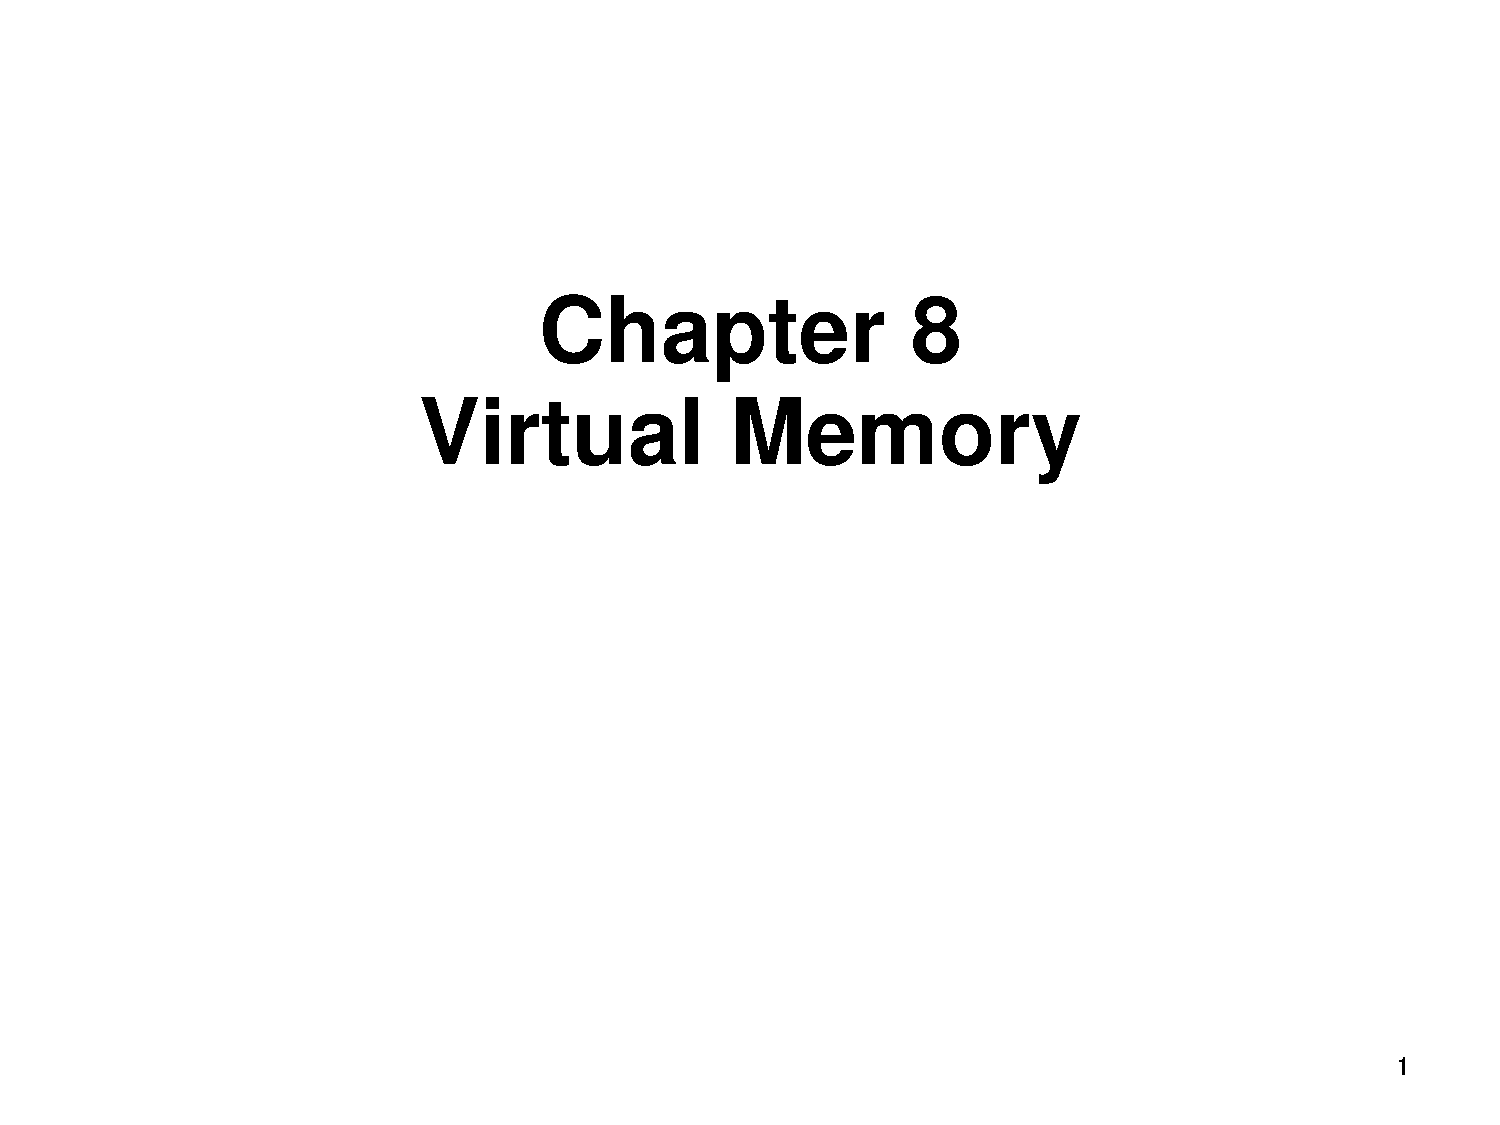
\includepdf[page=17]{08.pdf}
Most algorithms used to chose what memory to remove, are based on the principle of locality.
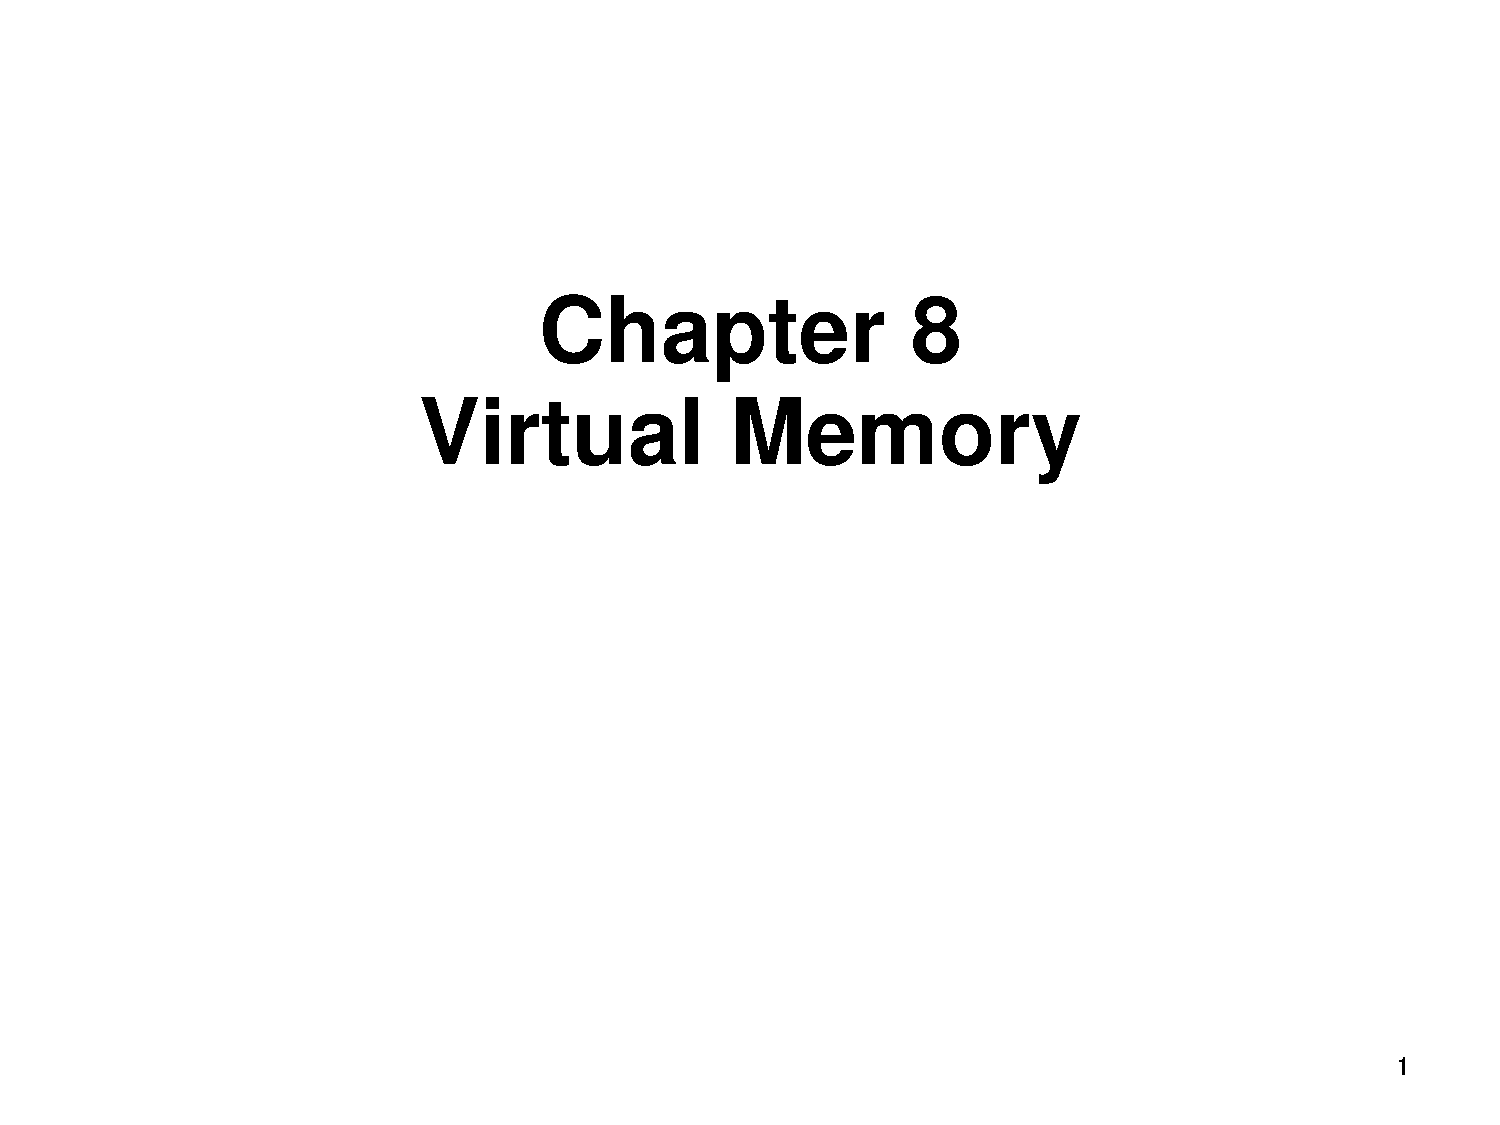
\includepdf[page=18]{08.pdf}
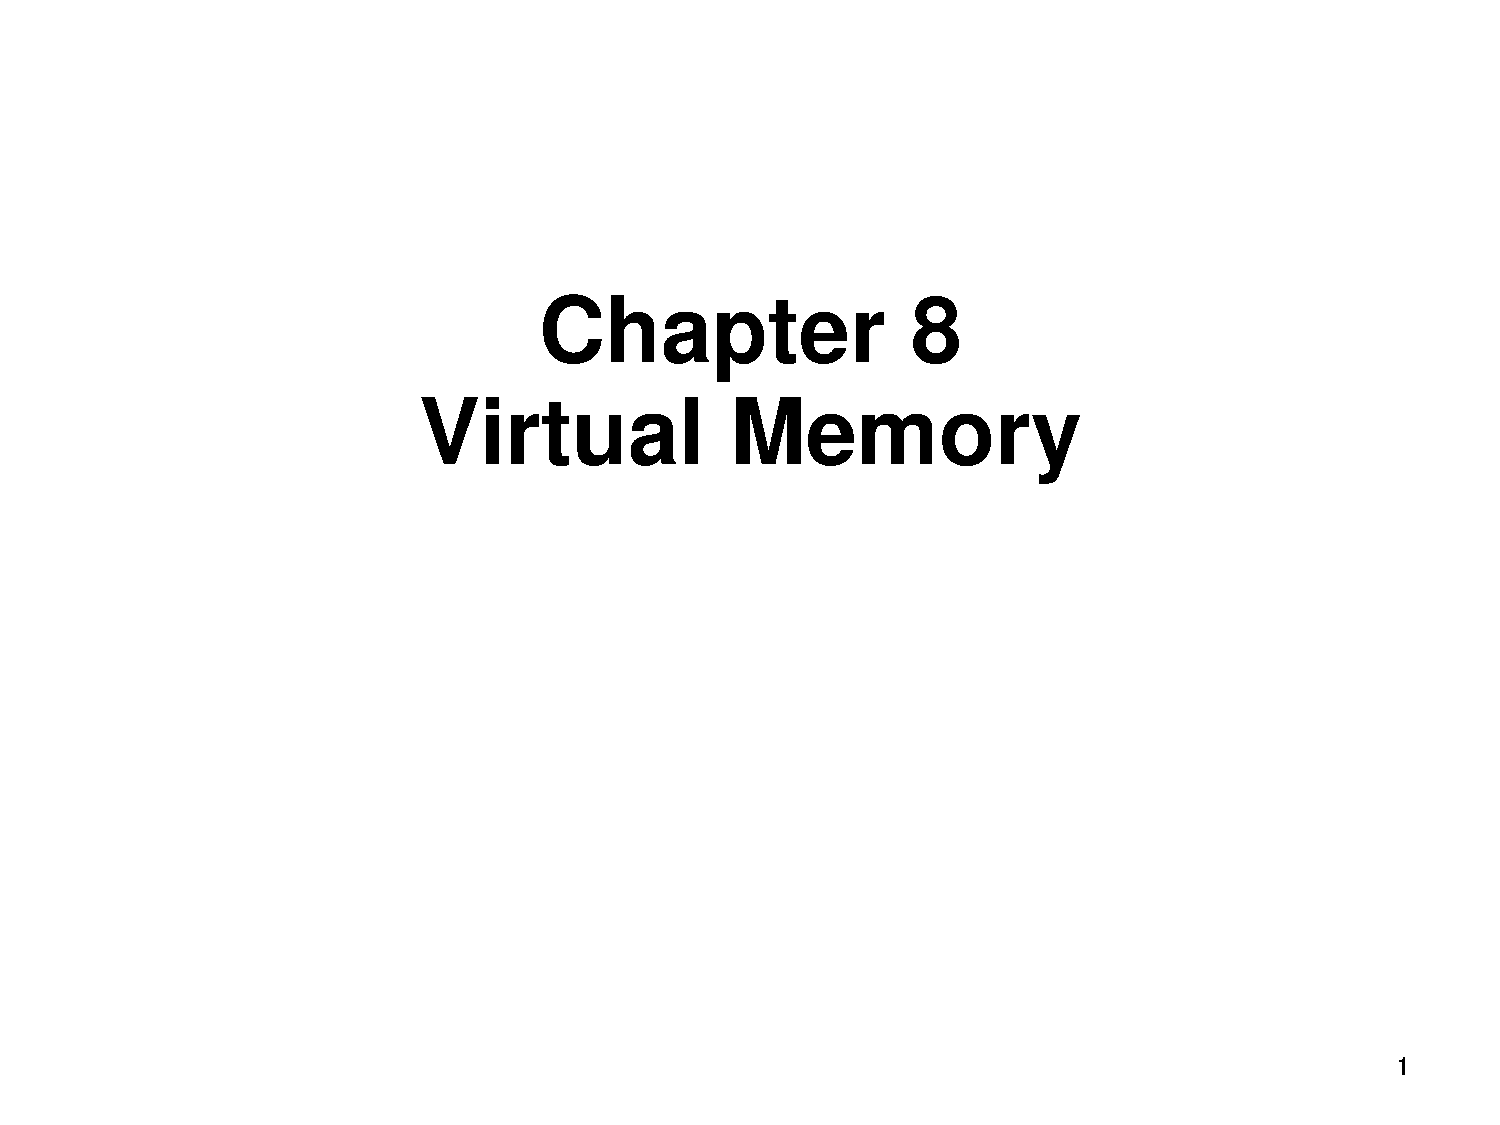
\includepdf[page=19]{08.pdf}
In the page table we map the virtual address to a real address. Page table entries we have protection bits, a bit indicating if the page has been modified and needs to be written back to disk, control bits, and the frame number in main memory.
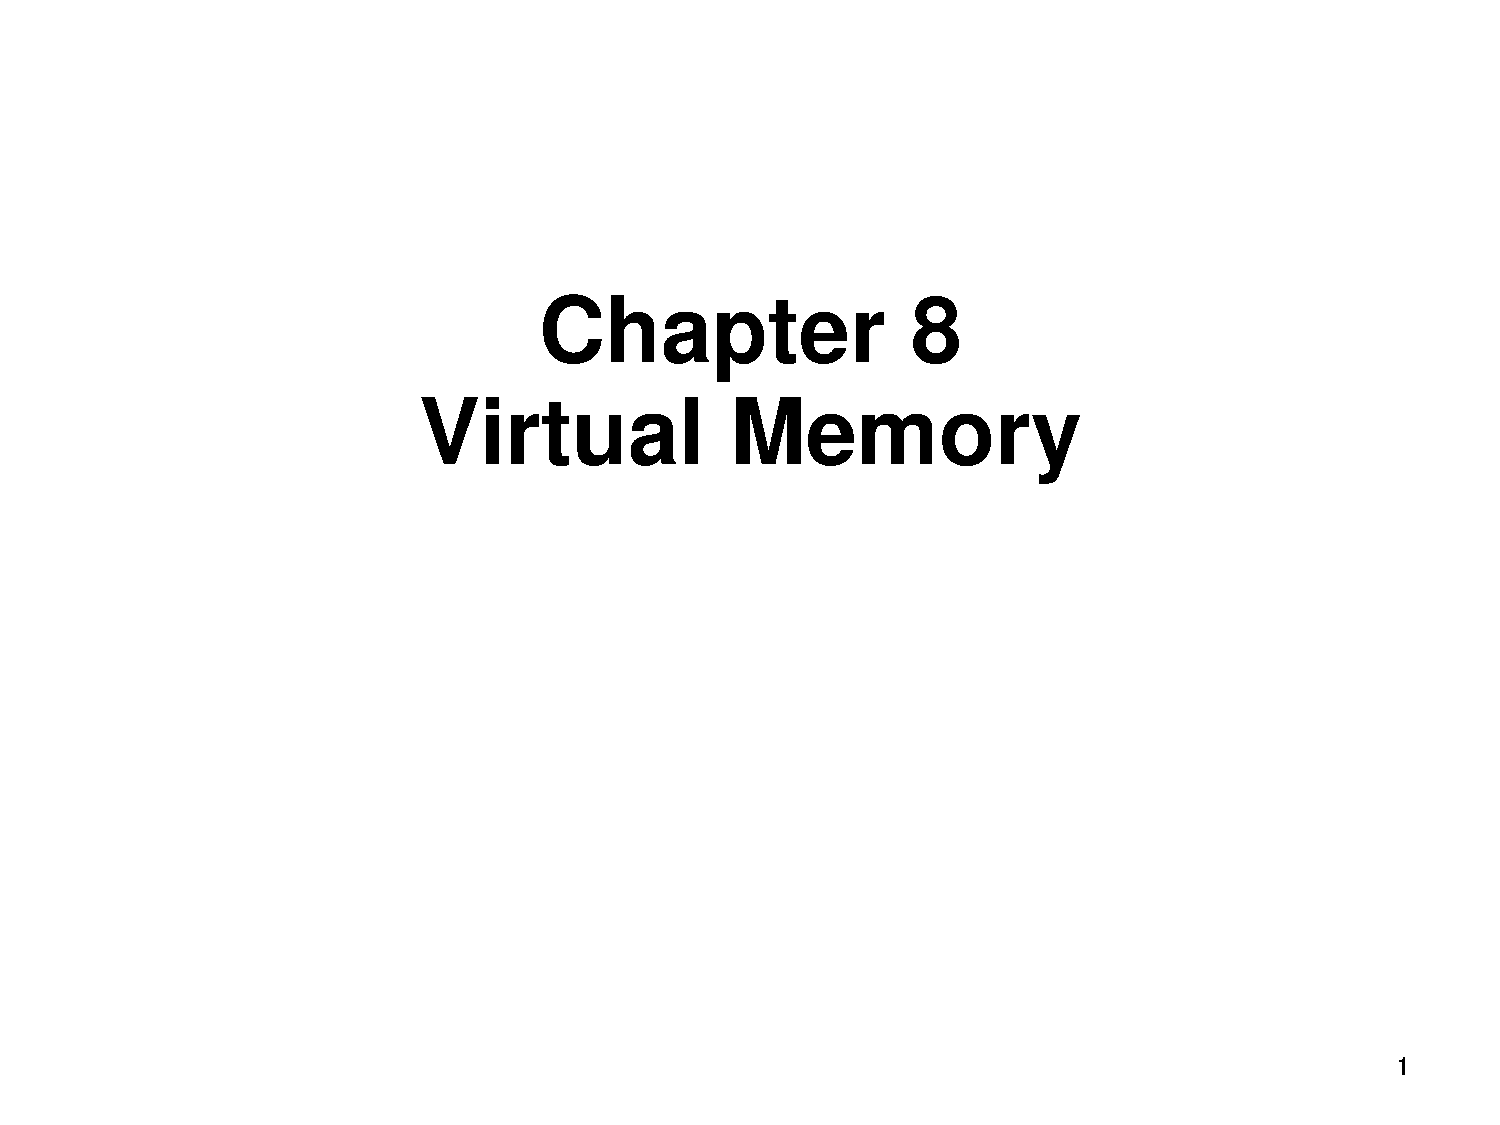
\includepdf[page=20]{08.pdf}
Start with page number, add to page table pointer to get page table entry. If that entry exists it maps to the frame number. Copy the offset over and add it to the end of the frame number and this is the real address.
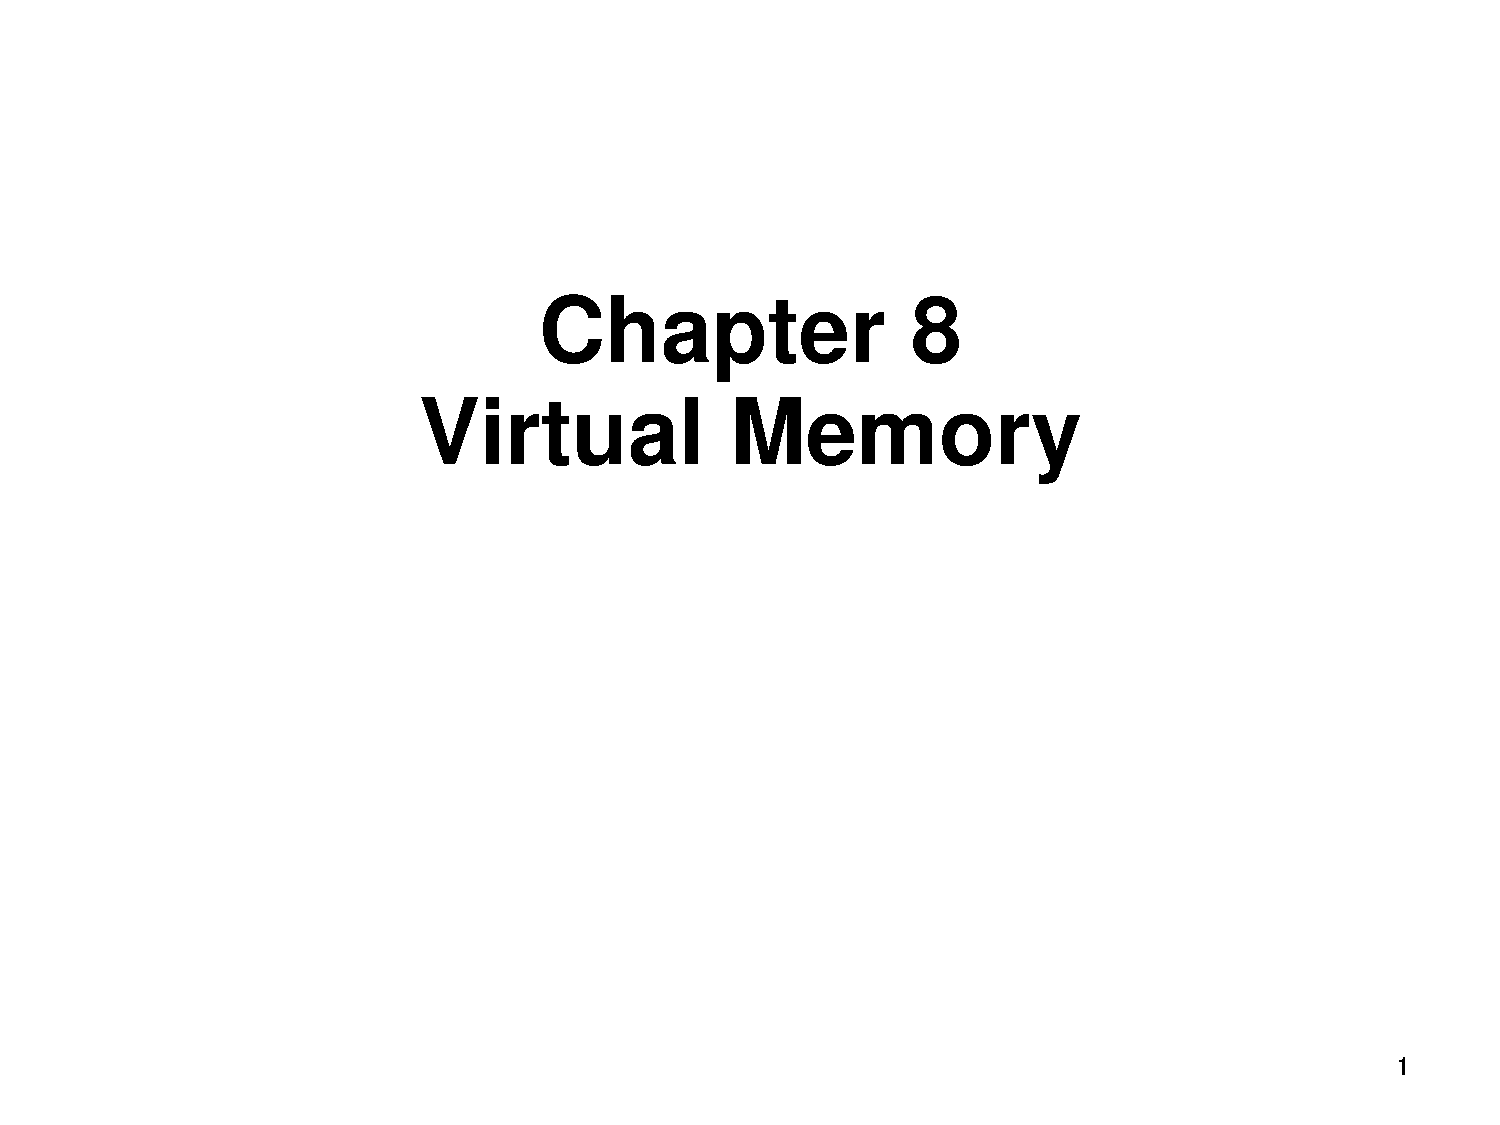
\includepdf[page=21]{08.pdf}
Page tables are fucking huuuuuuge
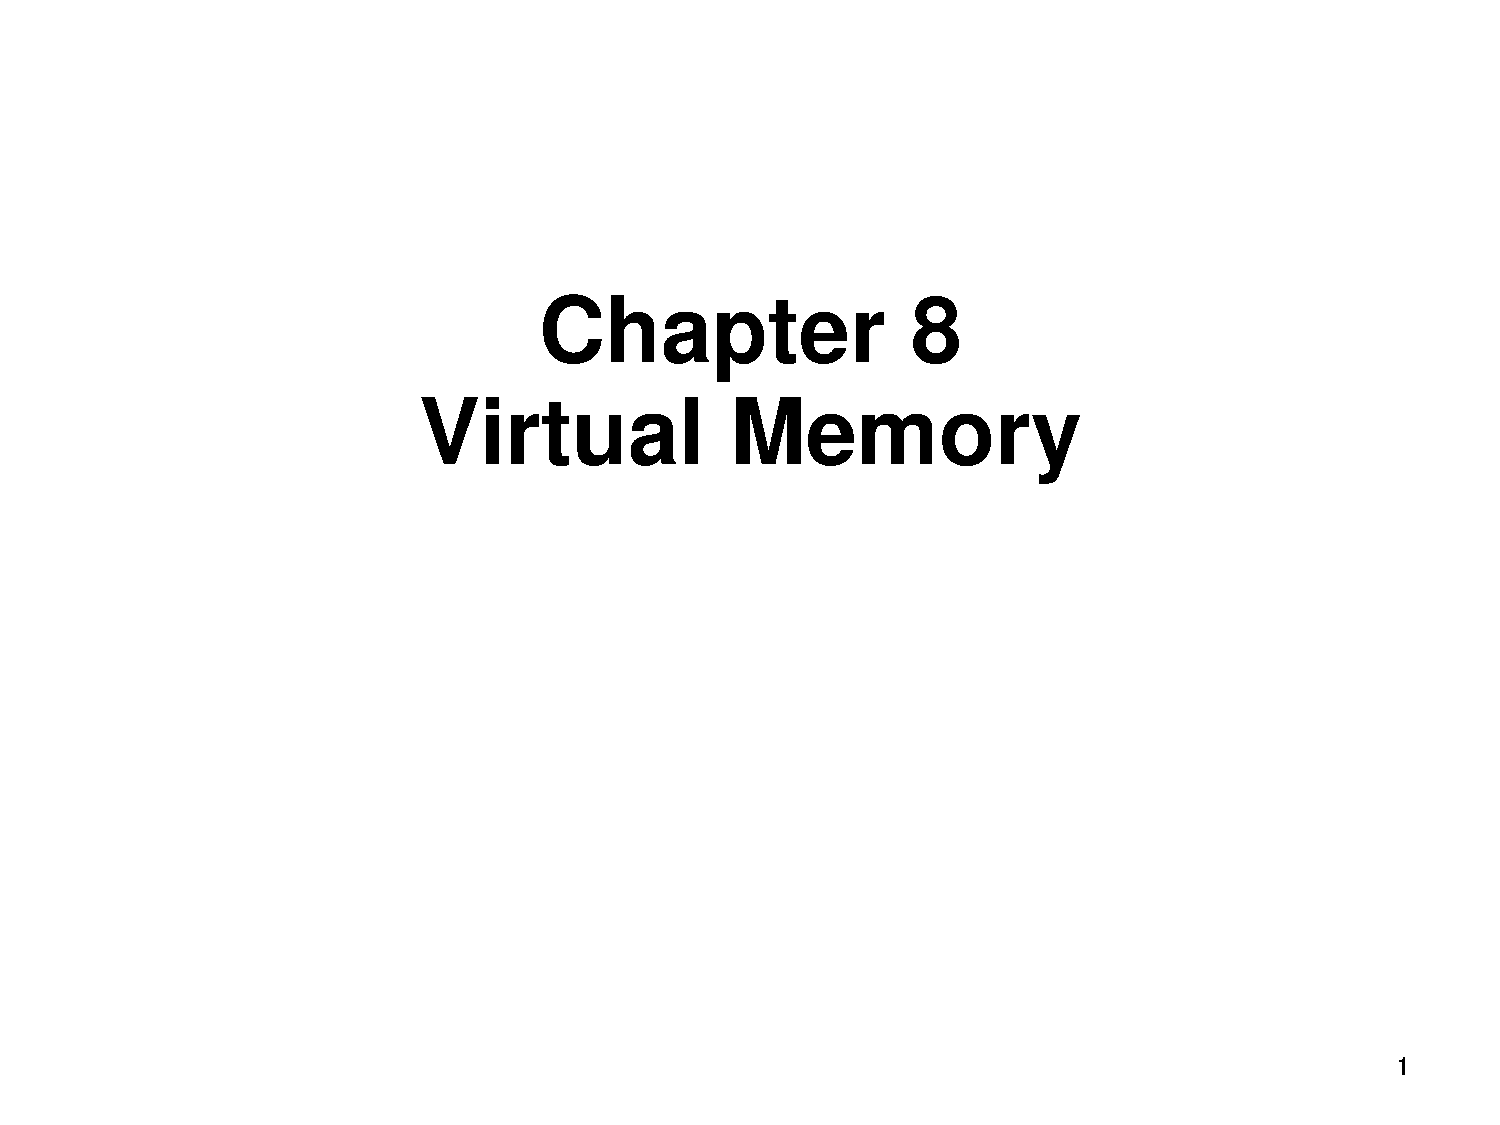
\includepdf[page=22]{08.pdf}
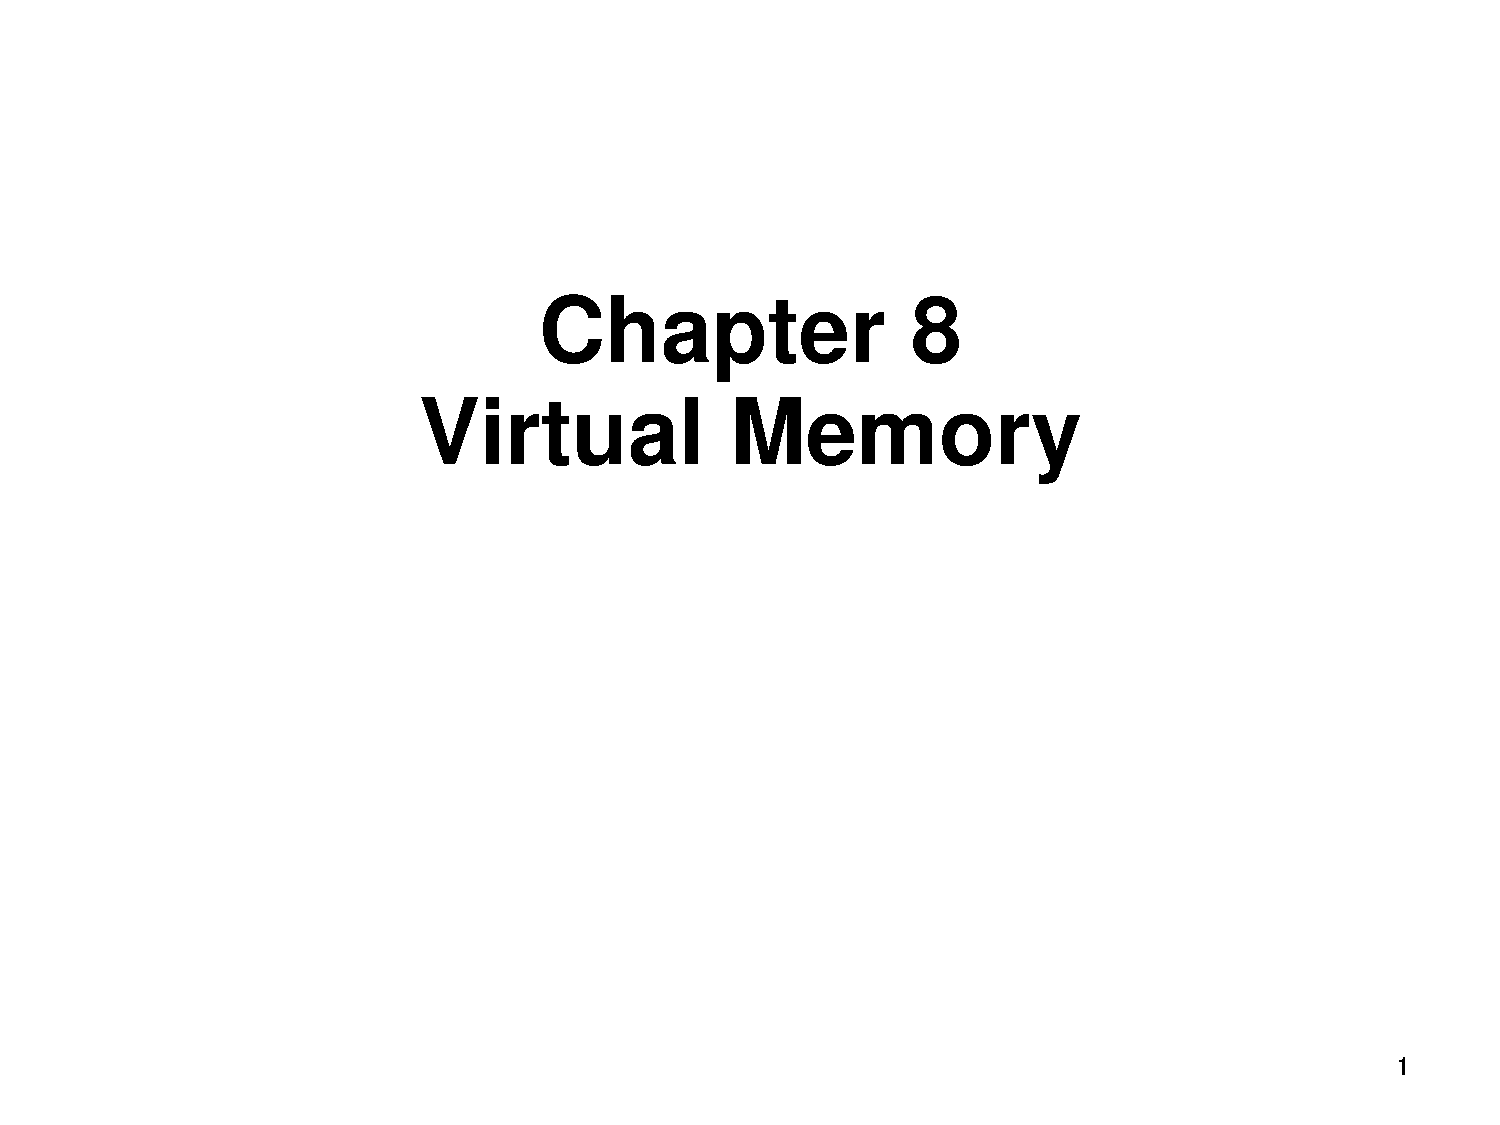
\includepdf[page=23]{08.pdf}
Now we use two levels of page tables. Basically tables that map to page tables.
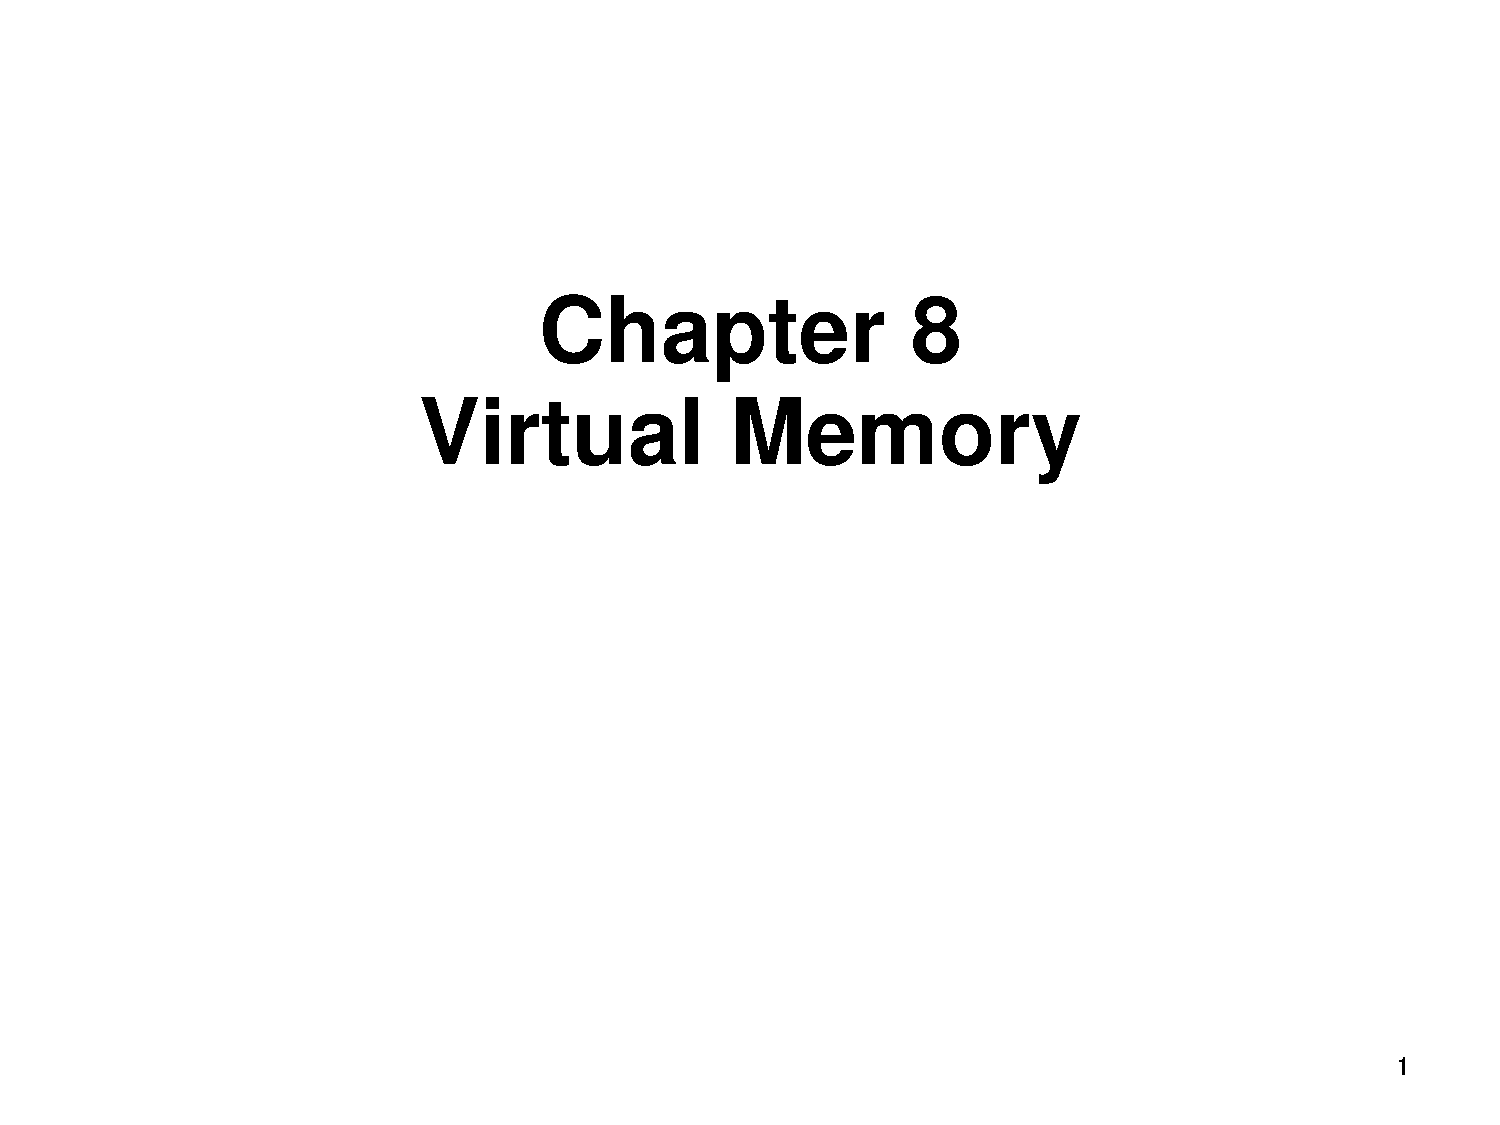
\includepdf[page=24]{08.pdf}
Each nested table takes the most significant bits as its key and copying over the rest to the next table. Works the same way as with regular paging, but with multiple levels. We can have page faults into root memory. We suspend the process while we load shit just like we do with single level paging. Here we have two ways to page fault (on root memory and main memory).

For every address we translate we need to access memory twice (once for memory and once for memory). This increases with multiple levels of paging.
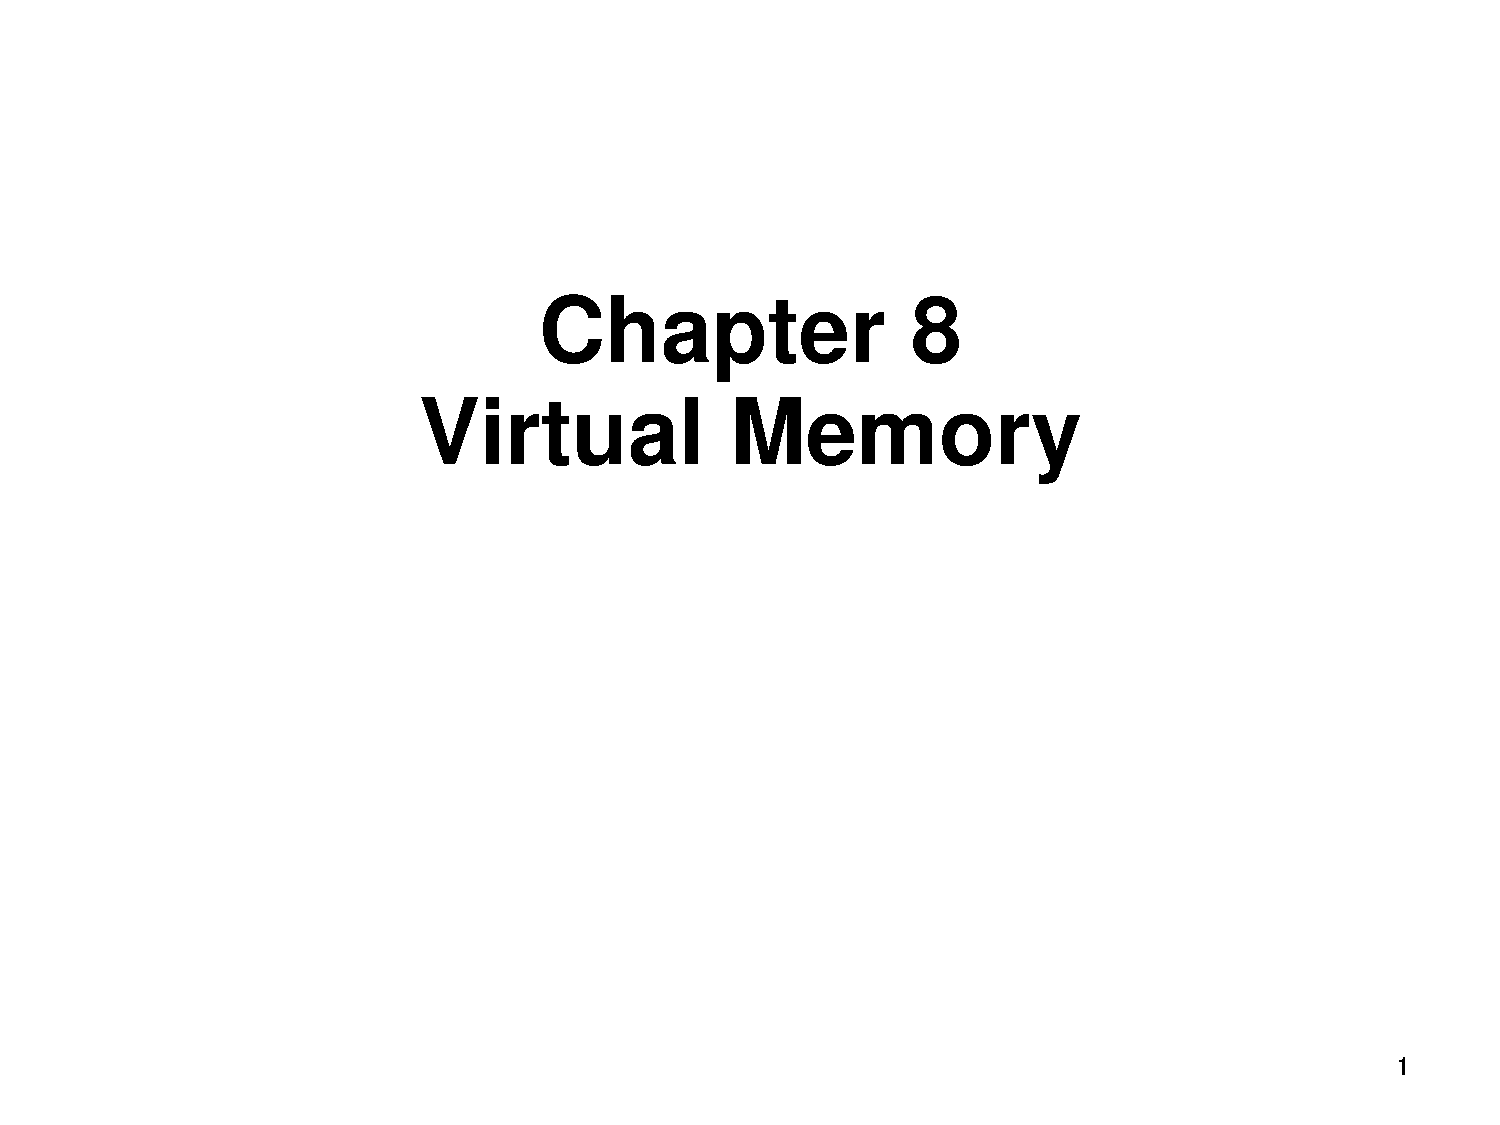
\includepdf[page=25]{08.pdf}
While we still have growth in our tables, but its much smaller (by number of bits). Page table size is proportional to address space, one page table per process.
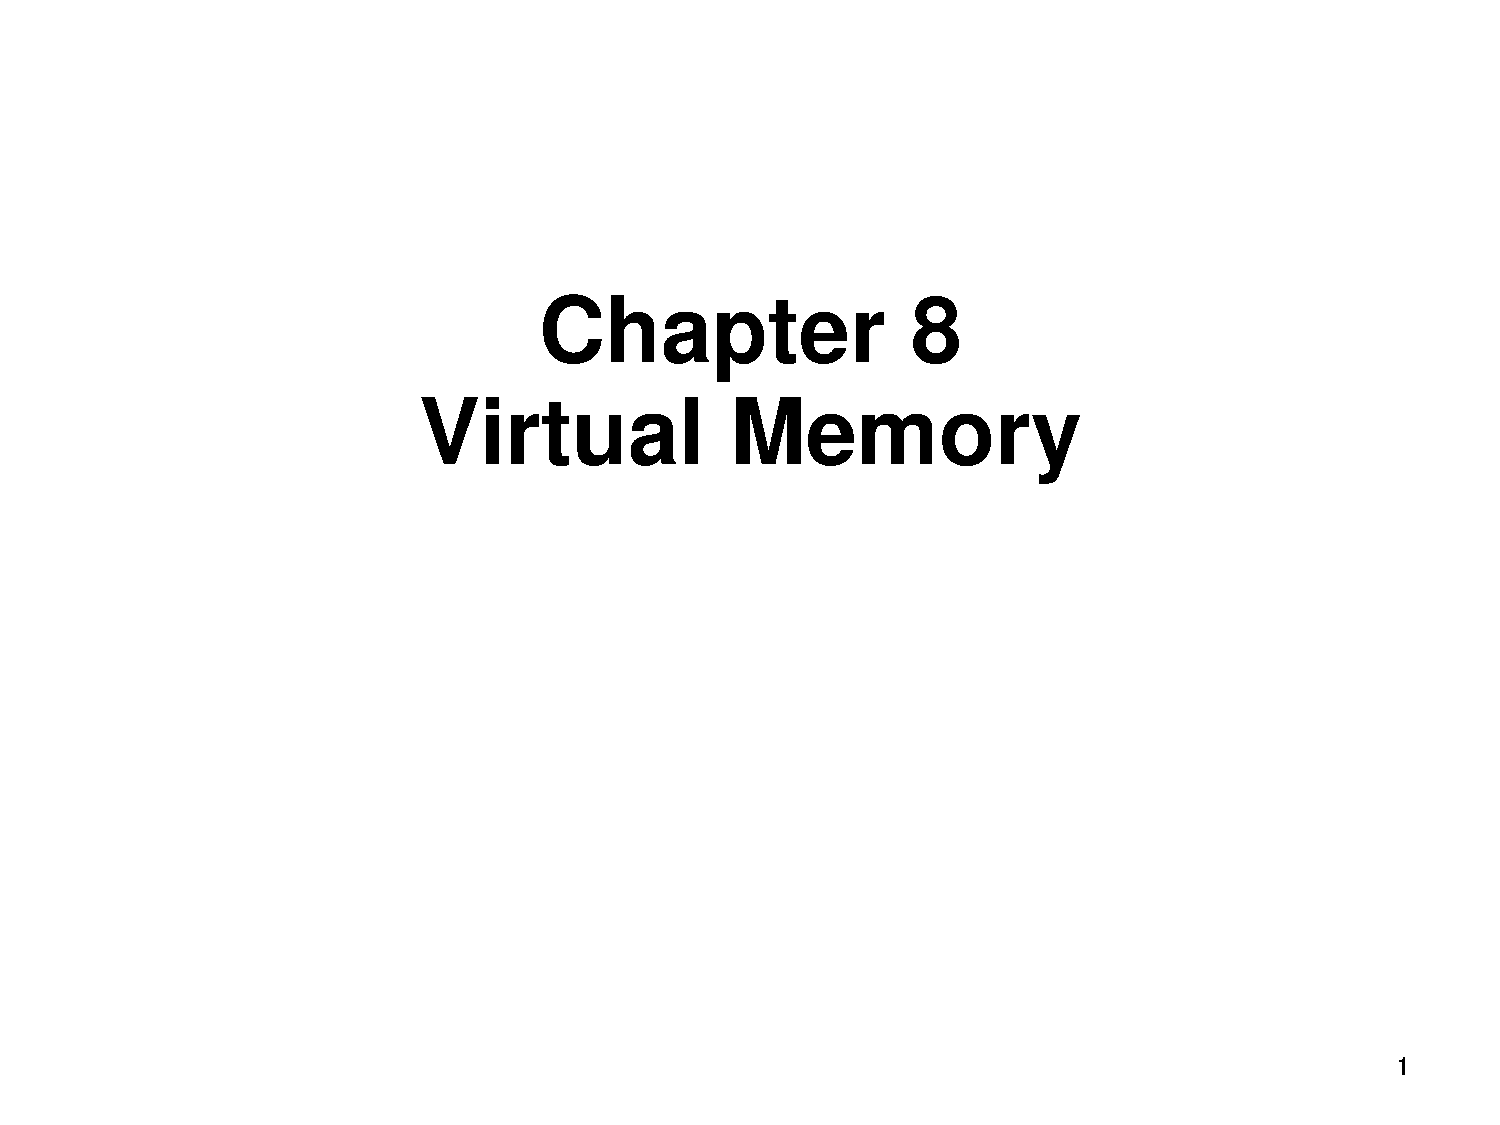
\includepdf[page=26]{08.pdf}
Go backwards from the frames into the page tables. Index the frames in our system and ensure that the index doesn't expand past our bounds of memory.
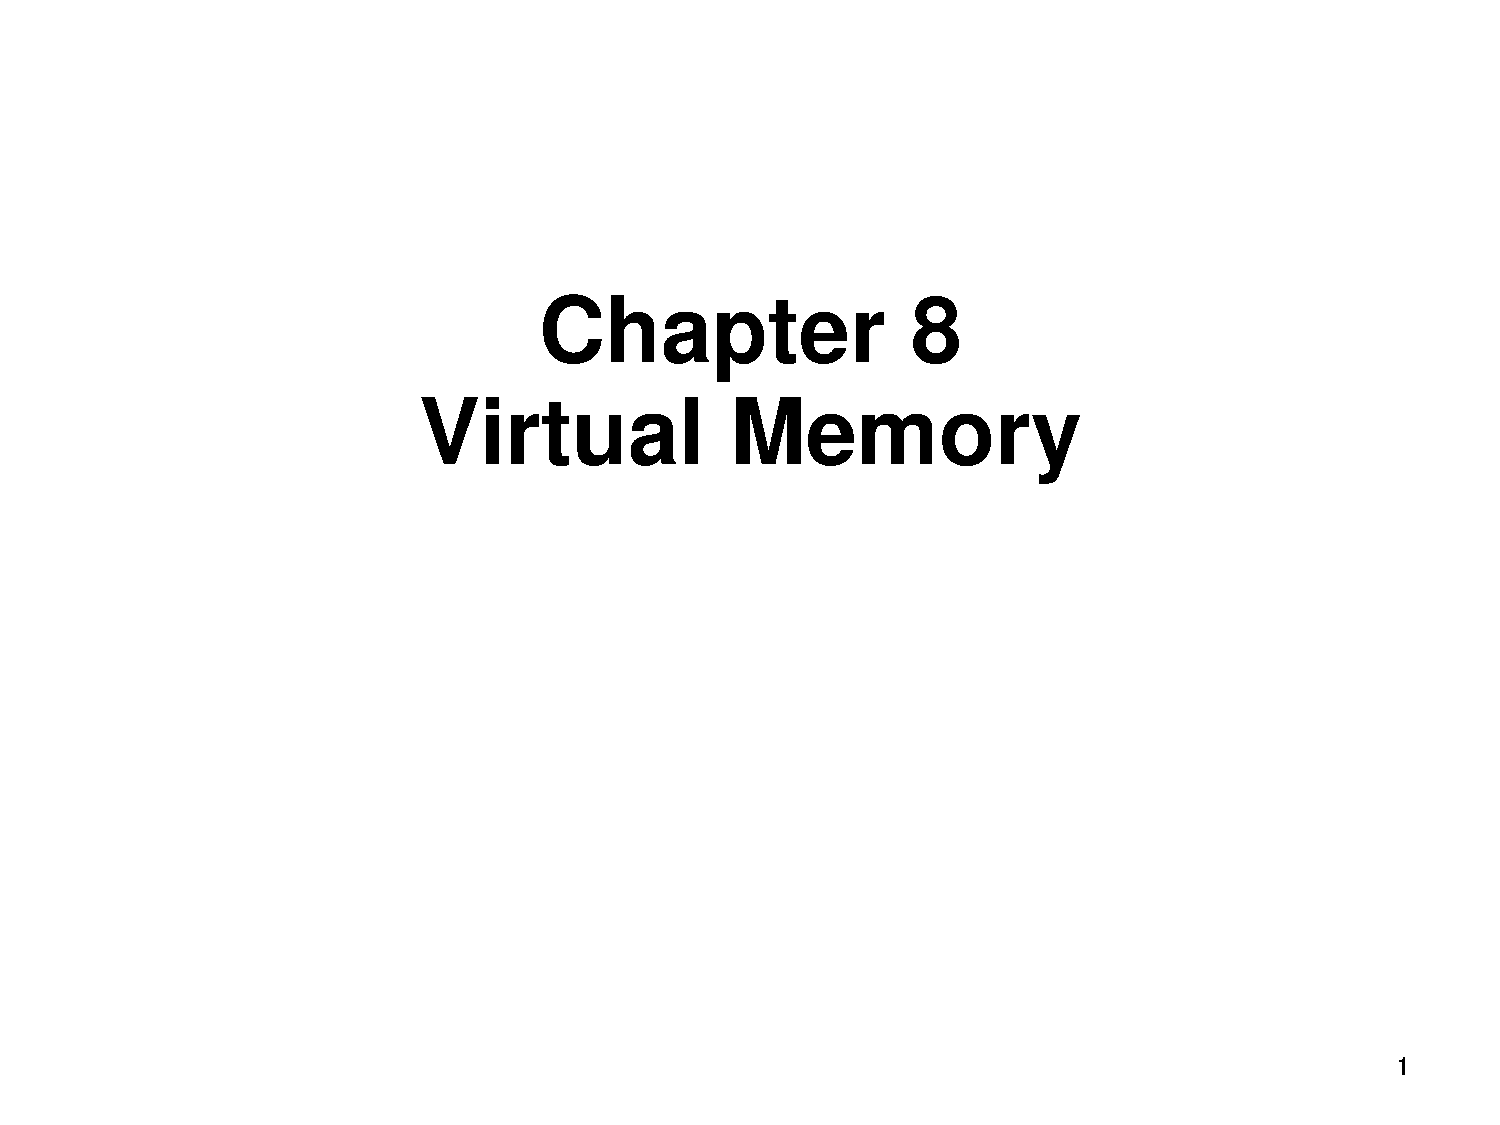
\includepdf[page=27]{08.pdf}
Start with your physical memory. Divide it into frames (simple paging). Find a mapping from the process image to the physical memory. That was how we did it previously. Now we want one table that maps frames to page tables (backwards to previously). Here the size of the inverted page table is bound by number of frames. We map using a hash function. Map frames from physical address through hash function into inverted page table.

We need to be able to detect collisions. Keep track of what process owns a frame and what page owns the frame.
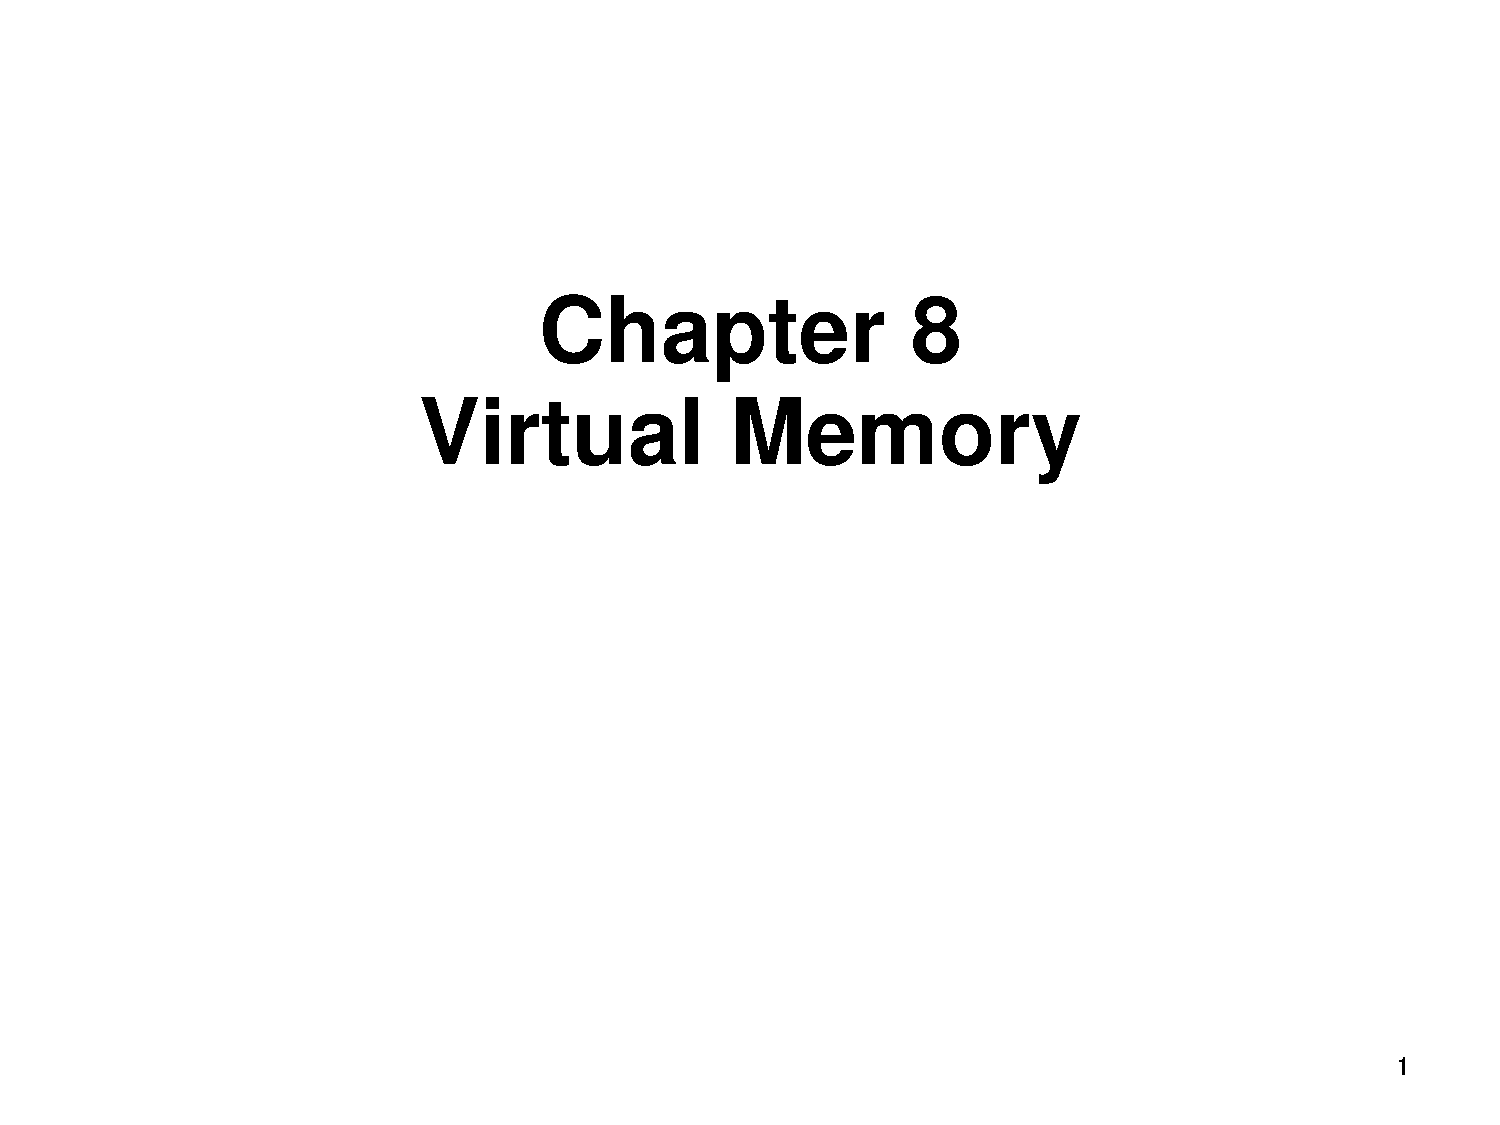
\includepdf[page=28]{08.pdf}
When our system becomes too slow (due to multiple memory accesses for paging) we add caches. We put this between the table and memory to increase look up speed. When we try to resolve a page number look at the cache and see if it has the page number. So we can pull from there instead of calculating before loading from memory. If we have a cache miss we load the address into there from main memory.

Instead of always trying to hit the page table we cache page table entries in a cache, basically.
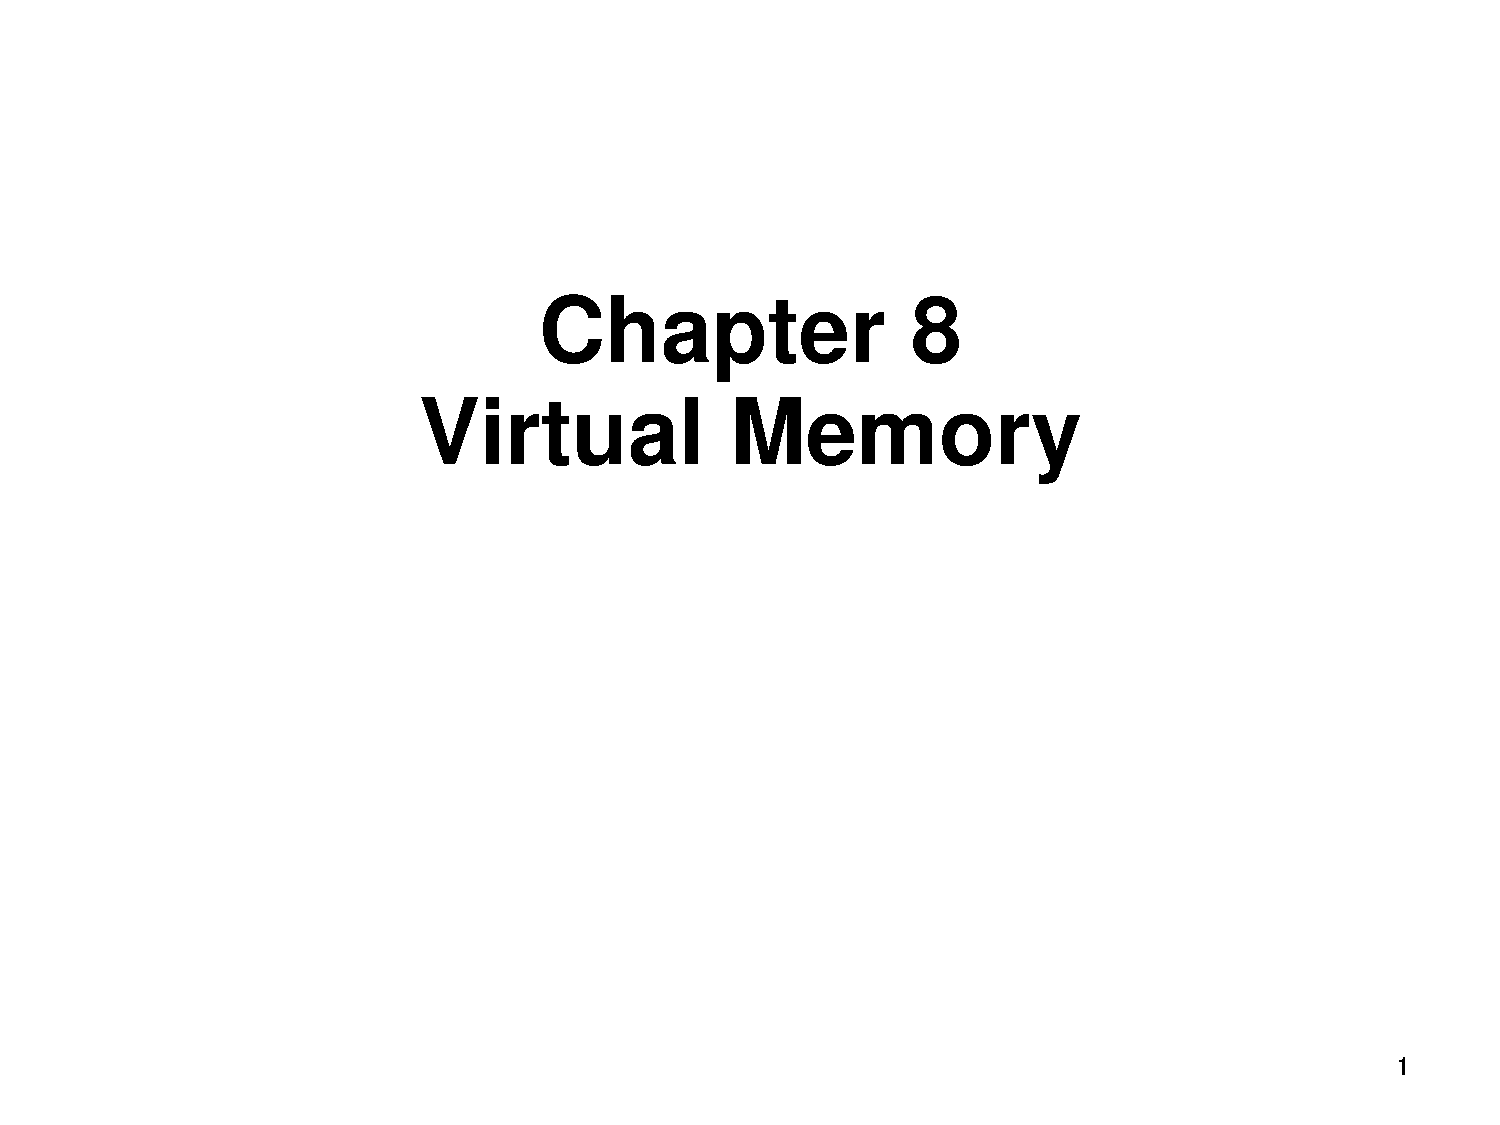
\includepdf[page=29]{08.pdf}
When we preform a context switch between processes we have to dump the whole TLB (its only accurate for the currently running process). We could also maintain the TLB as some house keeping and load it during switch. The norm is to just flush the TLB during switches.
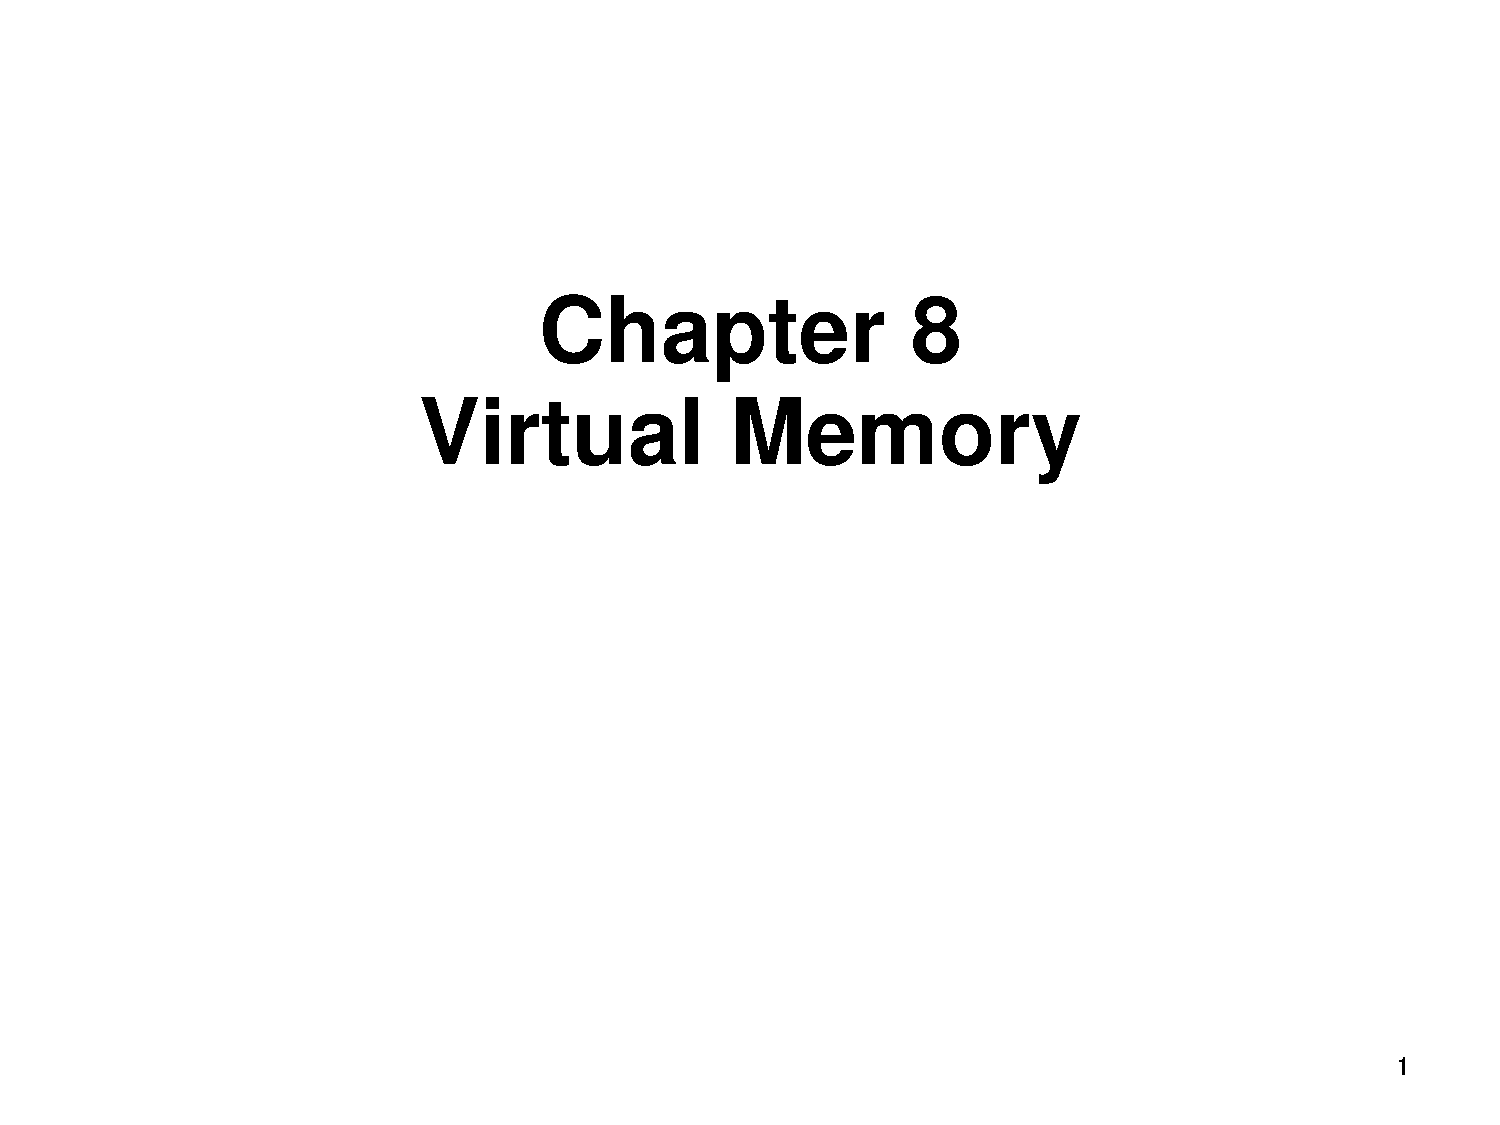
\includepdf[page=30]{08.pdf}
Check TLB to see if the page table is there and we can generate the address automatically. If it is not we go to page table and fetch the page number and load it into the TLB. If the page is not in main memory we get a page fault and have to go look shit up.
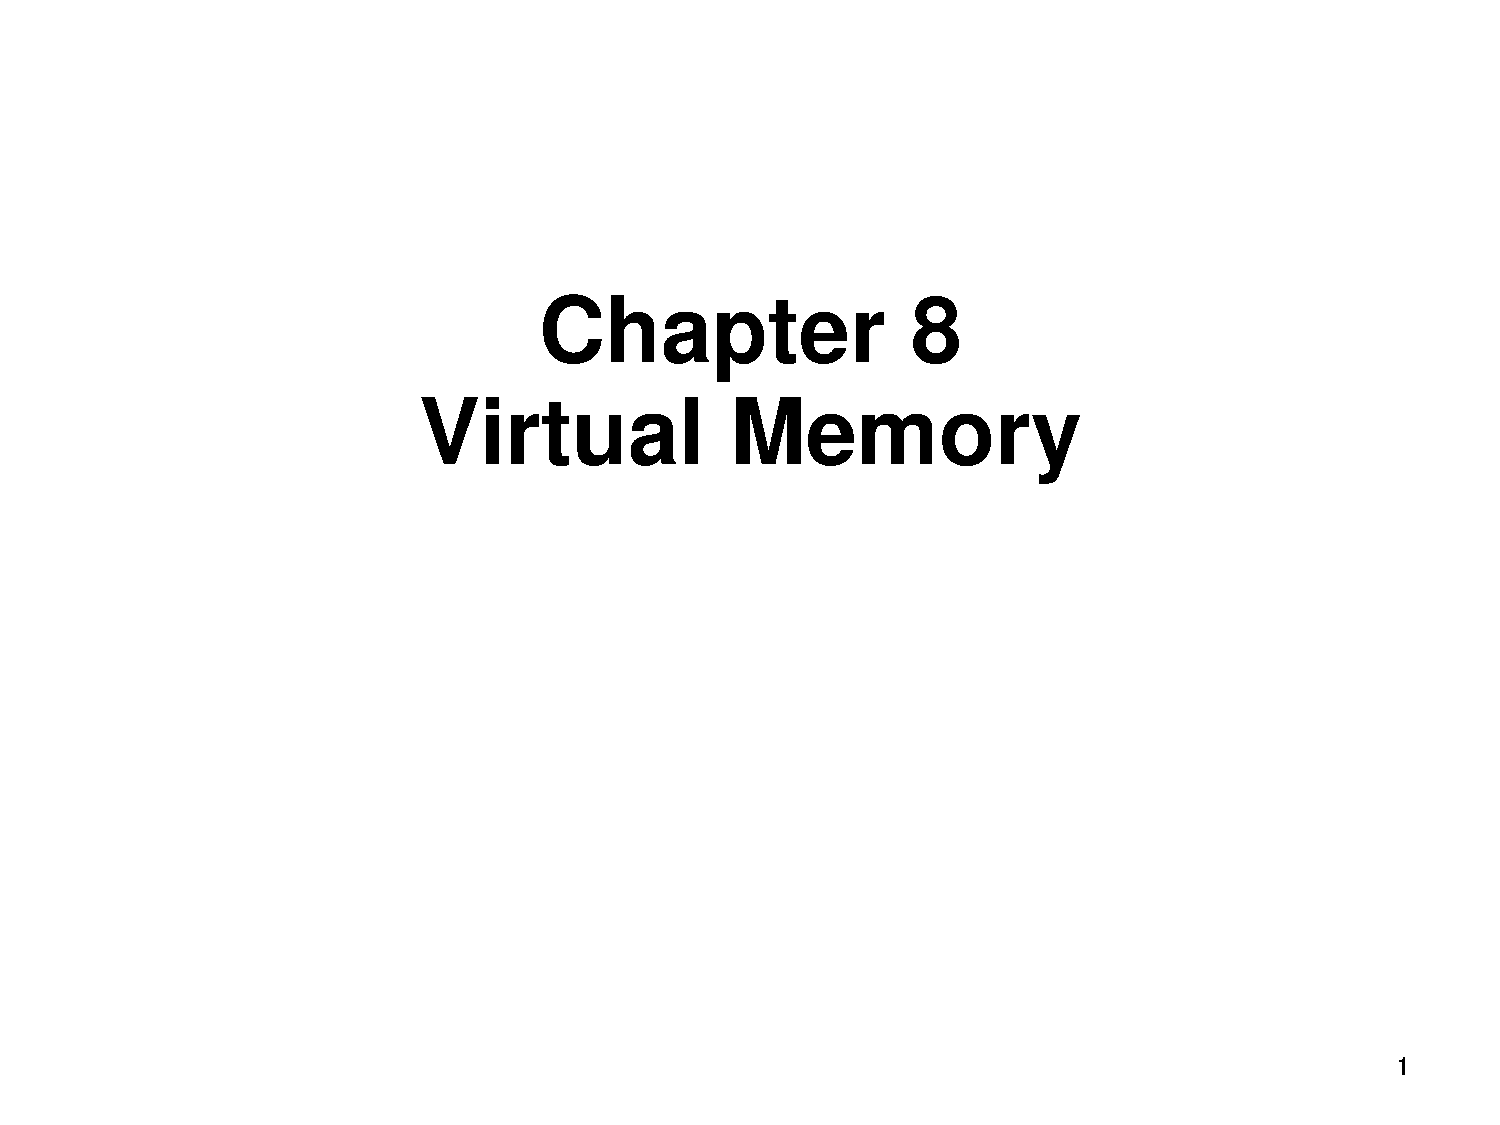
\includepdf[page=31]{08.pdf}
We need to do an associate mapping between addresses. This is not a linear index (which the page table uses). Basically hash that shit.
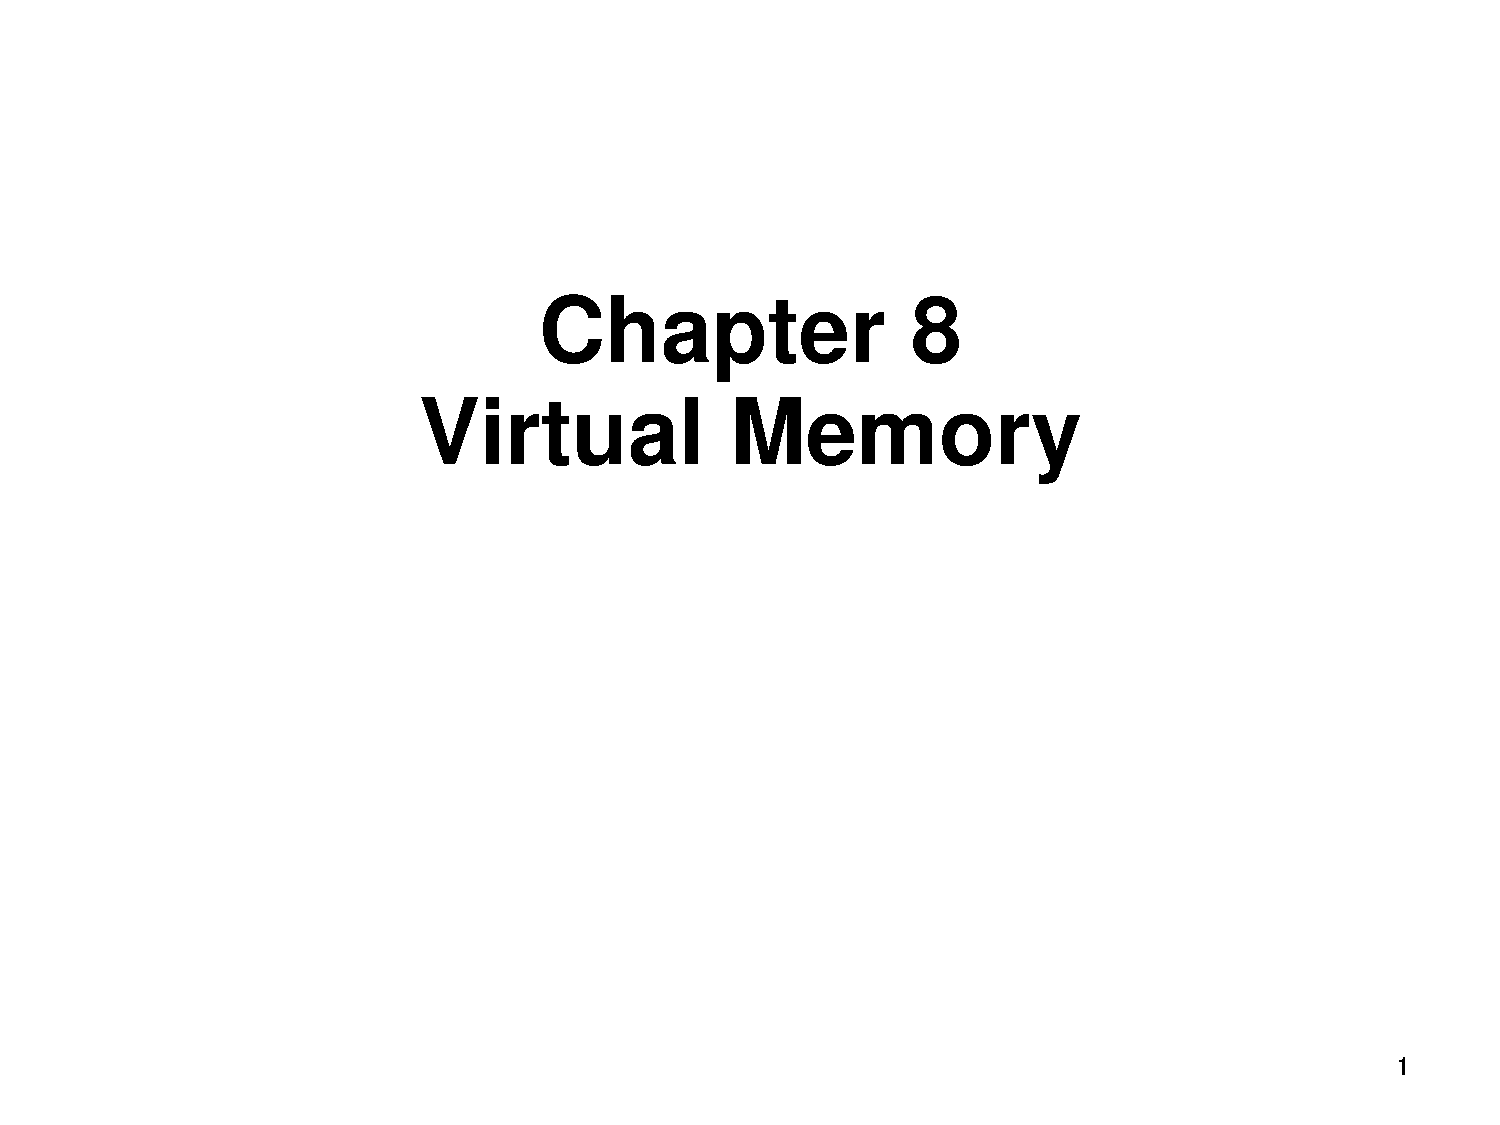
\includepdf[page=32]{08.pdf}
Here we split everything up into systems. We have the TLB look up operation. When we have a miss we go to memory and resolve the page table. Once we hav the physical address we have the cache operation
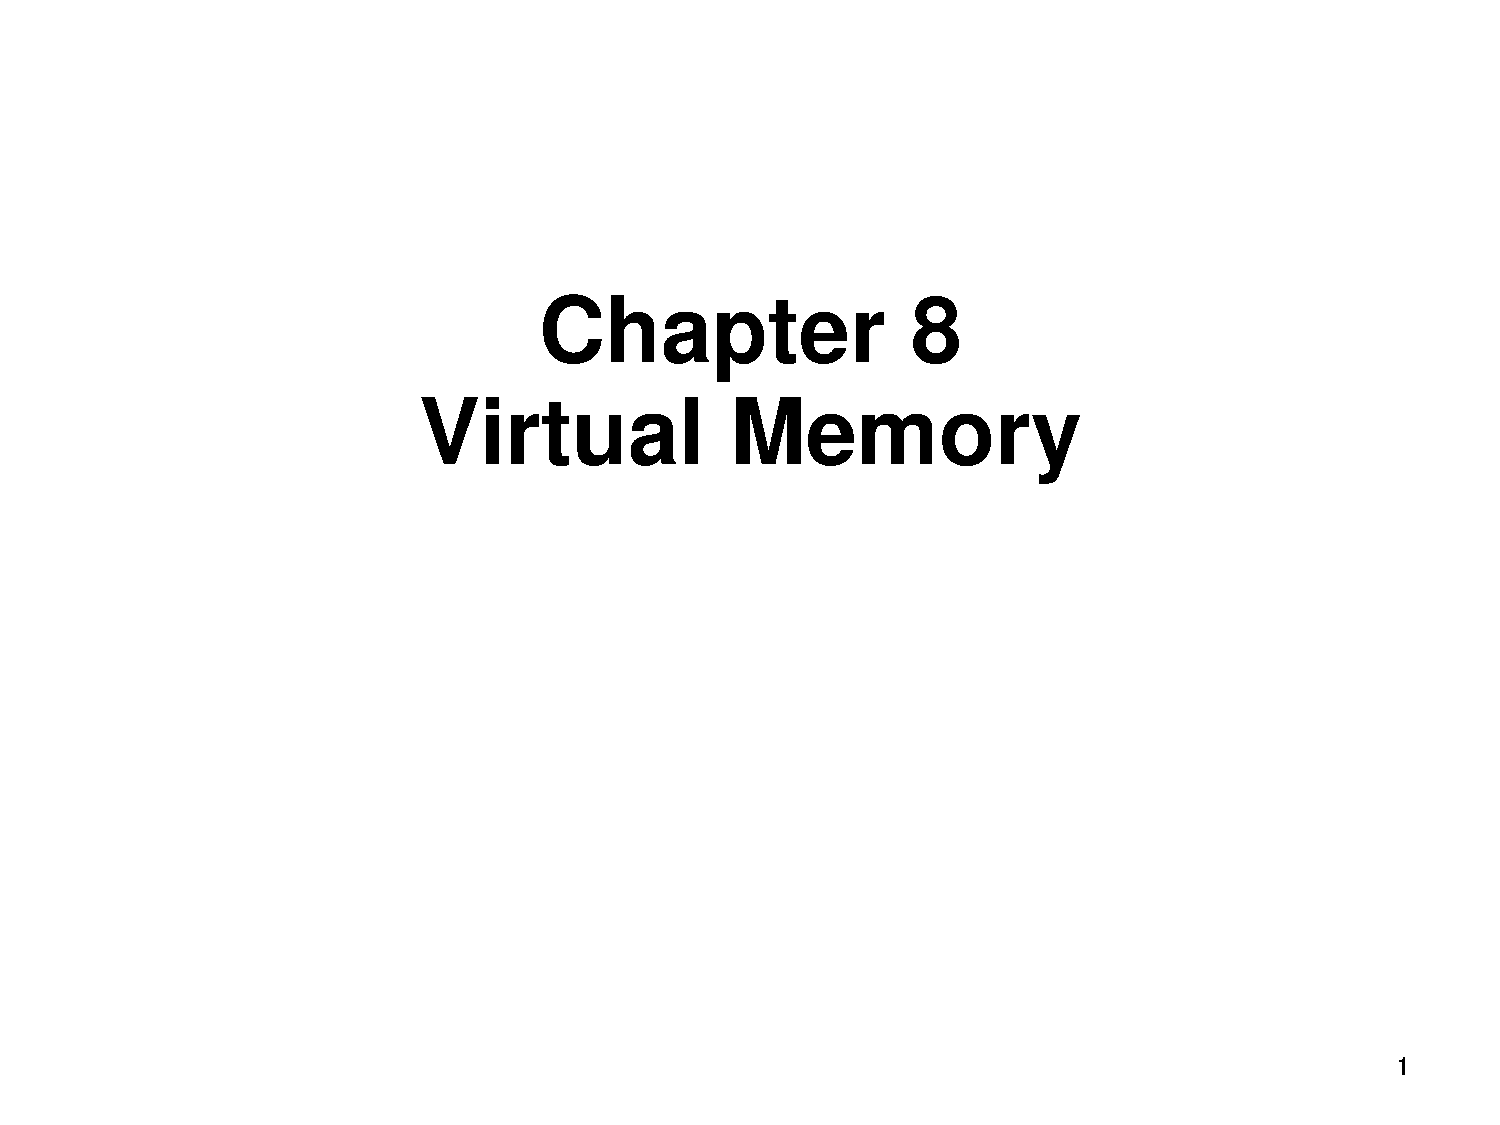
\includepdf[page=33]{08.pdf}
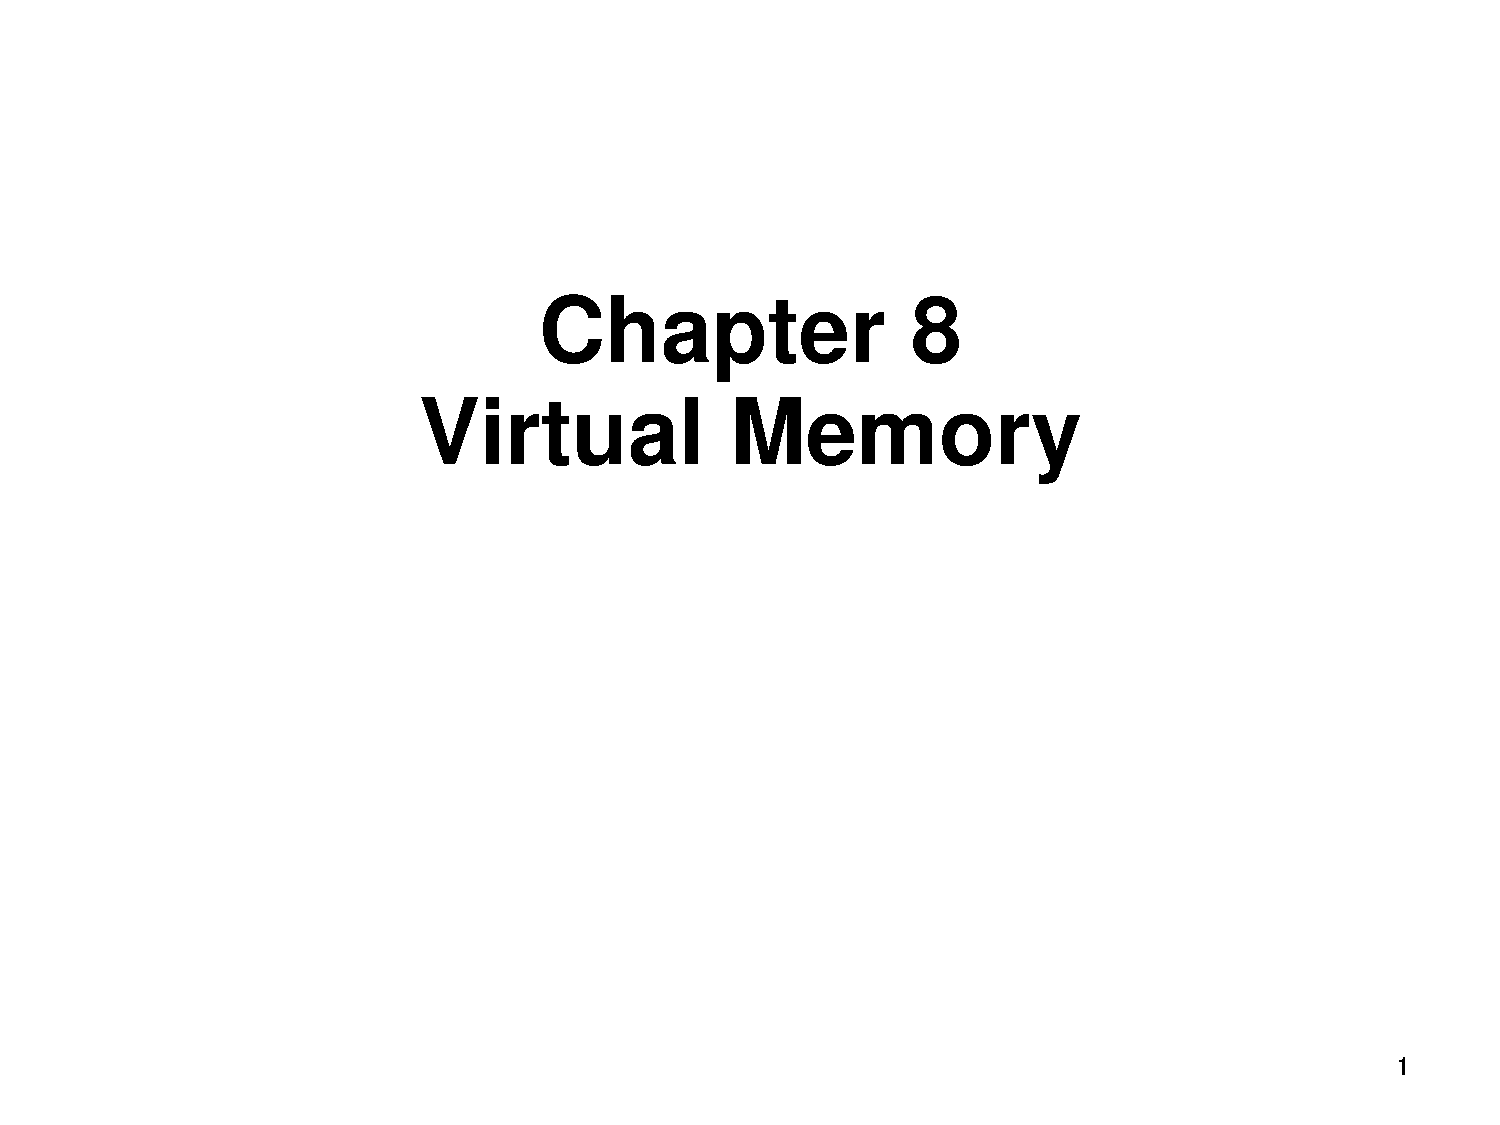
\includepdf[page=34]{08.pdf}
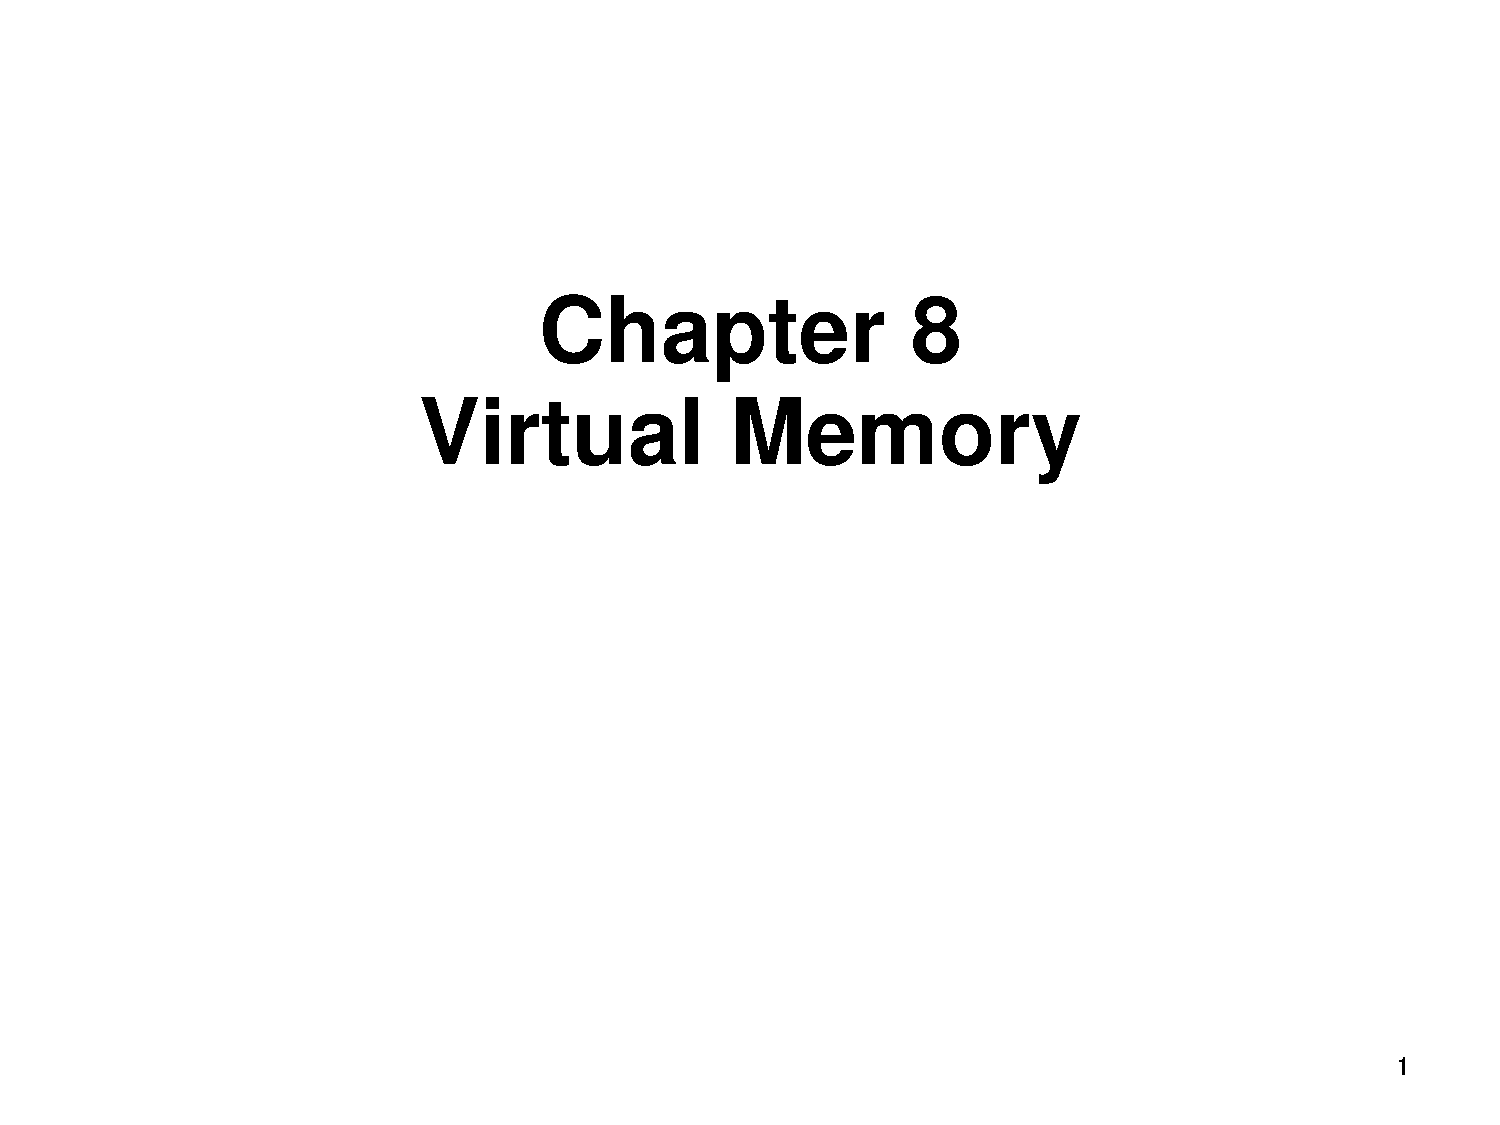
\includepdf[page=35]{08.pdf}
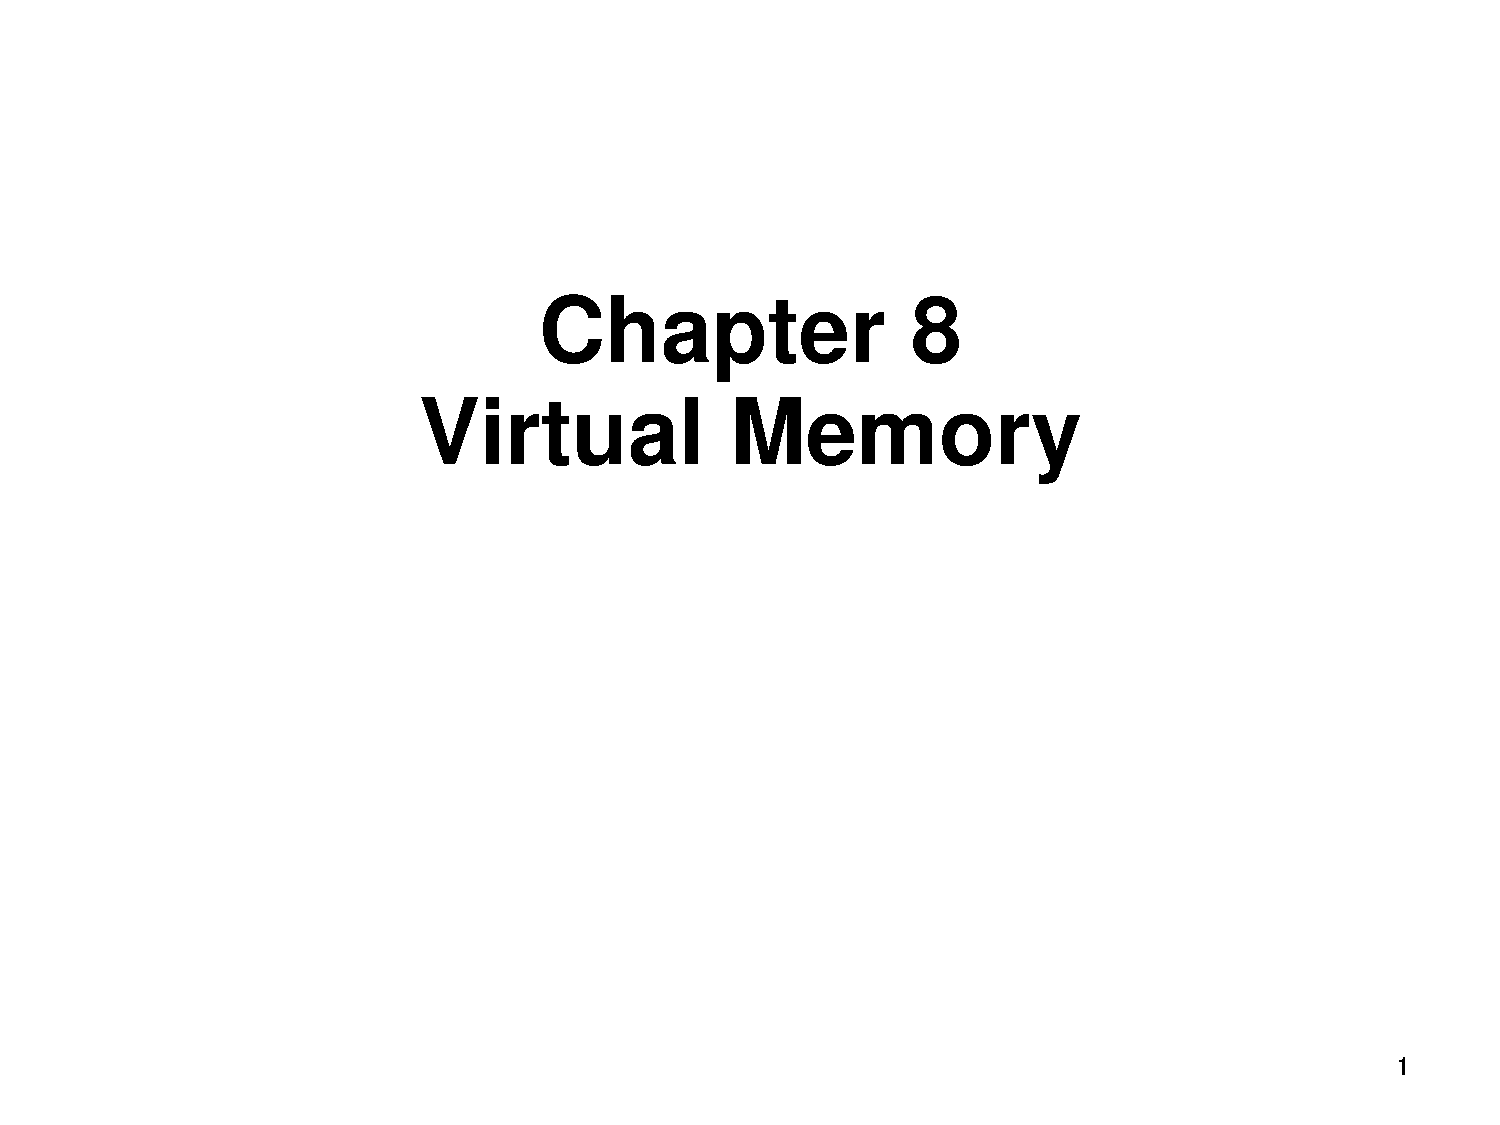
\includepdf[page=36]{08.pdf}
This is a much more complicated topic, we come back to it laters. The working set becomes important for replacement policies.
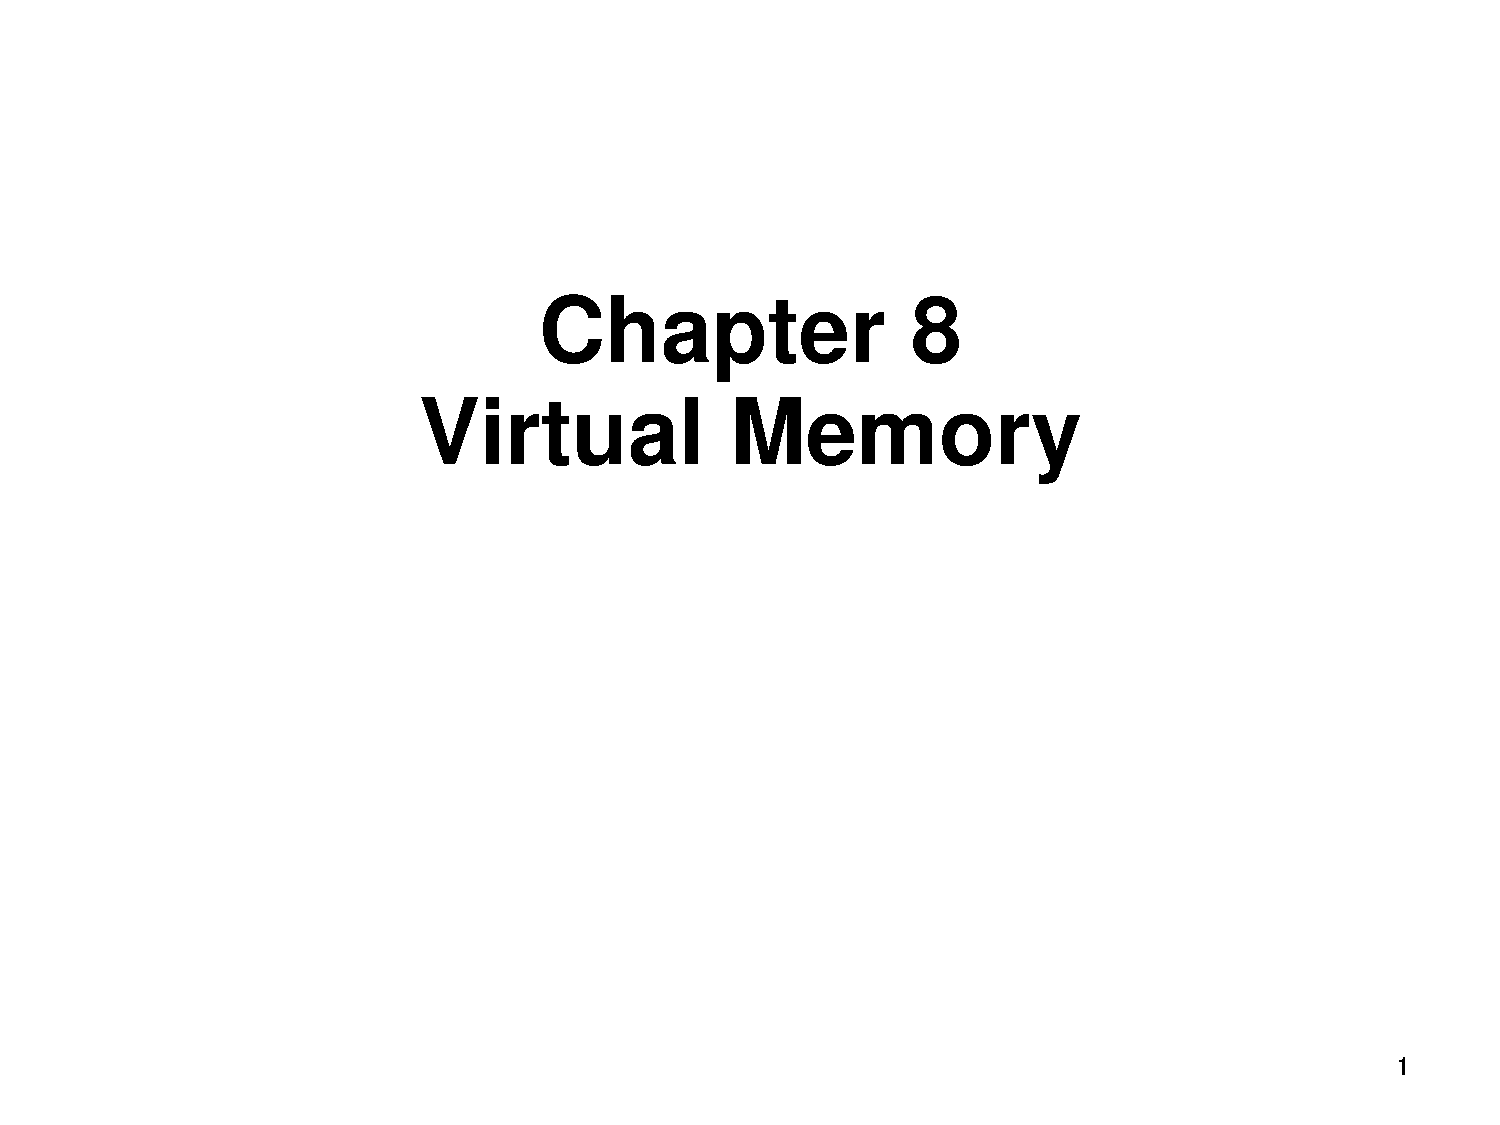
\includepdf[page=37]{08.pdf}
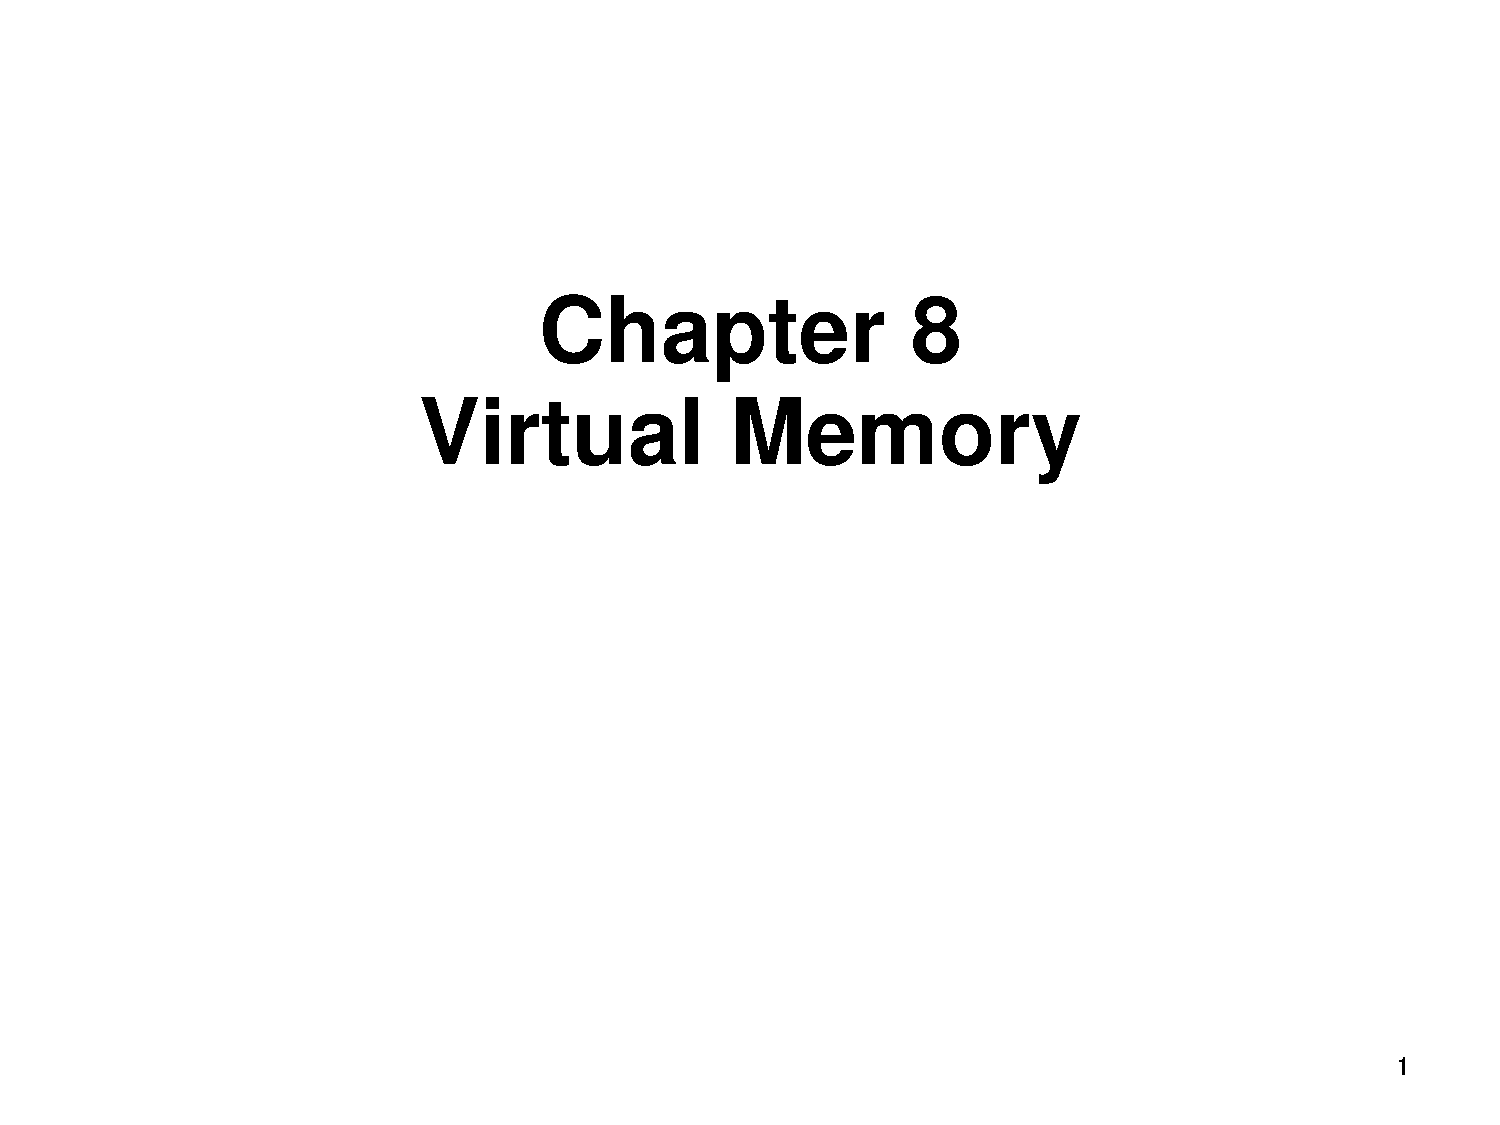
\includepdf[page=38]{08.pdf}
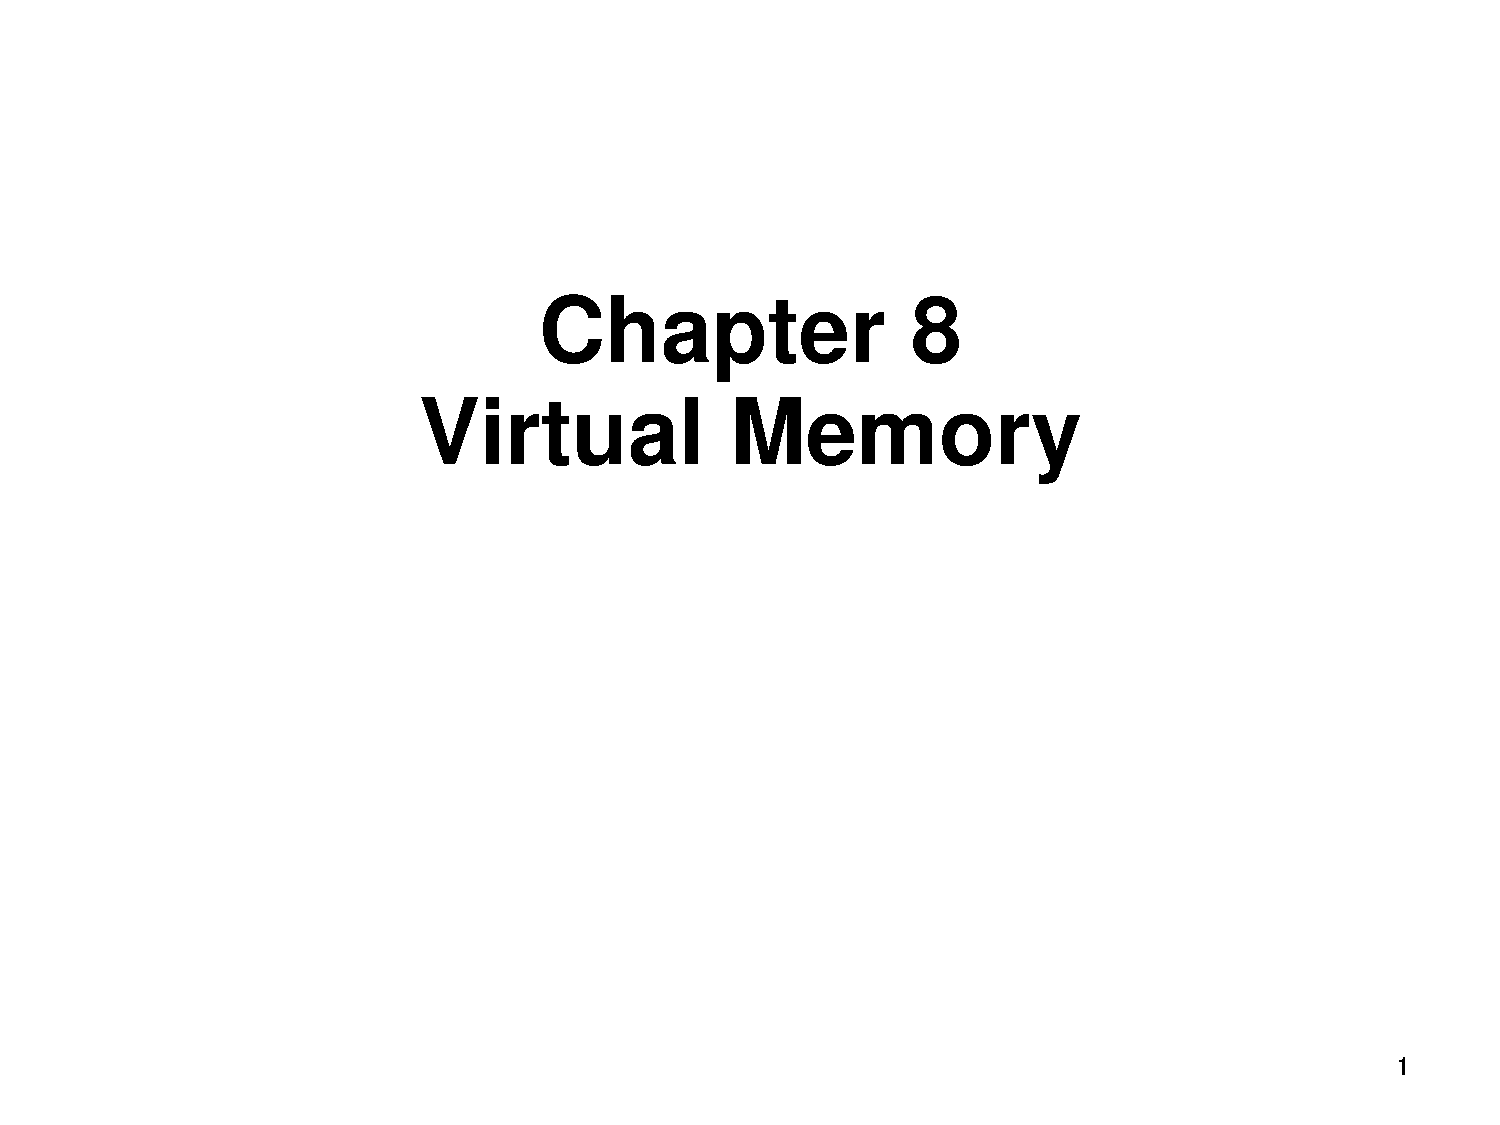
\includepdf[page=39]{08.pdf}
Here we allow processes to be compiled independantly (linking). Veriable size blocks allow us to independently protect so we can have process sharing. Use segmentation on our virtual memory management scheme.
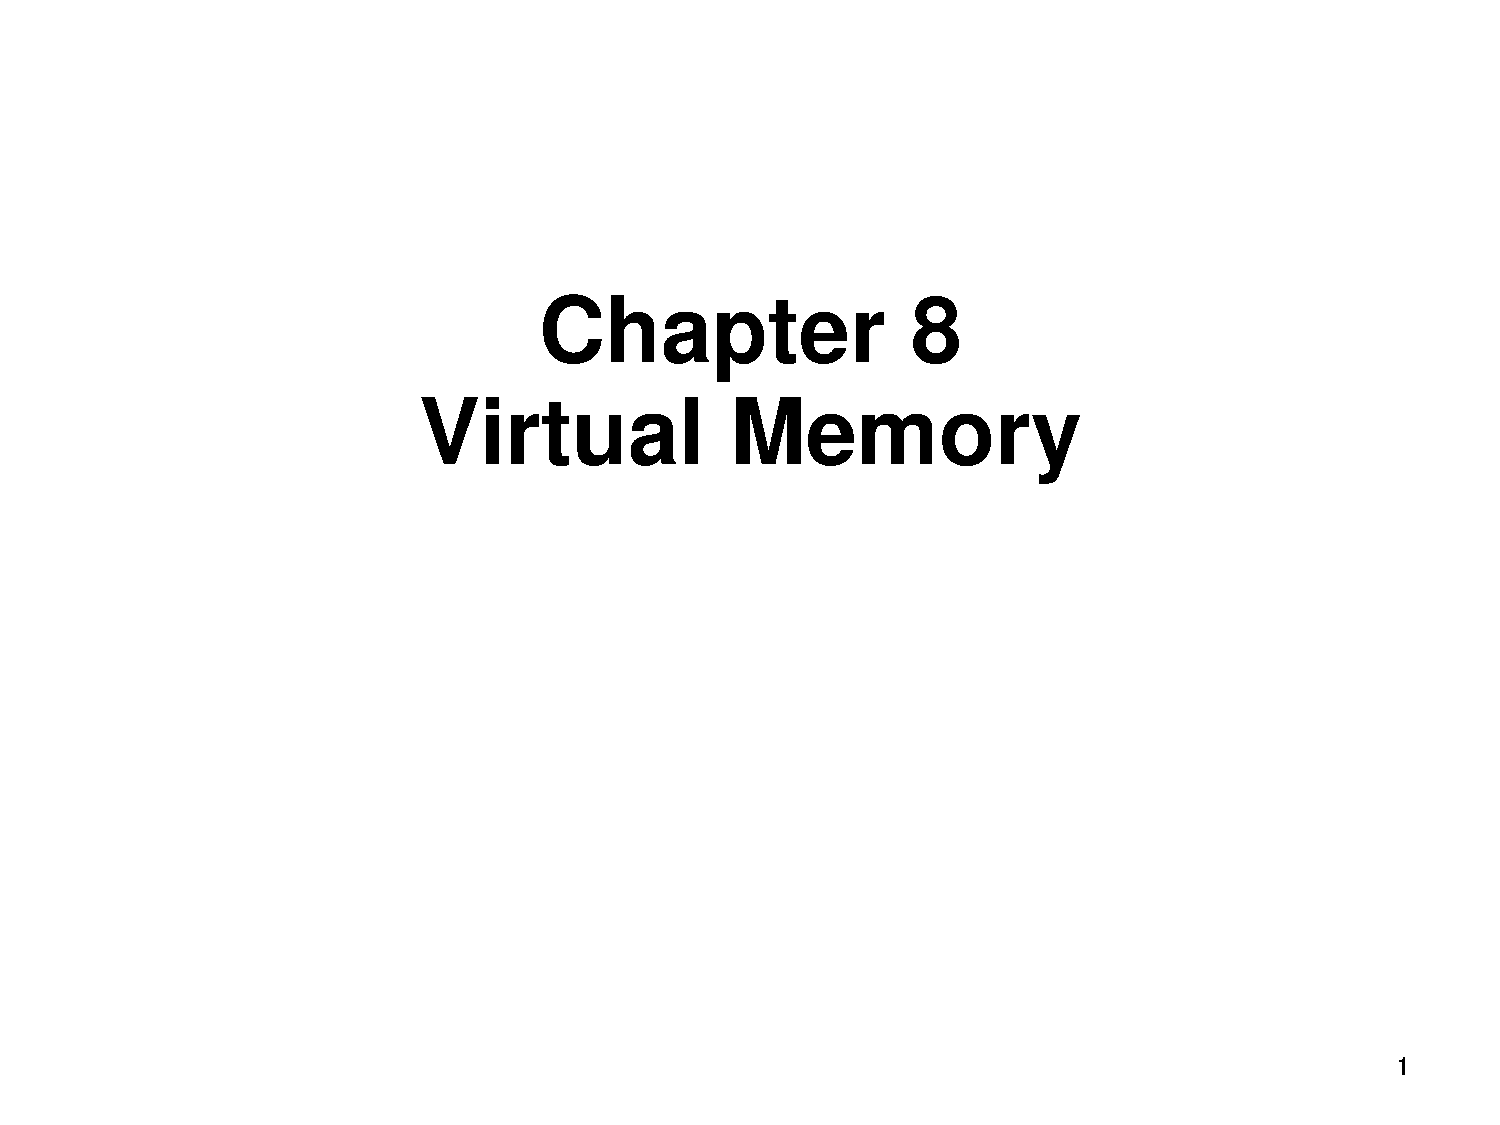
\includepdf[page=40]{08.pdf}
Use segment tables to convert real address to virtual address. Need starting address and the length of the segment (also some housekeeping bits to know if the segment is in memory or has been modified).
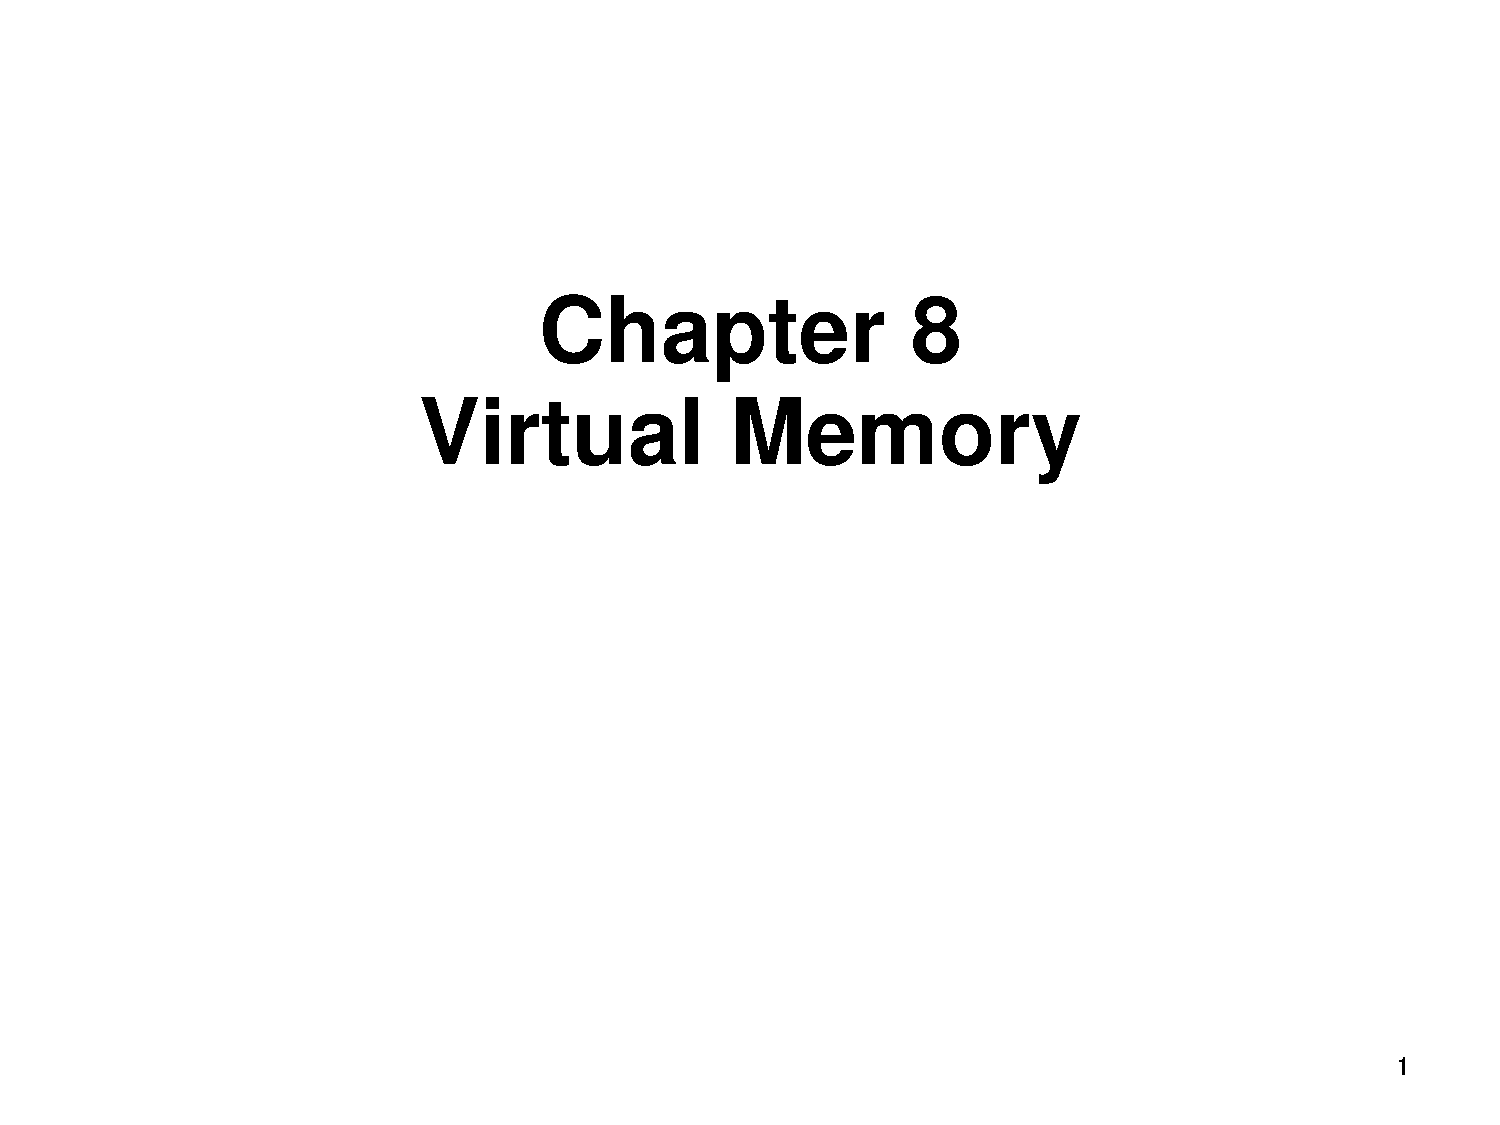
\includepdf[page=41]{08.pdf}
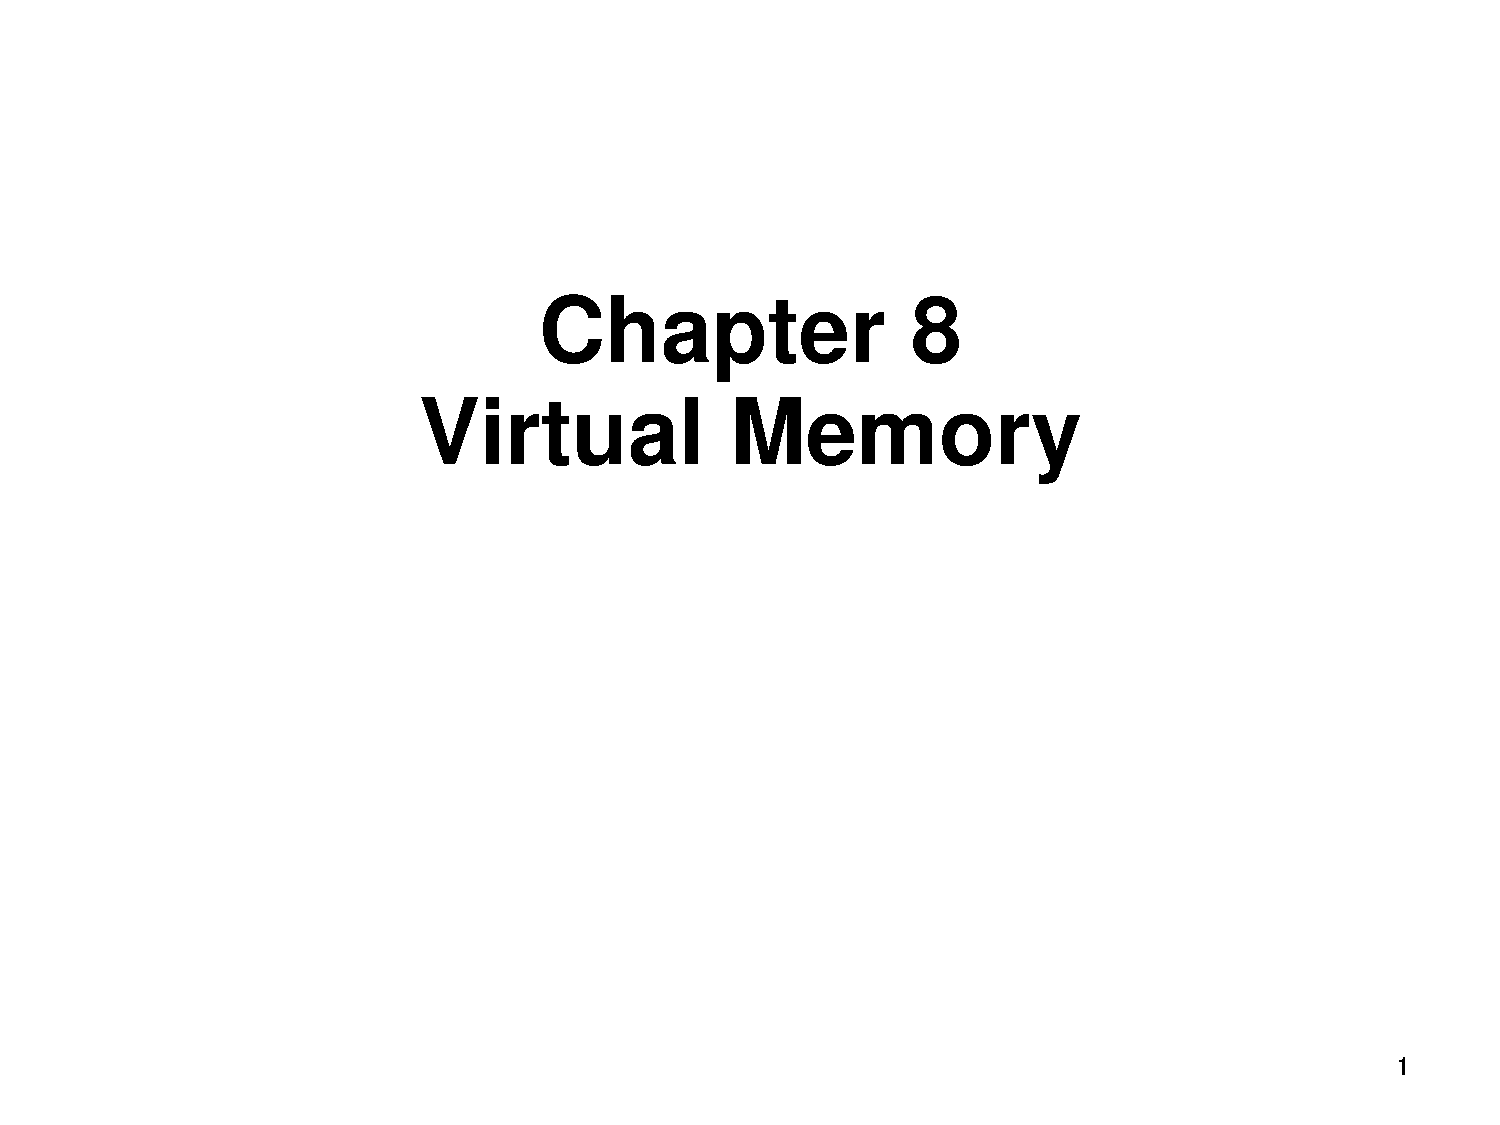
\includepdf[page=42]{08.pdf}
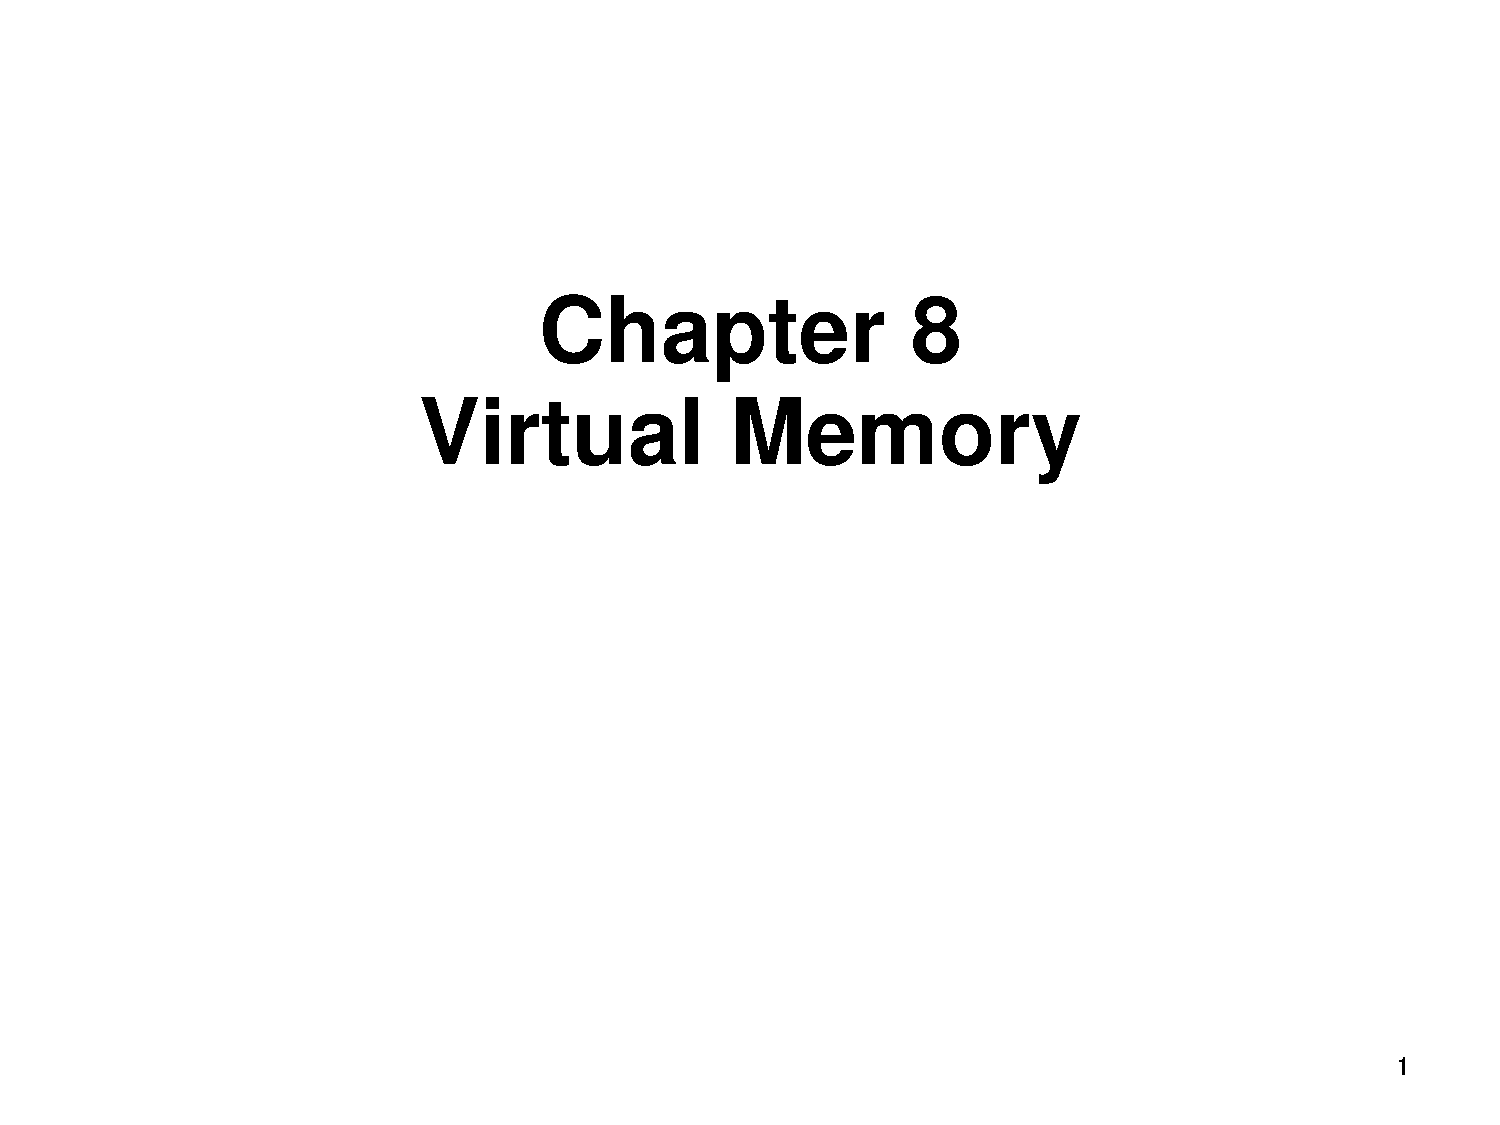
\includepdf[page=43]{08.pdf}
We want the user to be able to access segmentation because we want a modularized program that the user links together at compile time.
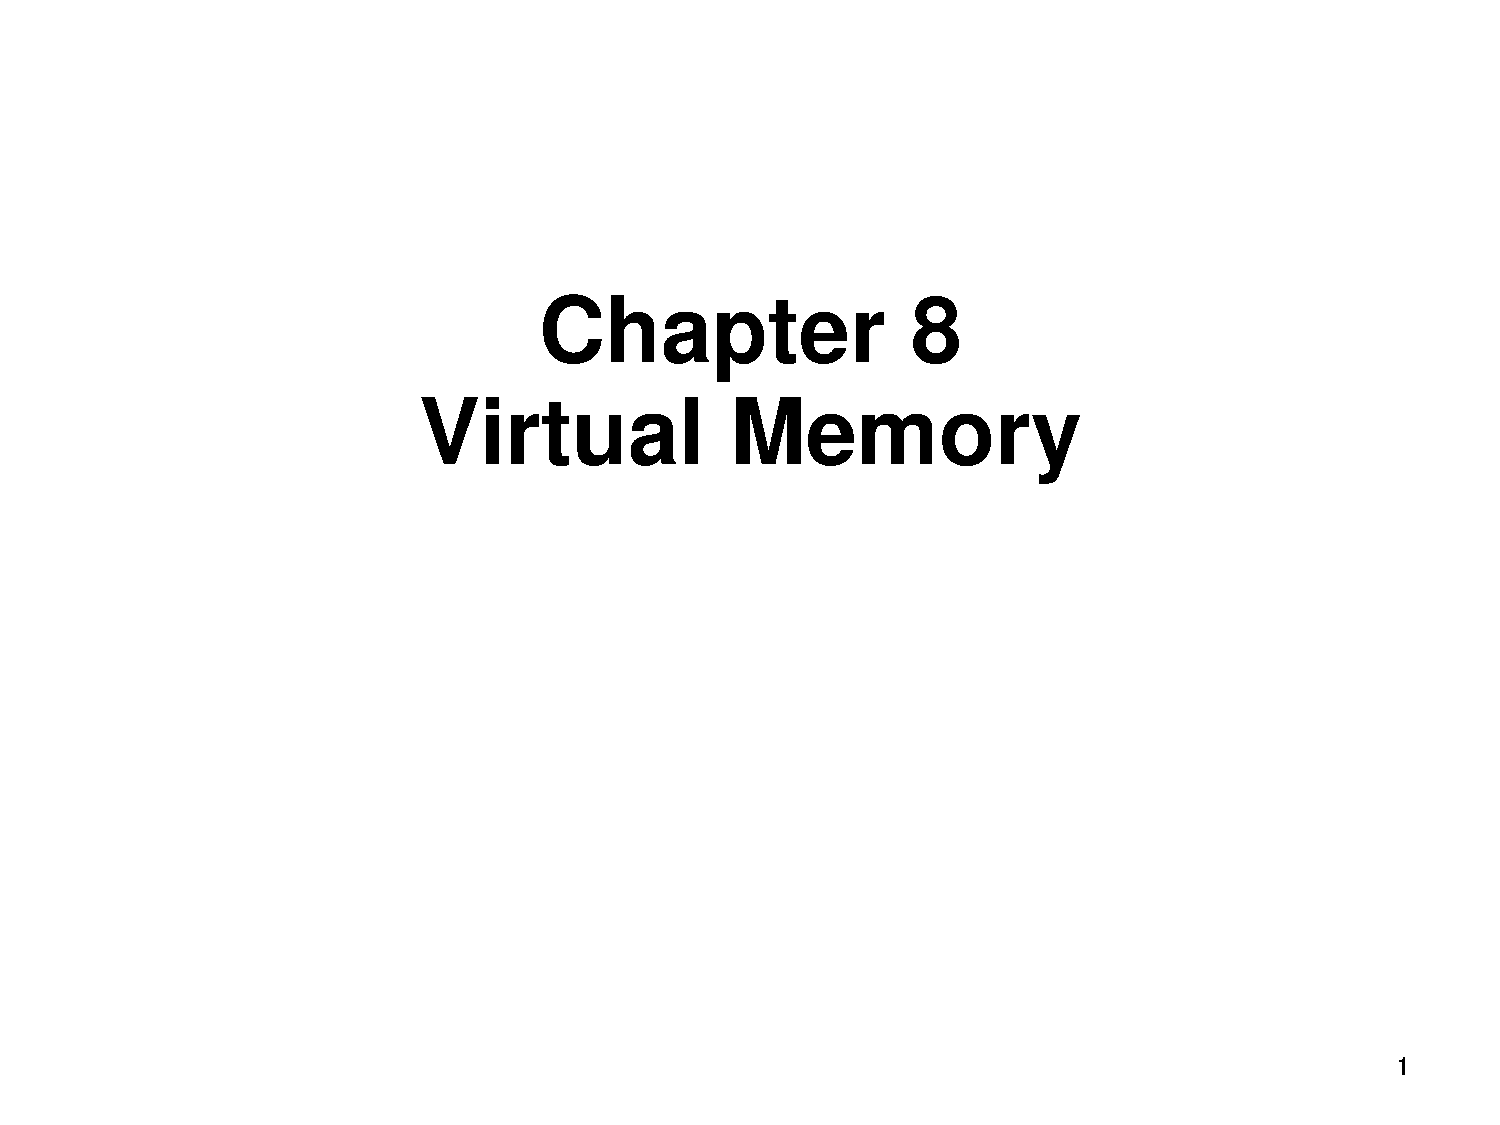
\includepdf[page=44]{08.pdf}
Have the segment number and break the offest apart into a page number and page offset. And some other shit he said too quickly.
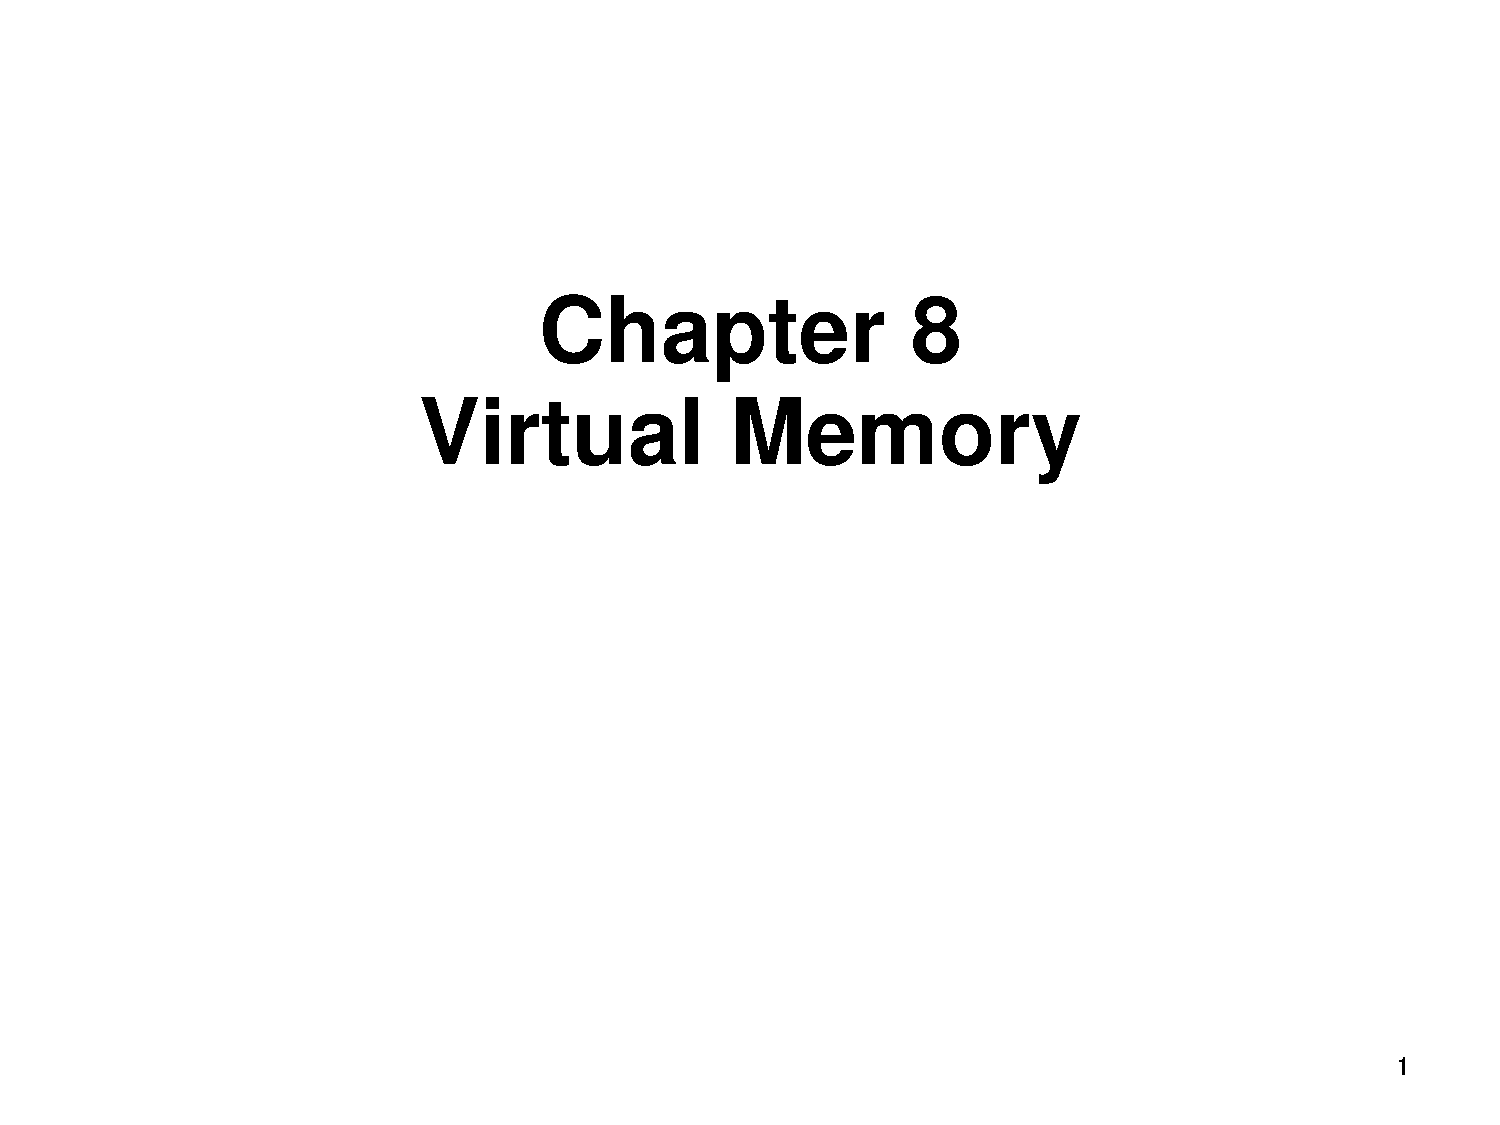
\includepdf[page=45]{08.pdf}
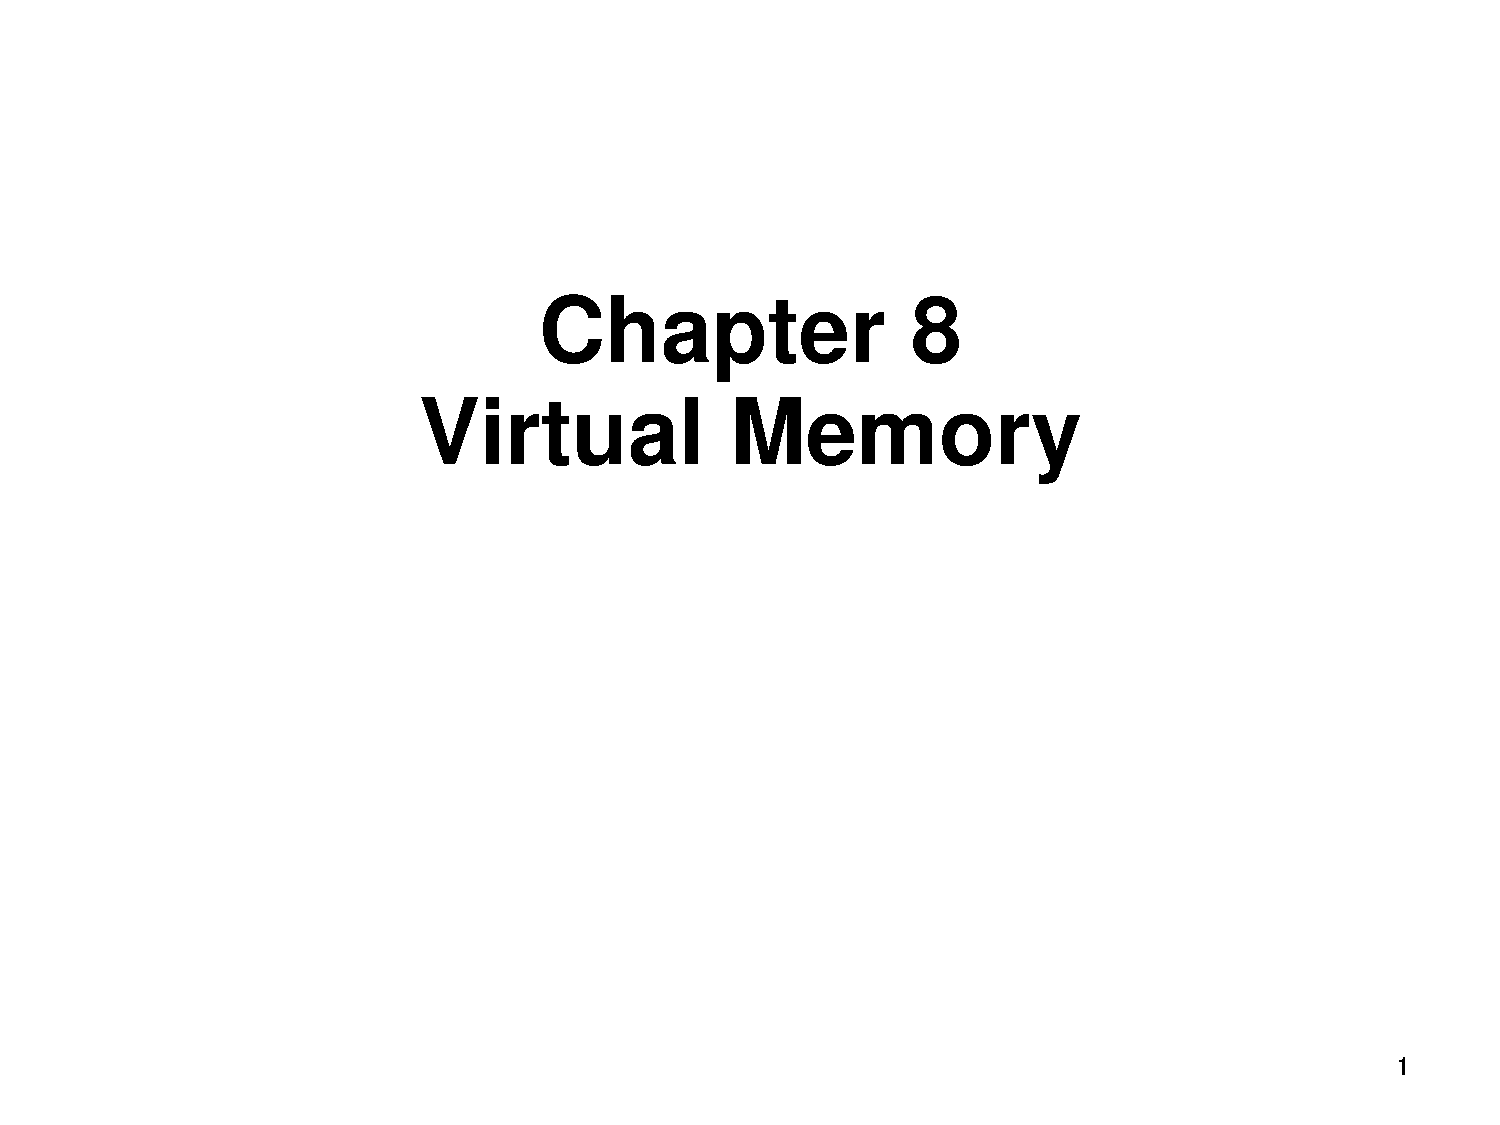
\includepdf[page=46]{08.pdf}
We can allow or disable branching to or from certain addresses. We can also allows restricted access to a processes memory. We need a way to protect these things. This is done with protection bits (read, write, execute, etc)
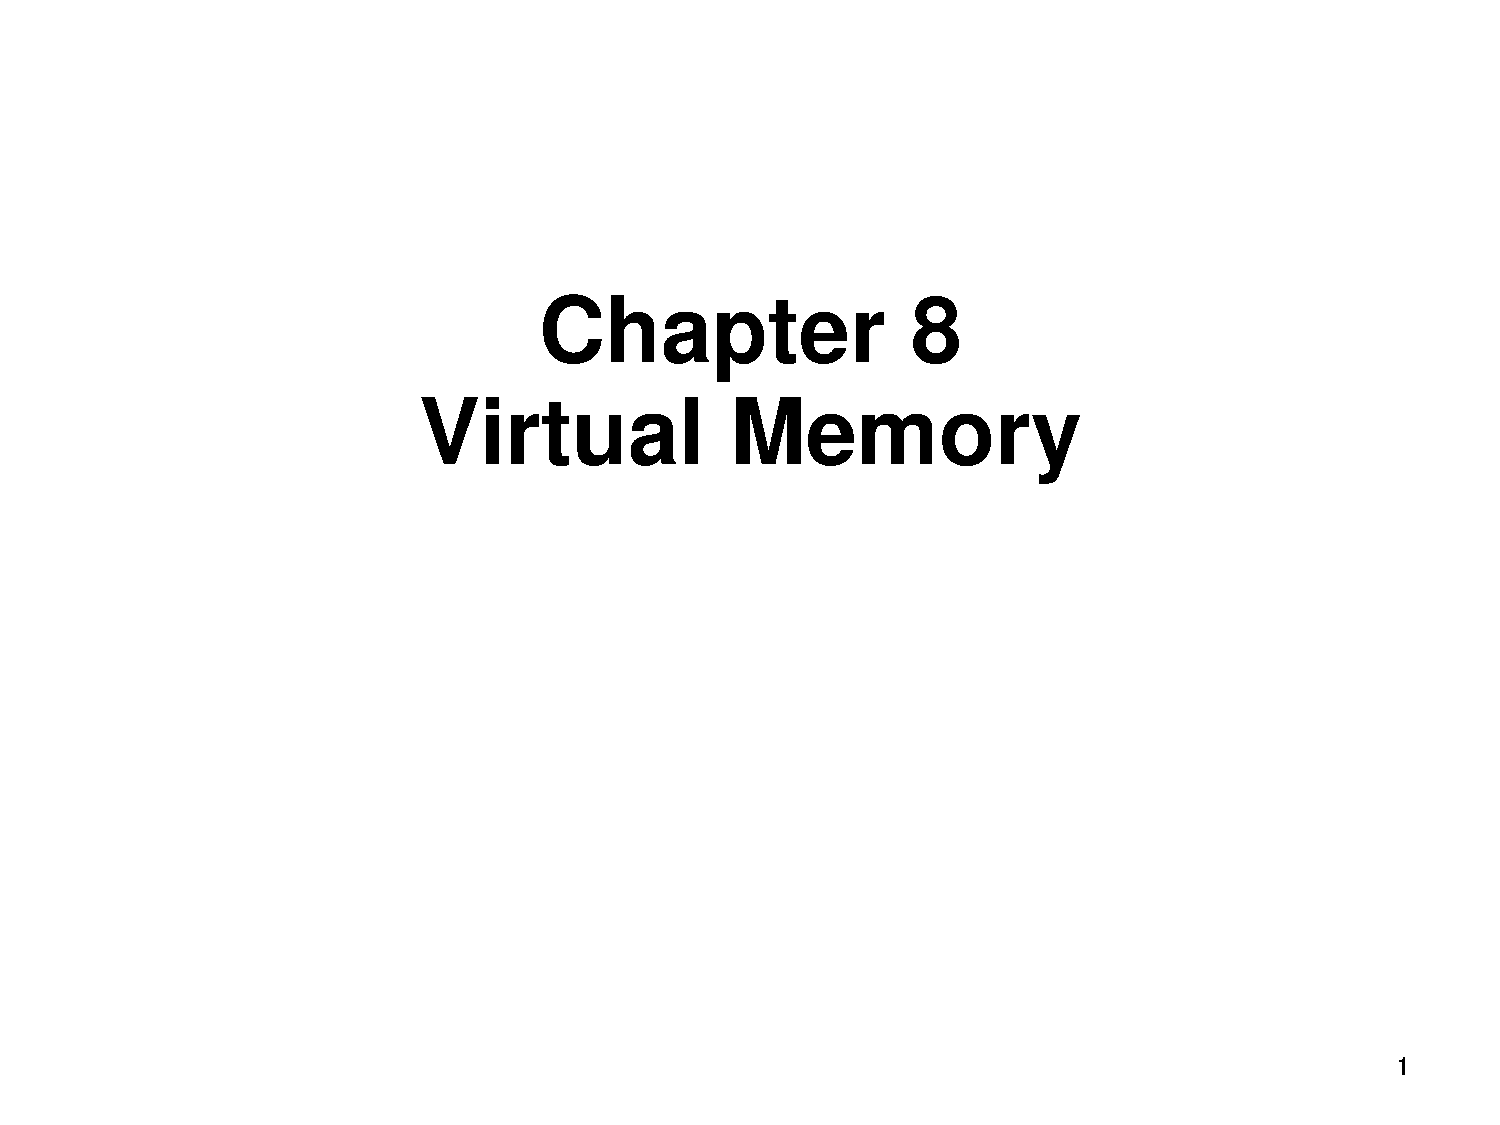
\includepdf[page=47]{08.pdf}
Usually we want both (segmentation for fine tuned control, paging for large memory). We will also need to decide how we moving things about through a series of algorithms.
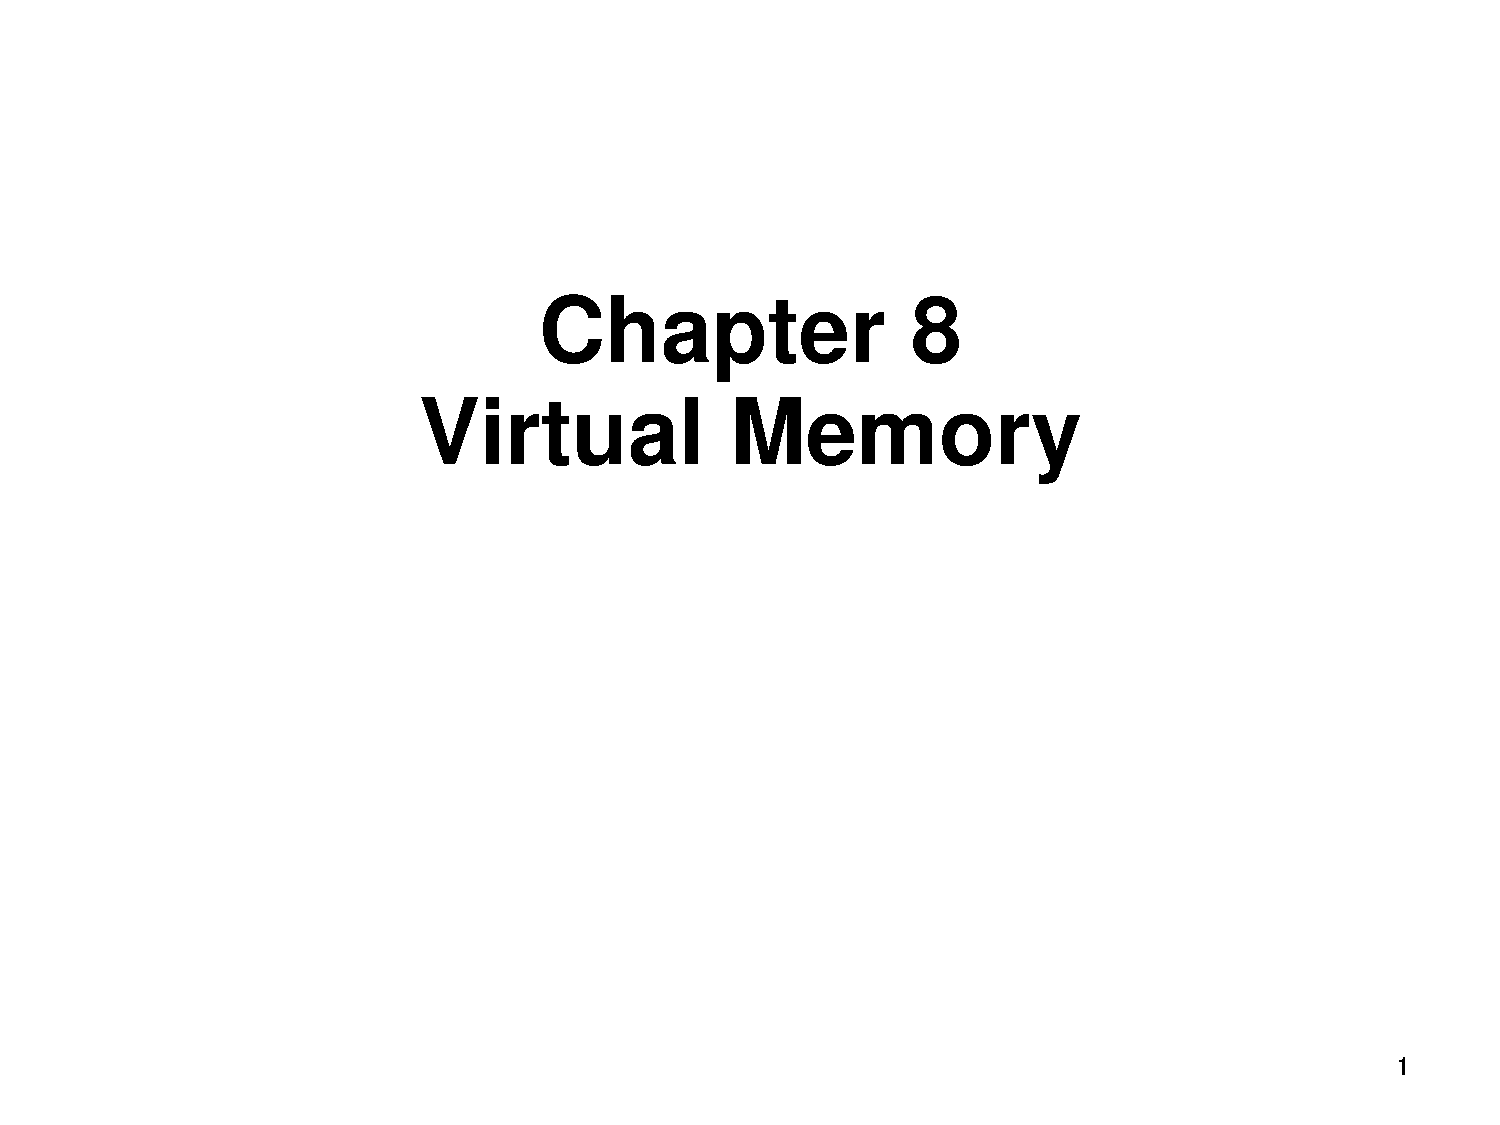
\includepdf[page=48]{08.pdf}
If we only bring in pages when we need them we will get a lot of faults. We want to load multiple pages at a time to take advantage of disk properties.
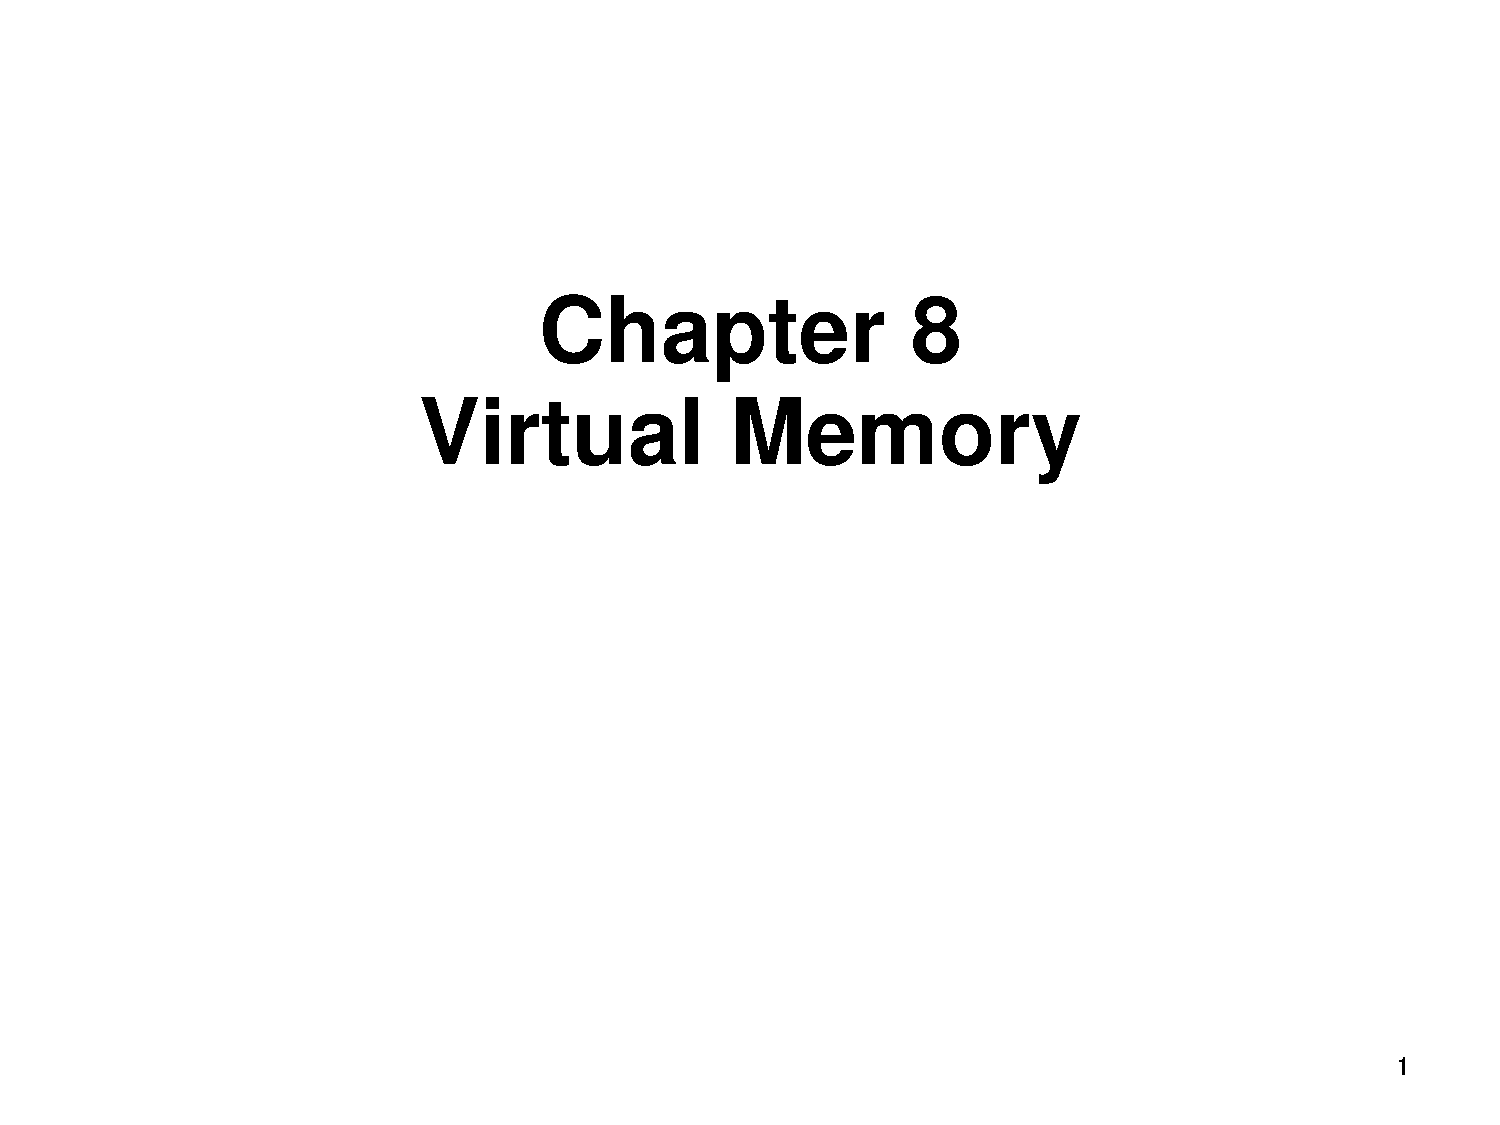
\includepdf[page=49]{08.pdf}
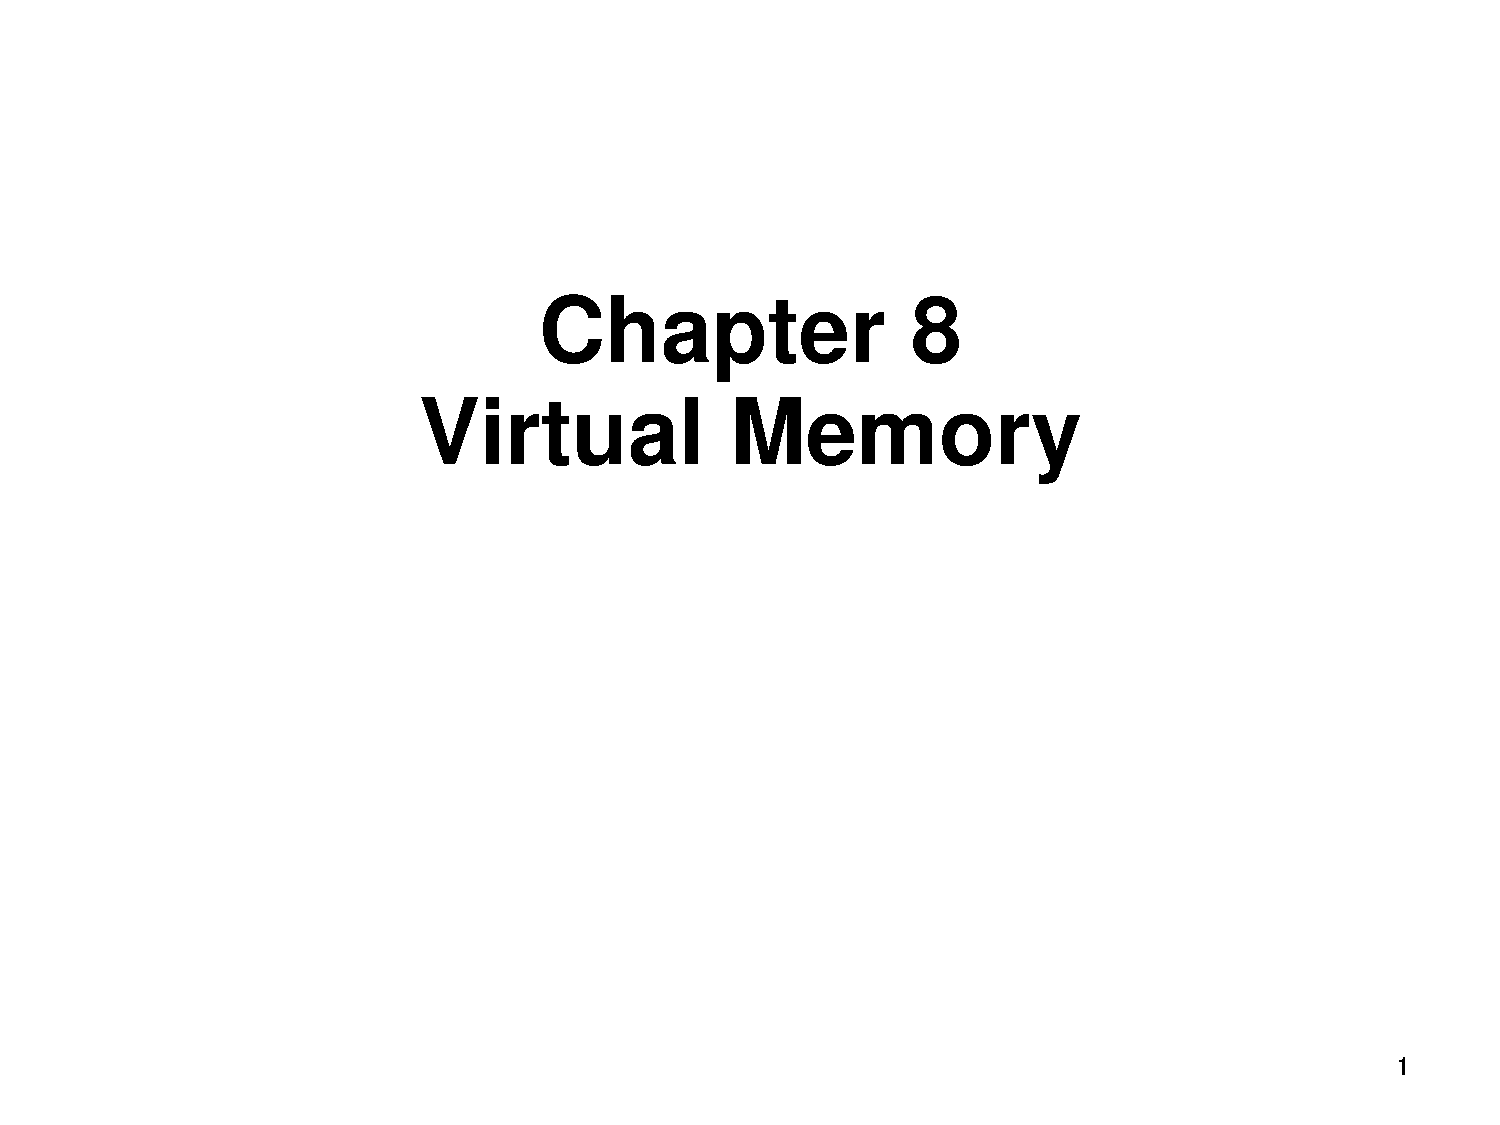
\includepdf[page=50]{08.pdf}
\includepdf[page=51]{08.pdf}
Here we want to use the principle of locality. If you recently used something nearby you will probably need it soon. We need to know how many pages need to be allocated and if we need to look at the global scope to replace other pages for the process. Now we have a set of pages to be replaces we chose a specific one to dump.
\includepdf[page=52]{08.pdf}
Frame locking is the ability to lock frames into memory (frames that we can never remove from memory).
\includepdf[page=53]{08.pdf}
Optimal policy is to look into the future and magically know what we need so that there are never any faults.
\includepdf[page=54]{08.pdf}
The next best is the policy of least recently used. The memory that has been unused for the longest period of time you probably won't need. This builds on the principle of locality. There is, however, a ton of overhead to keep up the time stamps and scan for the oldest. This overhead makes it actually pretty shitty.
\includepdf[page=55]{08.pdf}
This is considered the low hanging fruit that everyone uses. Here we just swap out the oldest memory using a circular buffer. This one is also pretty bad at guessing what is needed.
\includepdf[page=56]{08.pdf}
This is a good compromise between LRU and FIFO. We have a bit that approximates if it was used recently.
\includepdf[page=57]{08.pdf}
We maintain a circular buffer of memory. We keep a pointer to the last place that we loaded. From there we scan until we find a use bit that is 0 and for every page we have to jump over we set its use bit to 0.
\includepdf[page=58]{08.pdf}
\includepdf[page=59]{08.pdf}
OPT: since one is not used in the future we swap it for five. then we see that two is used farthest in the future so we swap it for four

LRU: we see that three was the least recently used so we swap it for five. same logic for why we swap one for four, so on and so forth

FIFO: and fifo is shit. really shit

CLOCK: here grey denotes used, blue denotes not. While its not as good as LRU it does beat FIFO
\includepdf[page=60]{08.pdf}
Maintain a free page list and modified page list. This lets us write out the modified pages in bulk since physical disks are better at stream than random write.
\includepdf[page=61]{08.pdf}
How many pages of a process do we keep in memory. We call this the resident set size. We want it to be small so we can have more processes but large so that we dont have as many faults. This is usually drawn as a function and look for the best result.
\includepdf[page=62]{08.pdf}
With fixed allocation we give each process a fixed number of pages and for faults we replace within the process. We maintain the replacement data structures (clock, fifo, etc) for each process.

With variable allocation the number of pages can vary over the life of the process.
\includepdf[page=63]{08.pdf}
\includepdf[page=64]{08.pdf}
\includepdf[page=65]{08.pdf}
\includepdf[page=66]{08.pdf}
\includepdf[page=67]{08.pdf}
Missed some stuff above this and got a smidge lost. Need to study from textbook
\includepdf[page=68]{08.pdf}
What the working set does it try to approximate the base line that is stable for use.
\includepdf[page=69]{08.pdf}
The working set is a subset of the resident set.

We use a sliding window operator to watch the working set of a process. We remove pages from the resident set but no the working set (dump stuff you havent used recently or often). Then we only allow a process to execute when its working set is in memory.

Some problems with this is that we are relying on the process's past to infer about its future which is seen from the above line graph where mode changes caused big spikes. It is also hard to implement because we need time-stamping to implement LRU for replacement which causes overhead.
\includepdf[page=70]{08.pdf}
This is how we deal with pages that ned to be replaces (if it was moddified we need to write it back to memory). We could do a deamnd cleaning which cleans every page that needs to go out. This is shitty because memory is bad at random access. The alternative of this is to batch pages together to increase how much we get done per write.
\includepdf[page=71]{08.pdf}
\includepdf[page=72]{08.pdf}
\includepdf[page=73]{08.pdf}
The mean time between page faults should be equal to the times process fault (time spent on writing pages) to get the optimal CPU utilization. Neat.
\includepdf[page=74]{08.pdf}
\includepdf[page=75]{08.pdf}



\end{document}
